%!TEX root = ../Calculo20.tex
%!TEX TS-program = pdflatex
%!TEX encoding = UTF-8 Unicode
\chapter{Cálculo diferencial}

\pagestyle{temas}
\thispagestyle{primera}

\paragraph{Contenidos}\ 

\vspace{-1em}
\begin{itemize}
\item
{\scshape Lección \thechapter.1: Curvas parametrizadas.}
Estudio de curvas parametrizadas.
Representación gráfica.
Asíntotas.
Curvas polares.
Cónicas.

\item
{\scshape Lección \thechapter.2: Campos escalares.}
Campos escalares lineales.
Derivadas direccionales, derivadas parciales y diferenciabilidad.
Vector gradiente.
Plano tangente a una superficie.
Derivadas de orden superior.

\item
{\scshape Lección \thechapter.3: Optimización de campos escalares.}
Extremos locales.
Clasificación de puntos críticos con la matriz hessiana.
Extremos condicionados y multiplicadores de Lagrange.
Extremos absolutos.
\end{itemize}

\paragraph{Prerrequisitos:}
Conocimientos básicos de álgebra lineal y geometría 
(ecuaciones de una recta, vectores, etc.). Trigonometría. Cálculo de límites y derivación. Representación gráfica de funciones de una variable (determinar dominio, puntos de corte con los ejes, intervalos de crecimiento y decrecimiento, extremos, intervalos de concavidad y convexidad, puntos de inflexión, etc.)


\paragraph{Objetivos:}
Los objetivos del tema son: reconocer una curva a partir de una parametrización y estudiar sus caracteristicas, incluidas las curvas polares;
reconocer y saber identificar las características de las curvas cónicas;
saber calcular y aplicar las propiedades del vector gradiente de un campo escalar;
plantear y resolver problemas de optimización de campos escalares.

\newpage
\paragraph{Resultados de aprendizaje}\ 

\vspace{-1em}
\begin{itemize}
\item
\textbf{Curvas parametrizadas y polares:}
Representar curvas parametrizadas y polares.
Hallar la recta tangente y la recta normal a una curva en un punto.
Saber determinar puntos de tangencia horizontal y puntos de tangencia vertical.
Saber determinar las asíntotas de una curva parametrizada.

\item
\textbf{Cónicas en su posición típica:}
Identificar y deducir las características de una cónica (degenerada o no) a partir de su expresión $P(x,y)=0$ (ejes, vértices, centro, asíntotas,\dots), siendo $P$ un polinomio de grado 2 sin término $xy$.
Obtener una parametrización de una cónica a partir de su ecuación normalizada.
Obtener la ecuación y parametrización de una cónica a partir de determinadas características.

\item
\textbf{Campos escalares:}
Hallar el vector gradiente.
Utilizar el vector gradiente para obtener propiedades geométricas (plano tangente, rectas normales, ortogonalidad de superficies o curvas,\dots).
Calcular derivadas direccionales.
Utilizar el vector gradiente como la dirección en donde la derivada direccional es máxima.

\item
\textbf{Optimización:}
Hallar y clasificar puntos críticos de campos de dos variables usando la matriz hessiana o el comportamiento del campo en rectas o curvas que pasan por el punto crítico.
Hallar y clasificar puntos críticos de campos de dos variables con una restricción, usando multiplicadores de Lagrange o reducción de variables.
Hallar los máximos y mínimos absolutos de campos de dos variables sobre regiones acotadas.
\end{itemize}

\newpage
\section{Curvas planas}\label{lec:curvas}%parametrizadas}

El objetivo último de las matemáticas es \emph{modelizar} el mundo real. Es decir, representar y describir diversos aspectos del mundo real mediante conceptos matemáticos que ayuden a estudiarlo.
En particular, en esta lección nos centramos en la representación de objetos y figuras que genéricamente denominamos \emph{lugares geométricos}.
Podemos entender fácilmente cuál es nuestro objetivo con el siguiente problema:
\emph{traza en un papel tres rectas que se corten formando un triángulo y luego dale indicaciones a un compañero para que haga exactamente el mismo dibujo}.
Seguramente, las indicaciones dadas estarán basadas en objetos matemáticos: sistemas de referencias, distancias, ángulos,\dots

Para lograr resolver el problema anterior no se necesitan demasiados elementos, pero ¿cómo haríamos lo mismo si en lugar de rectas quisiéramos describir
una \emph{curva}? Este es el problema general que abordamos en esta lección.
Aprenderemos a describir curvas, a dibujarlas a partir de una descripción y, en particular, conoceremos un conjunto de curvas ampliamente usadas en matemáticas y física y que se denominan \emph{cónicas}.

Aunque toda la teoría que vamos a mostrar se puede aplicar fácilmente a curvas en el espacio o incluso en dimensiones mayores a 3, nos vamos a centrar solamente en curvas en el plano.

\begin{rawhtml}
<p style="text-align: center;"><iframe width="560" height="316" src="https://www.youtube.com/embed/rNDafG6brzs?list=PL2rtpLKW91qaoiK4EarXJ63UTuWldV2ul" frameborder="0" allowfullscreen=""></iframe></p>
\end{rawhtml}

\subsection{Curvas parametrizadas}

Es fácil imaginar una curva como una recta a la que se aplica un determinada deformación. Es decir, una curva es una figura de una única dimensión pero que no sigue una dirección constante.
Esta imagen intuitiva nos lleva a la representación más sencilla de una curva: la descripción de cada punto de la misma en función de \emph{un parámetro}.
Por ejemplo, si queremos describir la trayectoria que seguimos en un paseo, bastaría con dar nuestra posición en cada instante de tiempo; en este caso, el tiempo sería el parámetro que describe la curva trazada por nuestra trayectoria.

\begin{definicion} Un conjunto $C\subset\mathbb{R}^2$ se dice que es una \emph{curva parametrizada} si existe un intervalo $I\subseteq \mathbb{R}$ y dos funciones $x\colon I\to \mathbb{R}$, $y\colon I\to \mathbb{R}$ tales que
\[
C=\{(x(t),y(t)) \mid t\in I\}
\]
\end{definicion}

Habitualmente, presentamos las curvas parametrizadas escribiendo:
\[
\begin{cases}
& X = x(t)\\
& Y = y(t)\\
& t\in I
\end{cases}
\]
o de forma más compacta $(X,Y)=(x(t),y(t))$, $t\in I$. Estas ecuaciones se denominan \emph{ecuaciones paramétricas de la curva} y la variable $t$ se
denomina \emph{parámetro}.

\begin{ejemplo}
\emph{Ecuaciones paramétricas de una recta.}
La recta que pasa por un punto $(a,b)$ en la dirección del vector $\boldsymbol{v}=(v_1,v_2)$ es:
\[
\begin{cases}
& X = a + v_1 t\\
& Y = b + v_2 t\\
& t\in\mathbb{R}
\end{cases}
\]
En este caso, el parámetro $t$ representa la distancia al punto $(a,b)$, siendo la unidad de medida el módulo del vector $\boldsymbol{v}$, es decir, $\|\boldsymbol{v}\|=\sqrt{v_1^2+v_2^2}$.

En la figura siguiente, representamos la recta que pasa por $(-3,3)$ y toma la dirección $(2,1)$, es decir, $(X,Y)=(-3,3)+t(2,1) = (-3+2t,3+t)$. En la figura, destacamos el punto correspondiente a $t=5$.

\ \hfill
\begin{tikzpicture}[x=1em,y=1em]
\pgfsetlinewidth{.5pt}
\draw[-stealth] (-8.8,0) -- (10.2,0) node[right] {$X$}; 
\draw[-stealth] (0,3.5) -- (0,9.7) node[above] {$Y$};
\draw (0,-.4) -- (0,2.3);
\draw[thick] (-8.6,.2) -- (10,9.5);
\draw (-2.9,3.3) node[left]{$(-3,3)$};
\draw[thick,*-latex] (-3,3) -- (-1,4);
\draw[thick,-latex] (-1,4) -- (1,5);
\draw[thick,-latex] (1,5) -- (3,6);
\draw[thick,-latex] (3,6) -- (5,7);
\draw[thick,-latex] (5,7) -- (7,8);
\draw[<-,out=290,in=180] (7.05,7.95) to (6,4) node[right] {$(X,Y)=(-3,3)+5(2,1)$};
\draw (0,3.8) node[below] {$\boldsymbol{v}=(2,1)$};
\end{tikzpicture}
\hfill
\fej
\end{ejemplo}

En este ejemplo hemos utilizado la notación $\|\boldsymbol{v}\|$ para representar el módulo del vector $\|\boldsymbol{v}\|$; esta función se denomina igualmente \emph{norma} y otras notaciones que podemos encontrar en la bibliografía son $|\boldsymbol{v}|$ ó $\|\boldsymbol{v}\|_2$.

\begin{rawhtml}
<p style="text-align: center;"><iframe width="560" height="316" src="https://www.youtube.com/embed/Gl1NpOMpHxM?list=PL2rtpLKW91qaoiK4EarXJ63UTuWldV2ul" frameborder="0" allowfullscreen=""></iframe></p>
\end{rawhtml}

El uso de letras en matemáticas es imprescindible para representar variables, constantes, parámetros,\dots Ya hemos advertido que habitualmente usamos letras cursivas (mayúsculas o minúsculas) para representar variables que a su vez pueden corresponder a cualquier objeto matemático: números naturales, racionales, reales, complejos, puntos en un plano, vectores,\dots
También hemos podido observar que solemos usar determinadas letras para objetos específicos: $x$ para incógnitas de ecuaciones o para la abscisa de puntos; $n$, $k$ para números naturales; $z$ para números complejos; $t$ para representar el tiempo,\dots
Debe de quedar claro que estas identificaciones se hacen por tradición y para ayudar a la lectura de fórmulas y expresiones, pero no es obligatorio y en muchos casos no respetaremos estas asociaciones.

Por otra parte, en el ejemplo anterior, hemos usado letras en negrita para representar vectores. Siguiendo con la idea del párrafo anterior, es habitual usar algún elemento distintivo para estos objetos, como la letra negrita que usaremos en el curso o flechas sobre las letras que podemos encontrar en algunos textos.
También debe quedar claro que estos elementos no son imprescindibles y solo se usan para facilitar la lectura.
%
\begin{ejemplo}
\emph{Parametrización de un segmento.}
En el ejemplo anterior, las ecuaciones se corresponden con una recta infinita.
Sin embargo, es frecuente que solo estemos interesados en el segmento que une dos puntos $P_1$, $P_2$.
\begin{center}
\begin{tikzpicture}[x=4em,y=4em]
\pgfsetlinewidth{.5pt}
\draw[-stealth] (-1.8,0) -- (2.3,0) node[right] {$X$}; 
\draw[-stealth] (0,-.4) -- (0,1.8) node[above] {$Y$};
\draw[thick,-latex] (-1.6,1.2) node[left]{$P_1$} -- (2,.6) node[right]{$P_2$};
\draw[<-,out=75,in=180] (0.92,.78) to (1.5,1.2) node[right] {$(X,Y)=(1-t)P_1+tP_2$};
\end{tikzpicture}
\end{center}

Para parametrizar este segmento, tomamos el vector director $\boldsymbol{v}=\overrightarrow{P_1P_2}=P_2-P_1$ y aplicamos las ecuaciones del ejemplo anterior: $(X,Y)=P_1+t\overrightarrow{P_1P_2}$.
Sustituyendo el vector por su definición obtenemos
\begin{equation}\label{par:seg}
(X,Y)= (1-t)P_1 + tP_2,\quad t\in [0,1]
\end{equation}
En este caso, el parámetro $t$ es la proporción de la distancia a $P_1$ respecto de la longitud del segmento, es decir, si $Q=(x(t),y(t))$ es el punto correspondiente al valor $t$ del parámetro, entonces $t=\frac{|P_1Q|}{|P_1P_2|}$.
Por ejemplo, el segmento que une los puntos $(-1,-1)$ con $(0,2)$ es:
\[
(X,Y) = (1-t)(-1,-1)+t(0,2)=(t-1,3t-1),\quad t\in[0,1]
\]
Es interesante observar que esta parametrización no da únicamente información de los puntos que forman el segmento, también describe cómo lo recorremos.
En concreto, en la ecuación~\eqref{par:seg}, el valor~$t=0$ nos devuelve el punto $P_1$, mientras que el valor $t=1$ nos devuelve $P_2$, es decir, recorremos el segmento desde el punto~$P_1$ al~$P_2$.
La siguiente parametrización también corresponde al mismo segmento, pero recorriéndolo en sentido contrario:
%
\begin{equation}
(X,Y)= (1-t)P_2 + tP_1 ,\quad t\in [0,1]\tag*{\fej}
\end{equation}
%
\end{ejemplo}
\begin{rawhtml}
<p></p>
\end{rawhtml}
\begin{ejemplo}
Ya sabemos que todas las funciones reales de variable real pueden representarse mediante su gráfica. Esta gráfica es un ejemplo de curva parametrizada que se denomina \emph{grafo}:
\[
\mathrm{gr}(f)=\{(t,f(t))\mid t\in \operatorname{Dom}(f)\}
\]
Es decir, las siguientes ecuaciones parametrizan el grafo:
\[
\begin{cases}
& X = t\\
& Y = f(t)\\
& t\in \operatorname{Dom}(f)
\end{cases}
\]
En este caso, el parámetro coincide con la abscisa del punto.
Se podría pensar que todas las curvas pueden ser representadas como grafos de una función, sin embargo, esto no es cierto.
Por ejemplo, ninguna función tiene como gráfica a toda una circunferencia, aunque sí trozos de la misma.\fej
\end{ejemplo}

El problema de dar la parametrización de una curva descrita mediante propiedades geométricas suele ser bastante sencillo, ya que, en la mayoría de los casos, solo necesitamos aplicar elementos básicos de geometría.
%
\begin{ejemplo}
En este ejemplo, parametrizamos la curva que se denomina \emph{cicloide} y que se define como sigue: \emph{curva que describe un punto fijo de una circunferencia que rueda sobre una recta}.
\begin{center}
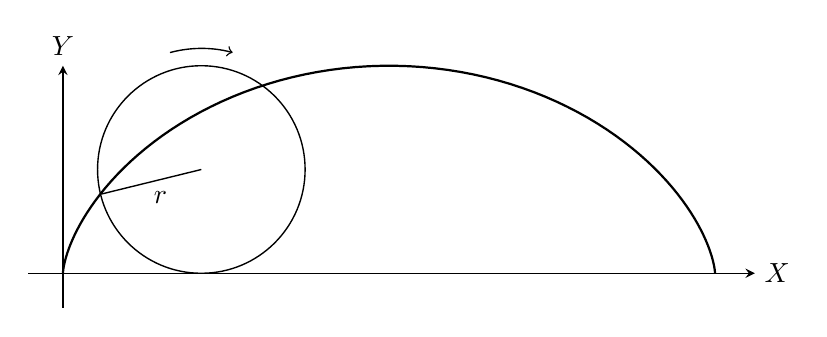
\begin{tikzpicture}[x=1.25em,y=1.25em]
\pgfsetlinewidth{.5pt}
\draw[-stealth] (-1,0) -- (20,0) node[right] {$X$}; 
\draw[-stealth] (0,-1) -- (0,6) node[above] {$Y$};
\draw[thick,domain=0:2*pi]
plot[samples=100] ({3*\x-3*sin(\x r)},{3-3*cos(\x r)});
\draw (4,3) circle (3);
\draw (4,3) -- (1.11,2.29);
\draw (3.3,2.2) node[left]{$r$};
\draw[<-] (4,3) +(75:3.5) arc (75:105:3.5);
\end{tikzpicture}
\end{center}
\begin{rawhtml}
** Añadir gif cicloide **
\end{rawhtml}

Si elegimos como parámetro el ángulo de giro de la circunferencia, podemos deducir las ecuaciones de la cicloide:
\begin{center}
\begin{tabular}{c@{\qquad\qquad}c}
%
$\left\{\begin{array}{cl}
& x(\theta)=r(\theta-\operatorname{sen} \theta)\\
& y(\theta)=r(1-\cos \theta) \\
\end{array}\right.$ &
%
\raisebox{-4em}{
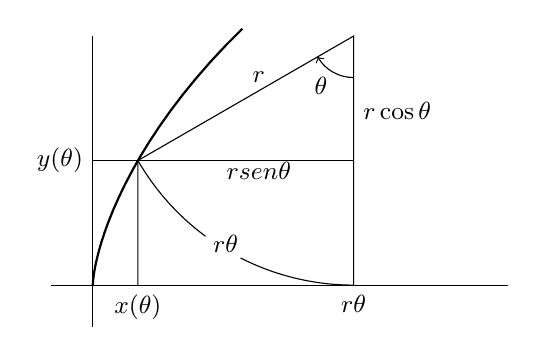
\begin{tikzpicture}[x=3em,y=3em]
%\pgfsetlinewidth{.5pt}
\draw (-.5,0) -- (5,0); 
\draw (0,-.5) -- (0,3);
\draw[thick,domain=0:1.6]
plot ({3*\x-3*sin(\x r)},{3-3*cos(\x r)});
\draw (3.142,3) +(210:3) arc (210:233.5:3);
\draw (3.142,3) +(243:3) arc (243:270:3);
\draw[->] (3.142,3) +(270:.5) arc (270:210:.5);
\draw (.543,0) -- (.543,1.5) -- (3.142,3) -- (3.142,0);
\draw (0,1.5) -- (3.142,1.5);
\draw (3.142,2.1) node[right]{\small $r\cos \theta$};
\draw (2,1.6) node[below]{\small $r\operatorname{sen} \theta$};
\draw (0,1.5) node[left]{\small $y(\theta)$};
\draw (.543,0) node[below]{\small $x(\theta)$};
\draw (3.142,0) node[below]{\small $r\theta$};
\draw (2,2.5) node {\small $r$};
\draw (2.75,2.4) node {\small $\theta$};
\draw (1.6,.5) node {\small $r\theta$};
\end{tikzpicture}}
\end{tabular}
\end{center}
\fej
\end{ejemplo}

El concepto matemático que nos ayuda a manejar formalmente las ecuaciones paramétricas es el de \emph{función vectorial de variable real}.
%
\begin{definicion}
Una \emph{función vectorial de variable real} con dominio $\mathit{D}\subset \mathbb{R}$ es una
aplicación $\boldsymbol{f} \colon \mathit{D}\to \mathbb{R}^n$. Esta función $\boldsymbol{f}$ viene determinada por $n$ funciones reales de variable real, $f_i\colon
\mathit{D}\subset\mathbb{R} \to\mathbb{R}$, de modo que $\boldsymbol{f}(t)=(f_1(t),\dots ,f_n(t))$.
%; escribiremos$\boldsymbol{f}=(f_1,\dots ,f_n)$
\end{definicion}

Habitualmente, trabajaremos con curvas con un aspecto suave y sin rupturas; para conseguir esto, necesitaremos que las parametrizaciones tengan ciertas características.

\begin{definicion} Sea $\boldsymbol{f}=(f_1,\dots ,f_n) \colon \mathit{D}\subset \mathbb{R}\to
\mathbb{R}^n$:
\begin{enumerate}
\item Decimos que $\boldsymbol{f}$ es continua en $a\in \mathit{D}$ si todas la funciones $f_i$ son continuas en $a$. Decimos que $\boldsymbol{f}$ es continua en $\mathit{D}$ si lo es en cada punto.
%; es decir, si $\lm[t]{a}\boldsymbol{f}(t)=\boldsymbol{f}(a)$.
\item Decimos que $\boldsymbol{f}$ es derivable o diferenciable en $a\in \mathit{D}$, si todas la funciones $f_i$ son derivables en $a$ y el vector $\boldsymbol{f}'(a)=(f'_1(a),\dots,f'_n(a))$ se denomina derivada de~$\boldsymbol{f}$ en~$a$.
\end{enumerate}
\end{definicion}

Si una curva $(x(t),y(t))$ es continua, se puede dibujar ``un solo trazo'' o ``sin levantar el lápiz del papel''.
Sabemos que la gráfica de una función derivable tiene un aspecto ``suave'', ``sin picos'', sin embargo, para que una curva parametrizada tenga este aspecto, no es suficiente con que la parametrización sea diferenciable, necesitaremos que sea \emph{regular}.

\begin{definicion}
Una curva $(x(t),y(t))$, $t\in I$, es \emph{regular en $t_0$} si es diferenciable en $t_0$ y $(x'(t_0),y'(t_0))\ne(0,0)$. 
\end{definicion}

\subsubsection{Representación de curvas}

En general, no es fácil identificar una curva a partir de una parametrización,
sin embargo, no resulta difícil deducir determinadas características que ayudan a esbozar su forma.
A continuación mostramos algunas:
\begin{itemize}
\item
Si $x(t)$ es creciente en un intervalo, la curva se recorre de izquierda a derecha; si es decreciente, se recorre de derecha a izquierda.
\item
Si $y(t)$ es creciente en un intervalo, la curva se recorre de abajo hacia arriba; si es decreciente, se recorre de arriba hacia abajo.
\item
La ecuación $x(t)=0$ determina los puntos de corte con el eje $OY$ y la ecuación $y(t)=0$ determina los puntos de corte con el eje $OX$.
\end{itemize}
%
\begin{ejemplo}\label{ej:parapar}
Vamos a esbozar la curva con la siguiente parametrización:
\[
\begin{cases}
& x(t)=t^2-2t+1\\
& y(t)=2-2t^2\\
& t\in\mathbb{R}
\end{cases}
\]
%
En primer lugar, vamos a representar gráficamente las funciones $x(t)$ e $y(t)$; para ello, son suficientes los conocimientos de cálculo en una variable y por ello no mostramos los detalles
\begin{center}
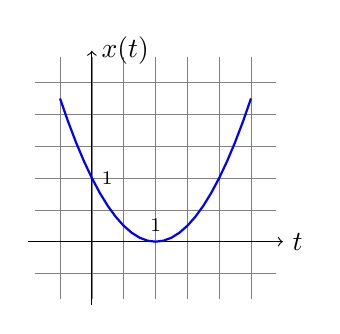
\begin{tikzpicture}[x=2.3em,y=2.3em]
\draw[very thin,color=gray,step=.5] (-.9,-.9) grid (2.9,2.9); 
\draw[->] (-1,0) -- (3,0) node[right] {$t$}; 
\draw[->] (0,-1) -- (0,3) node[right] {$x(t)$};
\draw[color=blue,thick,domain=-.5:2.5]
plot (\x,\x*\x-2*\x+1);
\draw (0,1) node[right] {$\scriptstyle 1$};
\draw (1,0) node[above] {$\scriptstyle 1$};
\end{tikzpicture}\qquad\quad
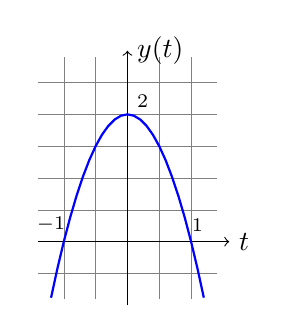
\begin{tikzpicture}[x=2.3em,y=2.3em]
\draw[very thin,color=gray,step=.5] (-1.4,-.9) grid (1.4,2.9); 
\draw[->] (-1.4,0) -- (1.6,0) node[right] {$t$}; 
\draw[->] (0,-1) -- (0,3) node[right] {$y(t)$};
\draw[color=blue,thick,domain=-1.2:1.2]
plot (\x,2-2*\x*\x);
\draw (-1.2,0) node[above] {$\scriptstyle -1$};
\draw (0,2.2) node[right] {$\scriptstyle 2$};
\draw (1.1,0) node[above] {$\scriptstyle 1$};
\end{tikzpicture}
\end{center}
La función $x$ pasa de decrecer a crecer en $t=1$ y la función $y$ pasa de crecer a decrecer en $t=0$; los puntos correspondientes a estos valores del parámetro son:
%
\[
(x(0),y(0))=(1,2),\qquad
(x(1),y(1))=(0,0)
\]
Por lo tanto:
hasta $(1,2)$ la curva se recorre de derecha a izquierda y de abajo a arriba; desde $(1,2)$ hasta $(0,0)$ la curva se recorre de derecha a izquierda y de arriba a abajo; desde el punto $(0,0)$ se recorre de izquierda a derecha y de arriba a abajo.
Con la información anterior y situando los puntos de corte con los ejes, es fácil dibujar la curva:
\begin{center}
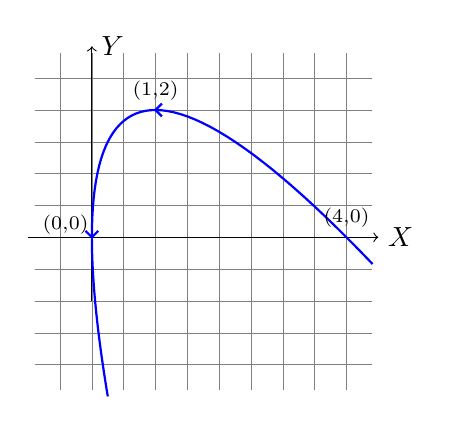
\begin{tikzpicture}[x=2.3em,y=2.3em]
\draw[very thin,color=gray,step=.5] (4.1,-2.4) grid (9.4,2.9); 
\draw[->] (4,0) -- (9.5,0) node[right] {$X$}; 
\draw[->] (5,-1) -- (5,3) node[right] {$Y$};
\draw[color=blue,thick,domain=-1.1:0]
plot (\x*\x-2*\x+6,2-2*\x*\x);
\draw (9,0) node[above] {$\scriptstyle (4,0)$};
\draw (6,2) node[above] {$\scriptstyle (1,2)$};
\draw[color=blue,thick] (6.1,1.9)--(6,2)--(6.1,2.1);
%
\draw[color=blue,thick,domain=0:1]
plot (\x*\x-2*\x+6,2-2*\x*\x);
\draw (5.1,.2) node[left] {$\scriptstyle (0,0)$};
\draw[color=blue,thick] (4.9,.1)--(5,0)--(5.1,.1);
\draw[color=blue,thick,domain=1:1.5]
plot (\x*\x-2*\x+6,2-2*\x*\x);
\end{tikzpicture}\\[-1em]
\fej
\end{center}
\begin{rawhtml}
<p style="text-align: center;"><iframe width="560" height="316" src="https://www.youtube.com/embed/1IHvOFgUKeI?list=PL2rtpLKW91qaoiK4EarXJ63UTuWldV2ul" frameborder="0" allowfullscreen=""></iframe></p>
\end{rawhtml}
\end{ejemplo}

Como hemos mencionado antes, si una curva es regular en un punto, entonces en ese punto la curva no tiene un pico. Geométricamente, esto se traduce en que es posible trazar una recta tangente a la curva en ese punto.
Esta recta tangente se define a partir de la derivada de la parametrización.
%
\begin{definicion} Sea $X=x(t)$, $Y=y(t)$, $t\in I$ una parametrización de la curva~$C$.
Si $(x'(t_0),y'(t_0))\ne(0,0)$, las siguientes ecuaciones determinan la \emph{recta tangente} a
$C$ en el punto $(x(t_0),y(t_0))$:
\begin{align*}
x & = x(t_0)+\lambda x'(t_0) \\
y & = y(t_0)+\lambda y'(t_0)
\end{align*}
En donde $\lambda$ es el parámetro de la recta.
\end{definicion}
%
En la definición anterior, la recta tangente se define usando una parametrización; podemos eliminar el parámetro para obtener su ecuación cartesiana:
\[
x'(t_0)(y-y(t_0))=y'(t_0)(x-x(t_0))
\]
%
\begin{ejemplo}
Si la curva es el grafo de una función real de variable real, es decir, $(X,Y)=(t,f(t))$, entonces, $x(t_0)=x_0$, $y(t_0)=f(x_0)$, $x'(t_0)=1$ e $y'(t_0)=f'(t_0)$. Sustituyendo en la ecuación anterior, obtenemos la conocida expresión de la recta tangente a la gráfica de una función.
\begin{equation}
y-f(x_0)=f'(x_0)(x-x_0)\tag*{\fej}
\end{equation}
%Por ejemplo, para la función $f(x)=\operatorname{sen} x$, la recta tangente en el punto $(\frac{\pi}4,\sqrt2/2)$ de su gráfica es
%\begin{equation}
%Y-\frac{\sqrt2}2 = \frac{\sqrt2}2\left(X-\frac{\pi}4\right)\tag*{\fej}
%\end{equation}
\end{ejemplo}
\begin{rawhtml}
<p></p>
\end{rawhtml}
\begin{ejemplo}
En la curva del ejemplo~\ref{ej:parapar},
\[
\begin{cases}
& x(t)=t^2-2t+1\\
& y(t)=2-2t^2\\
& t\in\mathbb{R}
\end{cases}
\]
el vector tangente en $(x(t),y(t))$ es:
\[
(x'(t),y'(t))=(2t-2,-4t)
\]
Por lo tanto, el vector tangente en $t=0$ es $(x'(0),y'(0))=(-2,0)$ y la recta tangente en $(x(0),y(0))=(1,2)$ es paralela al eje $OX$;
el vector tangente en $t=1$ es $(0,-4)$ y la recta tangente en $(x(1),y(1))=(0,0)$ es paralela al eje $OY$.\fej
\end{ejemplo}
%
Otra interpretación del vector derivada proviene del campo de la física.
Si la parametrización corresponde a la trayectoria de un movimiento en función del tiempo, la derivada se corresponde con el vector velocidad.

\begin{rawhtml}
<p style="text-align: center;"><iframe width="560" height="316" src="https://www.youtube.com/embed/Fj_xcQZSZOA?list=PL2rtpLKW91qaoiK4EarXJ63UTuWldV2ul" frameborder="0" allowfullscreen=""></iframe></p>
\end{rawhtml}

\subsubsection{Asíntotas}\label{sec:asintotas}
Intuitivamente, una recta es asíntota de una curva si la distancia entre ambas va decreciendo a~0.
% al desplazarnos sobre la curva.
%En el ejercicio~\ref{ex:as2}, se recuerda como determinar las asíntotas del grafo de una función; a continuación las estudiamos sobre una curva general.
El estudio de la existencia de una asíntota es diferente dependiendo de si la recta es vertical, horizontal u oblicua.
El siguiente resultado muestra las condiciones que debemos comprobar para determinar la existencia de asíntotas.

\begin{proposicion}
Consideremos una curva $(x(t),y(t))$, $t\in I$.
\begin{enumerate}
\item
Si para un valor del parametro $t_0$, $\displaystyle\lim_{t\to t_0}x(t)=a$ y $\displaystyle\lim_{t\to t_0}y(t)=\infty$, entonces la recta $x=a$ es una asíntota vertical de la curva.
\item
Si para un valor del parametro $t_0$, $\displaystyle\lim_{t\to t_0}x(t)=\infty$ y $\displaystyle\lim_{t\to t_0}y(t)=a$, entonces la recta $y=a$ es una asíntota horizontal de la curva.
\item
Si para un valor del parametro $t_0$,
\[
\begin{array}{l@{\qquad}l}
\displaystyle\lim_{t\to t_0}x(t)=\pm\infty, &
\displaystyle\lim_{t\to t_0}y(t)=\pm\infty, \\
\displaystyle\lim_{t\to t_0}\dfrac{y(t)}{x(t)}=m\in\mathbb{R}, &
\displaystyle\lim_{t\to t_0}(y(t)-mx(t))=n\in\mathbb{R}
\end{array}
\]
entonces $y=mx+n$ es una asíntota de la curva.
%, en donde $n=\lim_{t\to t_0}(y(t)-mx(t))$.
\end{enumerate}
Los tres apartados se verifican igualmente si consideremos $t_0$ igual a $\pm\infty$.
\end{proposicion}
%
Obsérvese que las asíntotas se localizan en valores del parámetro que no pertenecen al dominio de, al menos, una de las dos coordenadas.

\begin{figure}
\begin{center}
\begin{tikzpicture}[x=1.5em,y=1.5em]
\draw[-stealth] (-5,0) -- (8,0) node[right] {$X$}; 
\draw[-stealth] (0,-5) -- (0,5) node[right] {$Y$};
\draw[thin,dashed] (-4.7,-4.7) -- (5,5);
\draw[thick,domain=-5:5,samples=50,variable=\x]
plot ({(7-\x*\x*\x)/(1+\x*\x)},{(-\x*\x*\x)/(1+\x*\x)});
\end{tikzpicture}
\end{center}
\caption{Curva del ejemplo~\ref{ej:asint}.}\label{fig:ej-asint}
\end{figure}

\begin{ejemplo}\label{ej:asint}
Vamos a estudiar si la siguiente curva tiene asíntotas.
\[
x(t)=\frac{7-t^3}{1+t^2},\qquad
y(t)=\frac{-t^3}{1+t^2},\qquad t\in\mathbb{R}
\]
El dominio de las funciones $x(t)$ e $y(t)$ es $\mathbb{R}$, y por lo tanto, si la curva tiene asíntotas, estas deben estar en $+\infty$ o en $-\infty$.
Las dos funciones verifican la tercera condición en los dos casos:
\begin{alignat*}{2}
\lim_{t\to +\infty}x(t)=\lim_{t\to +\infty}\frac{7-t^3}{1+t^2}&=-\infty, &\qquad\qquad
\lim_{t\to +\infty}y(t)=\lim_{t\to +\infty}\frac{-t^3}{1+t^2}&=-\infty \\
\lim_{t\to -\infty}x(t)=\lim_{t\to -\infty}\frac{7-t^3}{1+t^2}&=\infty, & \qquad
\lim_{t\to +\infty}y(t)=\lim_{t\to -\infty}\frac{-t^3}{1+t^2}&=\infty
\end{alignat*}
Intentamos calcular las pendientes de las asíntotas:
\begin{align*}
\lim_{t\to +\infty}\frac{y(t)}{x(t)} & =
\lim_{t\to +\infty}\frac{-t^3}{1+t^2}\cdot\frac{1+t^2}{7-t^3}=
\lim_{t\to +\infty}\frac{-t^3}{7-t^3}= 1 \\
\lim_{t\to -\infty}\frac{y(t)}{x(t)} & =
\lim_{t\to -\infty}\frac{-t^3}{1+t^2}\cdot\frac{1+t^2}{7-t^3}=
\lim_{t\to -\infty}\frac{-t^3}{7-t^3}= 1
\end{align*}
Por lo tanto, si la curva tiene asíntotas, sus pendientes son igual a 1.
Terminamos de calcular los últimos límites que demuestran que efectivamente la curva tiene asíntotas.
\begin{align*}
\lim_{t\to +\infty}(y(t)-x(t))&=
\lim_{t\to +\infty}\left(\frac{-t^3}{1+t^2}-\frac{7-t^3}{1+t^2}\right)=
\lim_{t\to +\infty}\frac{-7}{1+t^2}=0\\
\lim_{t\to -\infty}(y(t)-x(t))&=
\lim_{t\to -\infty}\left(\frac{-t^3}{1+t^2}-\frac{7-t^3}{1+t^2}\right)=
\lim_{t\to -\infty}\frac{-7}{1+t^2}=0
\end{align*}
Por lo tanto, la recta $y=x$ es asíntota de la curva tanto en $+\infty$ como en $-\infty$ (ver figura~\ref{fig:ej-asint}).\fej
\end{ejemplo}

\subsection{Curvas polares}

Hemos visto en el tema anterior que una forma alternativa de representar los puntos de un plano es mediante \emph{coordenadas polares}.
En general, un sistema de coordenadas polares queda determinado por un punto $O$, llamado \emph{polo}, y una semirrecta con extremo en $O$, llamada \emph{eje polar}.
Dado un punto $Q$ en el plano, consideramos la semirrecta $R$ con extremo en el polo y que pasa por $Q$ (\emph{recta radial} del punto);
la posición de $Q$ en coordenadas polares se fija por \emph{distancia del punto al polo}, $r$, y el
\emph{ángulo $\theta$ entre el eje polar y la recta radial} medido en el sentido contrario a las agujas del reloj; el par
$(r,\theta)_P$ es la descripción por \emph{coordenadas polares} del punto~$Q$.

\begin{figure}
\begin{center}
\begin{tikzpicture}[x=2.5em,y=2.5em]
\draw[-stealth] (-2,0) -- (4,0) node[right] {$X$}; 
\draw[-stealth] (0,-1) -- (0,3) node[right] {$Y$};
\draw[dashed] (3,0)node[below]{$x$} -- (3,2) -- (0,2)node[left]{$y$};
\draw (0,0) -- (3,2) node[right]{$(x,y)=(r,\theta)_P$};
\draw[->] (0,0) +(0:1.5) arc (0:33:1.5); %+(210:3) 
\draw (1.7,.5)node{$\theta$};
\end{tikzpicture}
%\includegraphics{polares.pdf}
\end{center}
\caption{Sistema de representación polar.}%
\label{fig:sist-polar}
\end{figure}
%
El sistema cartesiano y el sistema polar se superponen identificando el polo con el origen de coordenadas y el eje polar con el semieje positivo de~$OX$, tal y como se muestra en la figura~\ref{fig:sist-polar}.
%
\begin{definicion}
Dada una función $f\colon \mathit{D}\subset\mathbb{R}\to\mathbb{R}$, llamamos \emph{curva polar} asociada a $f$ al conjunto de puntos $(f(\theta),\theta)_P$ del plano polar.
\end{definicion}
%
Es decir, la curva polar asociada a $f$ queda determinada por las siguientes ecuaciones paramétricas:
%
\[
\begin{cases}
& x=f(\theta)\cos\theta \\
& y=f(\theta)\operatorname{sen}\theta \\
& \theta\in \mathit{D}
\end{cases}
\]
Aunque la parametrización anterior permite estudiar las curvas polares como cualquier curva paramétrica, es conveniente utilizar las propiedades específicas de este tipo de curvas.

\begin{rawhtml}
<p style="text-align: center;"><iframe width="560" height="316" src="https://www.youtube.com/embed/BK7rav8q1gk?list=PL2rtpLKW91qaoiK4EarXJ63UTuWldV2ul" frameborder="0" allowfullscreen=""></iframe></p>
\end{rawhtml}

\begin{proposicion}
Si $f$ es derivable, $f(\theta_0)\ne 0$ y $f'(\theta_0)=0$, entonces la curva polar correspondiente y la circunferencia de centro en el origen y radio $|f(\theta_0)|$ son tangentes en el punto $(f(\theta_0),\theta_0)_P$.
\end{proposicion}
\begin{rawhtml}
<p></p>
\end{rawhtml}
\begin{proposicion}
Si $f$ es derivable y $f(\theta_0)=0$,
% y $f'(\theta_0)\ne 0$
entonces la recta radial con ángulo~$\theta_0$ es
tangente a la curva polar correspondiente en el origen de coordenadas.
\end{proposicion}

La demostración de este resultado es inmediata considerando la parametrización correspondiente a la curva polar:
\begin{align*}
x'(\theta)&=f'(\theta)\cos\theta-f(\theta)\operatorname{sen}\theta\\
y'(\theta)&=f'(\theta)\operatorname{sen}\theta+f(\theta)\cos\theta
\end{align*}
Si $f(\theta_0)=0$, el segundo sumando de las dos derivadas anteriores se anula al evaluarlas en $\theta_0$:
\begin{align*}
x'(\theta_0)&=f'(\theta_0)\cos\theta_0 \\
y'(\theta_0)&=f'(\theta_0)\operatorname{sen}\theta_0
\end{align*}
Por lo que, efectivamente, el vector
$(x'(\theta_0),y'(\theta_0))$ es  paralelo a $(\cos\theta_0,\operatorname{sen}\theta_0)$
% falta la demostración en el caso en que f'(t_0)=0



\begin{figure}[p]
\begin{center}
\begin{tabular}{c@{\quad}c}
\multicolumn{2}{c}{%
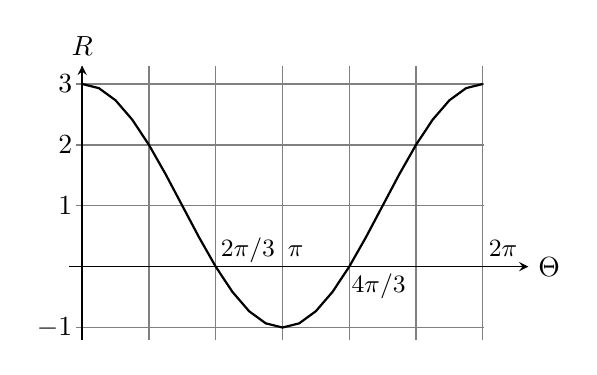
\begin{tikzpicture}[x=2.3038em,y=2.2em]
\pgfsetlinewidth{.5pt}
\pgfsetcolor{gray}
\pgfpathgrid[step={\pgfpointxy{1.0472}{1}}]%
{\pgfpointxy{-.1}{-1.2}}{\pgfpointxy{6.3}{3.3}}
\pgfusepath{stroke}
\pgfsetcolor{black}
%\draw[very thin,stepy=1] (-.2,-1.2) grid (6,3.3);
\draw[-stealth] (-.2,0) -- (7,0) node[right] {$\Theta$}; 
\draw[-stealth] (0,-1.2) -- (0,3.3) node[above] {$R$};
\draw[thick,domain=0:2*pi]
plot (\x,{1+2*cos(\x r)});
\draw (0,-1) node[left] {$-1$};
\draw (0,1) node[left] {$1$};
\draw (0,2) node[left] {$2$};
\draw (0,3) node[left] {$3$};
\draw (2.6,-.1) node[above] {\small $2\pi/3$};
\draw (3.35,0) node[above] {\small $\pi$};
\draw (4.65,.05) node[below] {\small $4\pi/3$};
\draw (6.6,0) node[above] {\small $2\pi$};
\end{tikzpicture}} \\[2em]
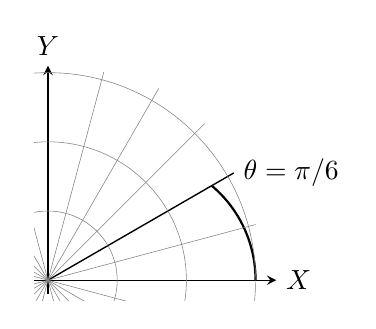
\begin{tikzpicture}[x=2.5em,y=2.5em]
\pgfsetlinewidth{.5pt}
\draw[-stealth] (-.2,0) -- (3.3,0) node[right] {$X$}; 
\draw[-stealth] (0,-.2) -- (0,3.1) node[above] {$Y$};
\draw[thick,domain=0:pi/6]
plot[samples=100] ({cos(\x r)+2*cos(\x r)*cos(\x r)},{sin(\x r)+2*cos(\x r)*sin(\x r)});
\draw (0,0) -- (30:3.1) node[right] {$\theta=\pi/6$};
%
% mallado polar
\clip (-.2,-.3) rectangle (3,3);
\foreach \radio in {1,2,3}
\draw[very thin,color=gray] (0,0) circle (\radio);
%
\foreach \angulo in {15,45,60,75,105,120,135,150,165,%
195,210,225,240,255,285,300,315,330,345}
\draw[very thin,color=gray] (0,0) -- (\angulo:3.2);
\end{tikzpicture} &
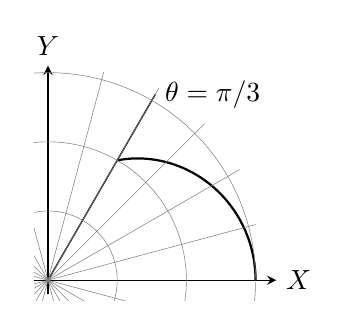
\begin{tikzpicture}[x=2.5em,y=2.5em]
\pgfsetlinewidth{.5pt}
\draw[-stealth] (-.2,0) -- (3.3,0) node[right] {$X$}; 
\draw[-stealth] (0,-.2) -- (0,3.1) node[above] {$Y$};
\draw[thick,domain=0:pi/3]
plot[samples=100] ({cos(\x r)+2*cos(\x r)*cos(\x r)},{sin(\x r)+2*cos(\x r)*sin(\x r)});
\draw (0,0) -- (60:3.1) node[right] {$\theta=\pi/3$};
%
% mallado polar
\clip (-.2,-.3) rectangle (3,3);
\foreach \radio in {1,2,3}
\draw[very thin,color=gray] (0,0) circle (\radio);
%
\foreach \angulo in {15,30,45,60,75,105,120,135,150,165,%
195,210,225,240,255,285,300,315,330,345}
\draw[very thin,color=gray] (0,0) -- (\angulo:3.2);
\end{tikzpicture} \\[2em]
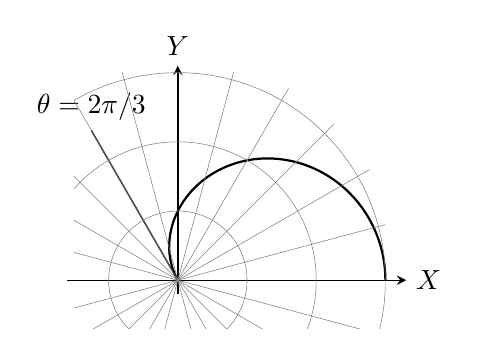
\begin{tikzpicture}[x=2.5em,y=2.5em]
\pgfsetlinewidth{.5pt}
\draw[-stealth] (-1.6,0) -- (3.3,0) node[right] {$X$}; 
\draw[-stealth] (0,-.2) -- (0,3.1) node[above] {$Y$};
\draw[thick,domain=0:2*pi/3]
plot[samples=100] ({cos(\x r)+2*cos(\x r)*cos(\x r)},{sin(\x r)+2*cos(\x r)*sin(\x r)});
\draw (0,0) -- (120:2.5) node[above] {$\theta=2\pi/3$};
%
% mallado polar
\clip (-1.5,-.7) rectangle (3,3);
\foreach \radio in {1,2,3}
\draw[very thin,color=gray] (0,0) circle (\radio);
%
\foreach \angulo in {15,30,45,60,75,105,120,135,150,165,%
195,210,225,240,255,285,300,315,330,345}
\draw[very thin,color=gray] (0,0) -- (\angulo:3.2);
\end{tikzpicture} &
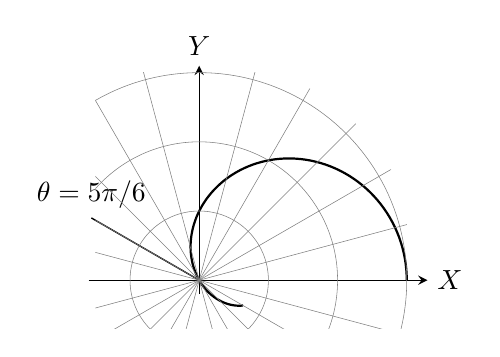
\begin{tikzpicture}[x=2.5em,y=2.5em]
\pgfsetlinewidth{.5pt}
\draw[-stealth] (-1.6,0) -- (3.3,0) node[right] {$X$}; 
\draw[-stealth] (0,-.2) -- (0,3.1) node[above] {$Y$};
\draw[thick,domain=0:5*pi/6]
plot[samples=100] ({cos(\x r)+2*cos(\x r)*cos(\x r)},{sin(\x r)+2*cos(\x r)*sin(\x r)});
\draw (0,0) -- (150:1.8) node[above] {$\theta=5\pi/6$};
%
% mallado polar
\clip (-1.5,-.7) rectangle (3,3);
\foreach \radio in {1,2,3}
\draw[very thin,color=gray] (0,0) circle (\radio);
%
\foreach \angulo in {15,30,45,60,75,105,120,135,150,165,%
195,210,225,240,255,285,300,315,330,345}
\draw[very thin,color=gray] (0,0) -- (\angulo:3.2);
\end{tikzpicture} \\[2em]
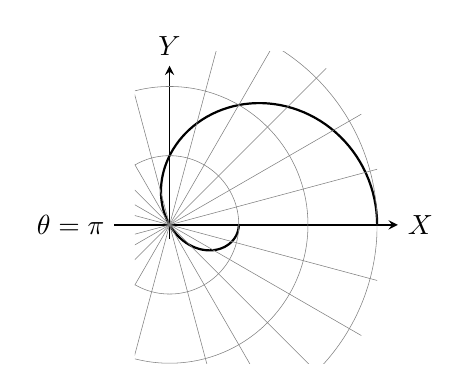
\begin{tikzpicture}[x=2.5em,y=2.5em]
\pgfsetlinewidth{.5pt}
\draw[-stealth] (-.8,0) node[left] {$\theta=\pi$} -- (3.3,0) node[right] {$X$}; 
\draw[-stealth] (0,-.2) -- (0,2.3) node[above] {$Y$};
\draw[thick,domain=0:pi]
plot[samples=100] ({cos(\x r)+2*cos(\x r)*cos(\x r)},{sin(\x r)+2*cos(\x r)*sin(\x r)});
%\draw (0,0) -- (150:2) node[above] {$\theta=5\pi/6$};
%
% mallado polar
\clip (-.5,-2) rectangle (3,2.5);
\foreach \radio in {1,2,3}
\draw[very thin,color=gray] (0,0) circle (\radio);
%
\foreach \angulo in {15,30,45,60,75,105,120,135,150,165,%
195,210,225,240,255,285,300,315,330,345}
\draw[very thin,color=gray] (0,0) -- (\angulo:3.2);
\end{tikzpicture} &
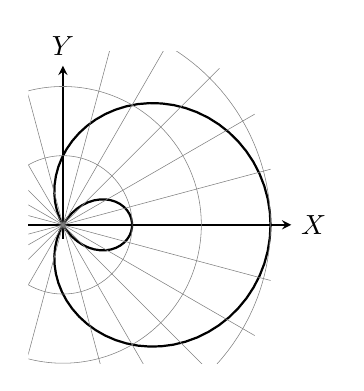
\begin{tikzpicture}[x=2.5em,y=2.5em]
\pgfsetlinewidth{.5pt}
\draw[-stealth] (-.5,0) -- (3.3,0) node[right] {$X$}; 
\draw[-stealth] (0,-.2) -- (0,2.3) node[above] {$Y$};
\draw[thick,domain=0:2*pi]
plot[samples=100] ({cos(\x r)+2*cos(\x r)*cos(\x r)},{sin(\x r)+2*cos(\x r)*sin(\x r)});
%
% mallado polar
\clip (-.5,-2) rectangle (3,2.5);
\foreach \radio in {1,2,3}
\draw[very thin,color=gray] (0,0) circle (\radio);
%
\foreach \angulo in {15,30,45,60,75,105,120,135,150,165,%
195,210,225,240,255,285,300,315,330,345}
\draw[very thin,color=gray] (0,0) -- (\angulo:3.2);
\end{tikzpicture}
\end{tabular}
\end{center}
%\begin{center}
%\includegraphics{caracol1_c.pdf}\\
%%\end{center}
%%%\begin{figure}[p]
%%\begin{center}
%\includegraphics{caracol1_p.pdf}
%\end{center}
\label{caracol}
\caption{Representación de la curva polar $r=1+2\cos\theta$ (Ejemplo~\ref{ej:caracol})}
\end{figure}
\begin{ejemplo}\label{ej:caracol}
Vamos a dibujar la curva polar $r=1+2\cos\theta$, $\theta\in[0,2\pi]$.
La parametrización de esta curva es:
\[
\begin{cases}
& X=(1+2\cos\theta)\cos\theta \\
& Y=(1+2\cos\theta)\operatorname{sen}\theta
\end{cases}
\]
Pero en lugar de usarla para dibujar la curva, vamos a representar primero la función en el plano cartesiano y a trasladar la gráfica al plano polar usando las propiedades establecidas en los resultados anteriores, según se muestra en la página~\pageref{caracol}.

En primer lugar, dibujamos sobre los ejes de coordenadas un ``mallado polar'' sobre el que dibujaremos la curva. Esta malla es similar a la cuadrícula que dibujamos en el plano cartesiano y que nos sirve de referencia; pero en este caso, la malla está formada por rectas radiales correspondientes a ángulos significativos y circunferencias centradas en el origen con diferentes radios.

Podemos observar que para $\theta\in\big(\frac{2\pi}3,\frac{4\pi}3\big)$, $f(\theta)\le0$, por lo que los puntos correspondiente quedan entre el primer y cuarto cuadrante.
Además, $f\big(\frac{2\pi}3\big)=0$, por lo que la recta tangente en el correspondiente punto de la curva es la recta radial de ángulo $\frac{2\pi}3$.
Lo mismo ocurre en $\theta=\frac{4\pi}3$\fej
%\newline
%\rule{0pt}{0pt}
\end{ejemplo}

%:1718 añadir explicación de asíntotas en polares.

\begin{rawhtml}
<p style="text-align: center;"><a href="https://informatica.cv.uma.es/brokenfile.php#/47048/user/draft/78484324/Cartesian_to_polar.gif"><img src="https://informatica.cv.uma.es/brokenfile.php#/47048/user/draft/69143078/Cartesian_to_polar.gif" alt="Cartesian_to_polar.gif" width="300" height="300" style="" class="img-responsive"></a></p>
\end{rawhtml}



\subsection{Cónicas}

Una forma alternativa de describir \emph{lugares geométricos} del plano es mediante \emph{ecuaciones cartesianas}.
Si $P(x,y)$ es cualquier expresión en la que aparecen involucradas las variables $x$ e $y$, la igualdad $P(x,y)=0$ se denomina ecuación cartesiana del siguiente conjunto de puntos:
\[
\{(x,y)\in\mathbb{R}^2\mid P(x,y)=0\}
\]
Dependiendo de la expresión, este conjunto puede ser vacío, contener un único punto o un conjunto finito de puntos, describir una o varias rectas, una o varias curvas e incluso una región del plano.
Para abreviar, en muchas ocasiones nos referiremos al conjunto anterior como ``la curva $P(x,y)=0$''.
% en lugar de ``consideremos la región $C=\{ (x,y)\in\mathbb{R}^2\mid P(x,y)=0\}$''.
%
\begin{ejemplo}
Si $P(x,y)$ es un polinomio de grado uno, entonces $P(x,y)=0$ es una recta.
Por ejemplo, $x-2y-3=0$ describe una recta, de la cual sabemos que el vector $(1,-2)$ es un vector perpendicular a ella, es decir, $(2,1)$ es un \emph{vector director};
sustituyendo $x$ por un valor cualquiera, obtenemos un punto de la recta: para $x=0$, $-2y-3=0$, es decir, $(0,-3/2)$ es un punto de la recta. A partir de aquí, deducimos fácilmente una parametrización:
\begin{equation}
(X,Y)=\left(0,\frac{-3}2\right)+t(2,1)=\left(2t,t-\frac32\right)\tag*{\fej}
\end{equation}
\end{ejemplo}

En esta sección, nos vamos a centrar en las ecuaciones cartesianas definidas por un polinomio de grado dos en las variables $x$ e $y$:
%
\begin{equation}
P(x,y)= ax^2+bxy+cy^2 + \mathit{d}x+\mathit{e}y+f = 0\label{pol}
\end{equation}
%
Para que el polinomio en~\eqref{pol} tenga grado 2, necesariamente al menos uno de los coeficientes $a$, $b$ o $c$ tiene que ser distinto de cero;
en tal caso, el lugar geométrico %es una curva y
se denomina \emph{cónica}.
También están incluidos algunos lugares geométricos que visualmente no son curvas propiamente dichas y que se denominan \emph{cónicas degeneradas}; en el siguiente ejemplo mostramos ejemplos sencillos de este tipo de cónicas.
%
\begin{ejemplo-br}
\begin{enumerate}
\item
$\{(x,y)\mid x^2+y^2+1=0\}=\varnothing$
\item
$\{(x,y)\mid x^2+y^2=0\}=(0,0)$
\item
$\{(x,y)\mid x^2-y^2=0\}$ está formado por las rectas $x+y=0$, $x-y=0$
\fej
\end{enumerate}
\end{ejemplo-br}
%
En este curso, vamos a trabajar con los polinomios de grado 2 sin término en $xy$.
Aparte de los tres casos del ejemplo anterior, si $b=0$ la ecuación~\eqref{pol} puede definir una de las cuatro curvas que presentamos en los apartados siguientes.

\begin{rawhtml}
<p style="text-align: center;"><iframe width="560" height="316" src="https://www.youtube.com/embed/gy6olKwCo-Y?list=PL2rtpLKW91qaoiK4EarXJ63UTuWldV2ul" frameborder="0" allowfullscreen=""></iframe></p>
\end{rawhtml}

\paragraph{Circunferencia.}
El lugar geométrico de los puntos cuya distancia a un punto fijo $C=(x_0,y_0)$ es
constantemente $r>0$, se denomina \emph{circunferencia de centro $C$ y radio $r$} y su ecuación cartesiana es:
\begin{center}
\begin{tabular}{c@{\qquad}c}
$(x-x_0)^2+(y-y_0)^2=r^2$ &
\raisebox{-4.5em}{
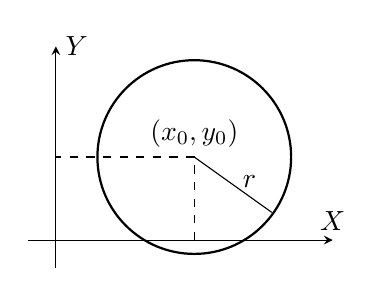
\begin{tikzpicture}[x=1em,y=1em]
%\pgfsetlinewidth{.5pt}
\draw[-stealth] (-1,0) -- (10,0) node[above] {$X$}; 
\draw[-stealth] (0,-1) -- (0,7) node[right] {$Y$};
\draw[dashed] (5,0) -- (5,3) -- (0,3);
\draw[thick] (5,3) circle (3.5); 
\draw (5,3) -- (7.8,1);
\draw (5,3) node[above] {$(x_0,y_0)$};
\draw (7,2.1) node {$r$};
\end{tikzpicture}
%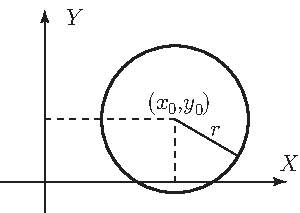
\includegraphics{T2/figs/circunferencia.pdf}
}
\end{tabular}
\end{center}

La circunferencia es un caso particular de elipse, que definimos en el ítem siguiente, aunque por su importancia, la destacamos como un tipo distinto.
%
\begin{ejemplo}
La ecuación 
$x^2+y^2=4$ determina una circunferencia centrada en el origen y de radio 2.
Si con el mismo radio, queremos que esté centrada en $(-1,2)$, la ecuación será:
\begin{equation}
(x+1)^2+(y-2)^2=4\qquad\Longleftrightarrow\qquad
x^2+y^2+2x-4y+1=0\tag*{\fej}
\end{equation}
\end{ejemplo}
%
Observamos en este ejemplo que, al desarrollar los cuadrados, el polinomio no tiene término en $xy$ y los coeficientes en $x^2$ e $y^2$ son iguales; de hecho, podemos caracterizar a las circunferencias como sigue:
\emph{si $b=0$ y $a=c$, entonces la ecuación~\ref{pol} representa una circunferencia o una cónica degenerada}. Para deducir si es degenerada u obtener el centro y el radio de la circunferencia, basta con aplicar la técnica de completar cuadrados a los sumandos en $x$ y a los sumandos en $y$.
%
\begin{ejemplo}
La ecuación $9x^2+9y^2-36x+54y+116=0$ corresponde a una circunferencia:
\begin{multline*}
0=9x^2+9y^2-36x+54y+116=
9(x-2)^2+9(y+3)^2-1\Longleftrightarrow\\
\Longleftrightarrow (x-2)^2+(y+3)^2=\frac19
\end{multline*}
Es decir, su centro es $(2,-3)$ y su radio es $1/3$.
\fej
\end{ejemplo}
\paragraph{Elipse.}
%Consideremos dos puntos $F_1$ y $F_2$;
El lugar geométrico de los puntos cuya suma de distancias a dos puntos $F_1$ y $F_2$ es constante se denomina \emph{elipse}.
El \emph{centro} de la elipse es el punto medio del segmento que une los dos focos, es decir, $\frac12(F_1+F_2)$. 
Si los focos están en los puntos $(-c,0)$ y
$(c,0)$, con $c>0$, y la suma de las distancias a los focos es $2a$, la ecuación queda como sigue:
\begin{center}
\begin{tabular}{c@{\qquad}c}
$\dfrac{x^2}{a^2}+\dfrac{y^2}{b^2}=1$ &
\raisebox{-4.5em}{
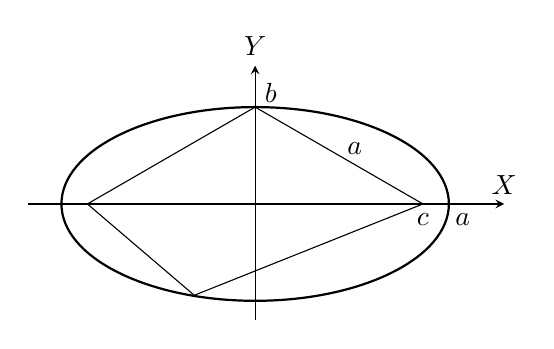
\begin{tikzpicture}[x=1em,y=1em]
%\pgfsetlinewidth{.5pt}
\draw[-stealth] (-8.2,0) -- (9,0) node[above] {$X$}; 
\draw[-stealth] (0,-4.2) -- (0,5) node[above] {$Y$};
\draw[thick] (0,0) ellipse (7 and 3.5); 
\draw (-6.062177826491,0) -- (0,3.5) -- (6.062177826491,0);
\draw (-6.062177826491,0) -- (-2.2,-3.3) -- (6.062177826491,0);
\draw (0,4) node[right] {$b$};
\draw (6.062177826491,0) node[below] {$c$};
\draw (3.6,2) node {$a$};
\draw (7.5,0) node[below] {$a$};
%\draw (5,3) -- (7.8,1);
%\draw (5,3) node[above] {$(x_0,y_0)$};
%\draw (7,2.1) node {$r$};
\end{tikzpicture}
%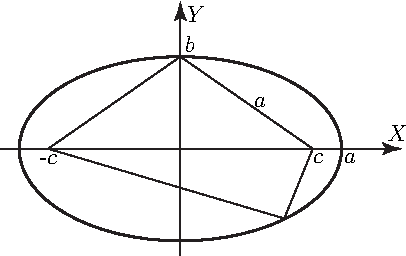
\includegraphics{T2/figs/elipse.pdf}
}
\end{tabular}
\end{center}
verificándose que $a^2=c^2+b^2$, por lo que, necesariamente, $a>b$.

Si los focos están en los puntos $(0,-c)$ y
$(0,c)$, con $c>0$, y la suma de las distancias a los focos es $2b$, la ecuación que se obtiene es la misma,
\begin{center}
\begin{tabular}{c@{\qquad}c}
$\dfrac{x^2}{a^2}+\dfrac{y^2}{b^2}=1$ &
\raisebox{-4.5em}{
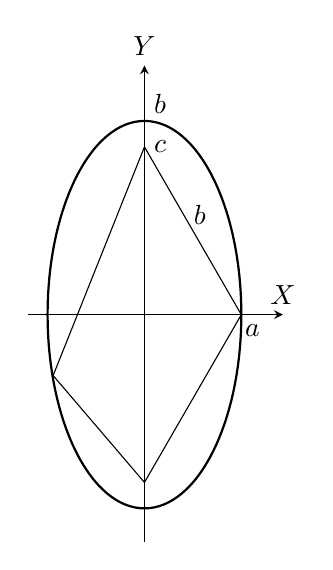
\begin{tikzpicture}[x=1em,y=1em]
%\pgfsetlinewidth{.5pt}
\draw[-stealth] (0,-8.2) -- (0,9) node[above] {$Y$}; 
\draw[-stealth] (-4.2,0) -- (5,0) node[above] {$X$};
\draw[thick] (0,0) ellipse (3.5 and 7); 
\draw (0,-6.062177826491) -- (3.5,0) -- (0,6.062177826491);
\draw (0,-6.062177826491) -- (-3.3,-2.2) -- (0,6.062177826491);
\draw (3.9,0) node[below] {$a$};
\draw (0,6.062177826491) node[right] {$c$};
\draw (2,3.6) node {$b$};
\draw (0,7.6) node[right] {$b$};
%\draw (5,3) -- (7.8,1);
%\draw (5,3) node[above] {$(x_0,y_0)$};
%\draw (7,2.1) node {$r$};
\end{tikzpicture}
%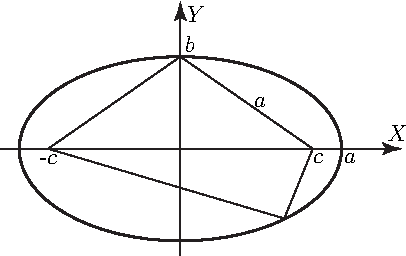
\includegraphics{T2/figs/elipse.pdf}
}
\end{tabular}
\end{center}
verificándose la igualdad $b^2=c^2+a^2$, por lo que necesariamente $b>a$.

Si desplazamos la elipse para que tenga su centro en $(x_0,y_0)$, la ecuación que obtenemos es
\[
\dfrac{(x-x_0)^2}{a^2}+\dfrac{(y-y_0)^2}{b^2}=1
\]
Si desarrollamos los cuadrados, obtendremos un polinomio sin término en $xy$, aunque en este caso los coeficientes de $x^2$ e $y^2$ son distintos pero con el mismo signo.

%:1718 añadir ejemplos de elipse, hipérbola y parábola
% igual que hemos hecho con la circunferencia


\paragraph{Hipérbola.}
El lugar geométrico de los puntos cuya
diferencia de distancias a dos puntos $F_1$ y $F_2$ es constante se denomina \emph{hipérbola}.
El \emph{centro} de la hipérbola es el punto medio del segmento que une los dos focos, es decir, $\frac12(F_1+F_2)$. 
Si los focos están en los puntos $(-c,0)$ y $(c,0)$, con $c>0$, y $2a$ es la diferencia de las distancias a los focos, la ecuación de la hipérbola es
\begin{center} 
\begin{tabular}{c@{\qquad}c}
$\dfrac{x^2}{a^2}-\dfrac{y^2}{b^2}=1$ & 
\raisebox{-6.8em}{
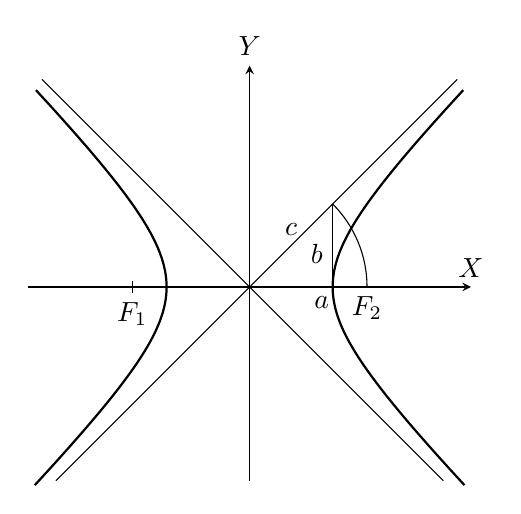
\begin{tikzpicture}[x=1em,y=1em]
%\pgfsetlinewidth{.5pt}
\draw[-stealth] (-8,0) -- (8,0) node[above] {$X$}; 
\draw[-stealth] (0,-7) -- (0,8) node[above] {$Y$};
%
\draw (-7,-7) -- (7.5,7.5);
\draw (-7.5,7.5) -- (7,-7);
\draw[thick,domain=-.028:.028]
plot[samples=100] ({3*cosh(\x r)},{3*sinh(\x r)});
\draw[thick,domain=-.028:.028]
plot[samples=100] ({-3*cosh(\x r)},{3*sinh(\x r)});
%
\draw (3,0) -- (3,3);
\draw (3,1.2) node[left] {$b$};
\draw (2.6,0) node[below] {$a$};
\draw (1.5,1.5) node[above] {$c$};
\draw (4.242640687119,0) node[below] {$F_2$};
\draw (-4.242640687119,.2) -- (-4.242640687119,-.2) node[below] {$F_1$};
\draw (0,0) +(0:4.242640687119) arc (0:45:4.242640687119);
\end{tikzpicture}
%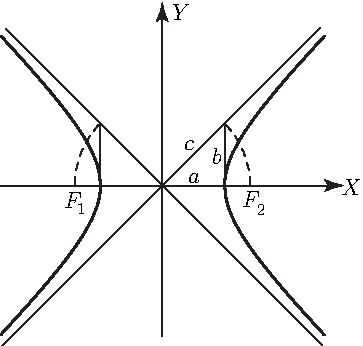
\includegraphics{T2/figs/hiperbola1.pdf}
}
\end{tabular}
\end{center}
en donde $a^2+b^2=c^2$.
Si los focos están en los puntos $(0,-c)$ y $(0,c)$, con $c>0$, y $2b$ es la diferencia de las distancias a los focos, la ecuación de la hipérbola es
\begin{center} 
\begin{tabular}{c@{\qquad}c}
$\dfrac{-x^2}{a^2}+\dfrac{y^2}{b^2}=1$ &
\raisebox{-6.8em}{
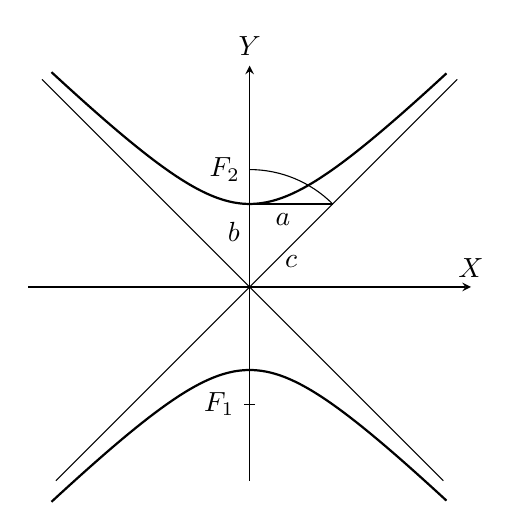
\begin{tikzpicture}[x=1em,y=1em]
%\pgfsetlinewidth{.5pt}
\draw[-stealth] (-8,0) -- (8,0) node[above] {$X$}; 
\draw[-stealth] (0,-7) -- (0,8) node[above] {$Y$};
%
%:AQUI
\draw (-7,-7) -- (7.5,7.5);
\draw (-7.5,7.5) -- (7,-7);
\draw[thick,domain=-.028:.028]
plot[samples=100] ({3*sinh(\x r)},{3*cosh(\x r)});
\draw[thick,domain=-.028:.028]
plot[samples=100] ({3*sinh(\x r)},{-3*cosh(\x r)});
%
\draw (0,3) -- (3,3);
\draw (1.2,3) node[below] {$a$};
\draw (0,2) node[left] {$b$};
\draw (1.5,1.5) node[below] {$c$};
\draw (0,4.242640687119) node[left] {$F_2$};
\draw (.2,-4.242640687119) -- (-.2,-4.242640687119) node[left] {$F_1$};
\draw (0,0) +(45:4.242640687119) arc (45:90:4.242640687119);
\end{tikzpicture}
%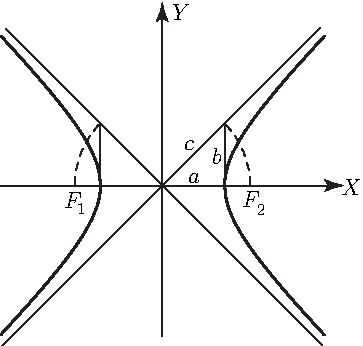
\includegraphics{T2/figs/hiperbola1.pdf}
}
\end{tabular}
\end{center}

en donde igualmente $a^2+b^2=c^2$.
Como se observa en las figuras, en ambos casos las rectas $bx-ay=0$, $bx+ay=0$ están muy próximas a la curva pero no la cortan; estas rectas son las \emph{asíntotas} de la hipérbolas. 

Si desplazamos las hipérbolas para que tengan su centro en $(x_0,y_0)$, las ecuaciones que obtenemos son
\[
\dfrac{(x-x_0)^2}{a^2}-\dfrac{(y-y_0)^2}{b^2}=1\qquad\quad
\dfrac{-(x-x_0)^2}{a^2}+\dfrac{(y-y_0)^2}{b^2}=1
\]
%\enlargethispage{1.5\baselineskip}
Si desarrollamos los cuadrados, obtendremos polinomios sin término en $xy$ y los coeficientes de $x^2$ e $y^2$ tienen distinto signo.

\paragraph{Parábola.}
El lugar geométrico de los puntos que equidistan de una recta $r$ y un punto $F$, se denomina \emph{parábola con foco $F$ y directriz $r$}.
En la figura que aparece abajo, mostramos dos ejemplos de parábolas;
si el foco es el punto $(0,\mathit{d})$ y la directriz es $y=-\mathit{d}$, obtenemos la parábola de la izquierda;
si el foco es el punto $(\mathit{d},0)$ y la directriz es $x=-\mathit{d}$, obtenemos la parábola de la derecha:

\begin{center}
\begin{tabular}{c@{\qquad\qquad}c}
$x^2=4\mathit{d}y$ & $y^2=4\mathit{d}x$ \\[.5em]
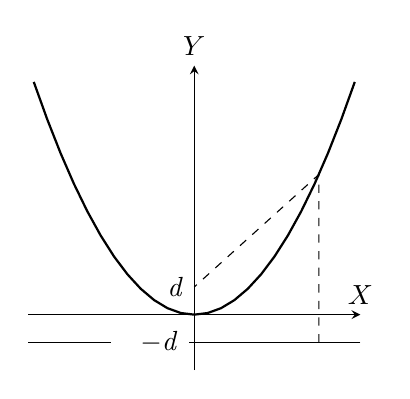
\begin{tikzpicture}[x=1em,y=1em]
%\pgfsetlinewidth{.5pt}
\draw[-stealth] (-6,0) -- (6,0) node[above] {$X$}; 
\draw[-stealth] (0,-2) -- (0,9) node[above] {$Y$};
%!TEX encoding = UTF-8 Unicode
\draw[%color=blue,
thick,domain=-5.8:5.8]
plot (\x,.25*\x*\x);
%
\draw (-6,-1) -- (-3,-1);
\draw (6,-1) -- (-.2,-1) node[left] {$-\mathit{d}$};
\draw[dashed]  (4.5,-1) -- (4.5,5.0625) --(0,1) node[left] {$\mathit{d}$};
\end{tikzpicture}
&
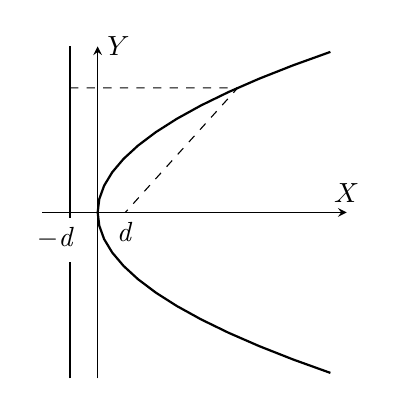
\begin{tikzpicture}[x=1em,y=1em]
%\pgfsetlinewidth{.5pt}
\draw[-stealth] (0,-6) -- (0,6) node[right] {$Y$}; 
\draw[-stealth] (-2,0) -- (9,0) node[above] {$X$};
%
\draw[%color=blue,
thick,domain=-5.8:5.8]
plot (.25*\x*\x,\x);
%
\draw (-1,-6) -- (-1,-1.8);
\draw (-1,6) -- (-1,-.2);
\draw (-1.5,-.2) node[below] {$-\mathit{d}$};
\draw[dashed]  (-1,4.5) -- (5.0625,4.5) --(1,0) node[below] {$\mathit{d}$};
\end{tikzpicture}
\end{tabular}
\end{center}

Si desplazamos estas parábolas para que tengan su vértice en $(x_0,y_0)$, las ecuaciones  que obtenemos son:
\[
(x-x_0)^2=4\mathit{d}(y-y_0),\hspace{5em} (y-y_0)^2=4\mathit{d}(x-x_0)
\]
Al desarrollar estas ecuaciones obtenemos polinomios en los que no hay término en $xy$ y falta, o bien el término en $x^2$, o bien el término en $y^2$.

\begin{rawhtml}
<p style="text-align: center;"><iframe width="560" height="316" src="https://www.youtube.com/embed/yk95zU_1B4I?list=PL2rtpLKW91qaoiK4EarXJ63UTuWldV2ul" frameborder="0" allowfullscreen=""></iframe></p>
\end{rawhtml}

Otra forma de obtener estas curvas es mediante la siguiente descripción.
Si consideramos un cono circular hueco y lo cortamos con un plano, la curva resultante en la
sección es una \emph{cónica} y
dependiendo del ángulo de corte, se obtiene una u otra.
%
%\enlargethispage{\baselineskip}
\begin{center}
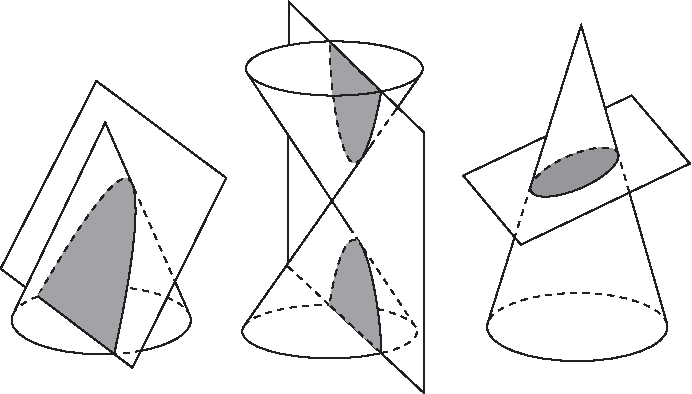
\includegraphics{T2/figs/conicas.pdf}\\
Parábola\qquad\qquad\qquad\qquad Hipérbola\qquad\qquad\qquad\qquad Elipse
\end{center}
%
Si el corte es perpendicular al eje de cono, obtenemos una circunferencia; si el corte es paralelo a la generatriz se obtiene una parábola; si el corte es paralelo al eje se obtiene una hipérbola; cualquier otro corte, produce una elipse.

Naturalmente, también es posible describir una cónica mediante ecuaciones paramétricas.
A continuación vemos la parametrizaciones de las cónicas en sus posiciones \emph{típicas} y en la sección siguiente aprenderemos cómo parametrizar una cónica arbitraria.
%
\label{pag:con-tipicas}
%
\begin{description}
\item[Circunferencia]
con centro $(x_0,y_0)$ y radio $r$:
\[
(x-x_0)^2+(y-y_0)^2=r^2 \qquad\qquad
\begin{cases}
& x(t)= x_0 + r \cos t\\
& y(t)= y_0 + r \operatorname{sen} t\\
& t\in[0,2\pi]
\end{cases}\]
\item[Elipse]
centrada en $(x_0,y_0)$ y semiejes $a>0$ y $b>0$:
\[
\frac{(x-x_0)^2}{a^2}+\frac{(y-y_0)^2}{b^2}=1 \qquad\qquad\begin{cases}
& x(t)= x_0 + a \cos t\\
& y(t)= y_0 + b\operatorname{sen} t\\
& t \in[0,2\pi]
\end{cases}\]

\item[Hipérbola] centrada $(x_0,y_0)$,
con asíntotas paralelas a las rectas $bx+ay=0$,\newline
$bx-ay=0$, $a>0$, $b>0$, y cortando al eje $OX$:
\[
\frac{(x-x_0)^2}{a^2}-\frac{(y-y_0)^2}{b^2}=1, \quad\begin{cases}
& x(t)= x_0+a \cosh t\\
& y(t)= y_0+b \operatorname{senh} t\\
& t\in\mathbb{R}
\end{cases}\quad
\begin{cases}
& x(t)= x_0-a \cosh t\\
& y(t)= y_0+b \operatorname{senh} t\\
& t\in\mathbb{R}
\end{cases}\]
Centrada $(x_0,y_0)$, con asíntotas paralelas a las rectas $bx+ay=0$, $bx-ay=0$, $a>0$, $b>0$, y cortando al eje $OY$:
\[
\frac{-(x-x_0)^2}{a^2}+\frac{(y-y_0)^2}{b^2}=1, \quad\begin{cases}
& x(t)= x_0+a \operatorname{senh} t\\
& y(t)= y_0+b \cosh t\\
& t\in\mathbb{R}
\end{cases}\quad
\begin{cases}
& x(t)= x_0+a \operatorname{senh} t\\
& y(t)= y_0-b \cosh t\\
& t\in\mathbb{R}
\end{cases}\]

En estos casos, necesitamos una parametrización distinta para cada rama de la hipérbola.

\item[Parábola] con vértice en $(x_0,y_0)$, eje paralelo a $OY$, $\frac a4>0$ distancia del foco al vértice:
\[
(x-x_0)^2=a(y-y_0)
\qquad\begin{cases}
& x(t)= x_0+a\cdot t \\
& y(t)= y_0+a\cdot t^2\\
& t\in\mathbb{R}
\end{cases}
\]
Con vértice en $(x_0,y_0)$, eje paralelo a $OX$, $\frac a4>0$ distancia del foco al vértice:
\[
(y-y_0)^2=a(x-x_0)\qquad
\begin{cases}
& x(t)= x_0+a\cdot t^2\\
& y(t)= y_0+a\cdot t \\
& t\in\mathbb{R}
\end{cases}
\]

\end{description}

\begin{rawhtml}
<p style="text-align: center;"><iframe width="560" height="316" src="https://www.youtube.com/embed/JEzrPUp6k4s?list=PL2rtpLKW91qaoiK4EarXJ63UTuWldV2ul" frameborder="0" allowfullscreen=""></iframe></p>
\end{rawhtml}

%\newpage
%\thispagestyle{empty}
%
%\ 

\newpage


\section{Campos escalares}

En la lección anterior hemos trabajado con polinomios de dos variables, es decir, un ejemplo de función definida en el espacio $\mathbb{R}^2$.
En esta lección, vamos a trabajar con funciones generales con dos o más variables, es decir, vamos a trabajar con funciones definidas en espacios $\mathbb{R}^m$.
Posiblemente, se haya trabajado en estos espacios utilizando su estructura de \emph{espacio vectorial} pero ahora, estamos interesados en establecer las nociones de \emph{continuidad} y
\emph{diferenciabilidad} de funciones definidas en ellos.

Para denotar los elementos de $\mathbb{R}^m$ se suele utilizar una variable con un flecha encima, $\vec{x}$, o bien variables en ``negrita'', $\boldsymbol{x}$;
a lo largo del curso utilizaremos esta segunda notación, ya que los elementos de $\mathbb{R}^m$ pueden identificarse tanto con vectores como con puntos.
Además, escribiremos las coordenadas de los vectores utilizando subíndices:
$\boldsymbol{x}=(x_1,\dots,x_m)\in\mathbb{R}^m$.

En general, cualquier función definida en un subconjunto de un espacio $\mathbb{R}^m$ se denomina
\emph{función de varias variables}.
Si la imagen está contenida en $\mathbb{R}$ se denomina \emph{campo escalar},
\[
f\colon \mathit{D}\subset \mathbb{R}^m\to\mathbb{R}
\]
Si la imagen está contenida en $\mathbb{R}^k$ se denomina \emph{campo vectorial},
\[
f\colon \mathit{D}\subset \mathbb{R}^m\to\mathbb{R}^k
\]
En este tema, nos centramos en los campos escalares, en la lección anterior hemos trabajado con funciones vectoriales y, más adelante en el curso, trabajaremos con campos vectoriales.
En cualquiera de los dos casos, el conjunto $\mathit{D}$ se denomina \emph{dominio} del campo y se denota $\mathrm{Dom}(f)$.
Algunos problemas exigirán trabajar en un dominio determinado y en tal caso tendrá que ser especificado;
en caso contrario, entenderemos que el dominio es el mayor posible.
%
\begin{ejemplo}
La expresión $f(x,y)=\dfrac1{\sqrt{x-y}}$ define un campo de $\mathbb{R}^2$ en $\mathbb{R}$.
El mayor dominio con el que podemos trabajar es el formado por los puntos tales que~$x>y$, es decir:
\[
\mathrm{Dom}(f)=\{(x,y)\in\mathbb{R}^2\mid x>y\}
\]
Gráficamente, los puntos del dominio son los que están estrictamente por debajo de la bisectriz del primer y tercer cuadrante del plano~$\mathbb{R}^2$.\fej
\end{ejemplo}
%
Sabemos que la representación gráfica de las funciones reales de una variable es una herramienta muy útil para describir sus características; sin embargo, en campos escalares solo podremos utilizar esta herramienta en unos pocos casos.
Por una parte, podemos definir el grafo de un campo escalar~$f$ como
%
\[
\mathrm{gr}(f)=\{ (x_1,\dots,x_m,f(x_1,\dots,x_m))\in\mathbb{R}^{m+1};
(x_1,\dots,x_m)\in\mathrm{Dom}(f)\}
\]
aunque solamente podremos visualizar este conjunto para $m=1$ o $m=2$, ya que en tal caso, este conjunto es una superficie de $\mathbb{R}^3$.
%
\begin{ejemplo}
El campo escalar definido por $f(x,y)=x^2+y^2$ tiene por dominio a todo el espacio $\mathbb{R}^2$.
Su grafo es el conjunto:
\[
\mathrm{gr}(f)=\{ (x,y,x^2+y^2); (x,y)\in\mathbb{R}^2\}
\]
No es difícil imaginar cuál es la forma de esta superficie si observamos que, haciendo constante la coordenada $z$ de cada punto, $x^2+y^2=c$, las curvas que obtenemos son circunferencias y si cortamos por cualquier plano que contenga al eje $OZ$, es decir,
$y=mx$, las curvas que obtenemos son parábolas.
Es decir, la superficie es la figura de revolución que se obtiene al girar una parábola sobre su eje.
Esta superficie es la que nos encontramos, por ejemplo, en las antenas parabólicas.\fej
\end{ejemplo}

Otra forma de representar los campos escalares es a través de las \emph{superficies} y \emph{curvas de nivel}:
si $c\in\mathrm{Im}(f)$, llamamos \emph{superficie de nivel} de $f$ asociada a $c$, al conjunto
\[
N(f,c)=\{ \boldsymbol{x}\in \mathit{D}\mid f(\boldsymbol{x})=c\}
\]
Si $m=2$ estos conjuntos se denominan \emph{curvas de nivel}.
Aunque, como hemos visto en la lección anterior, los conjuntos descritos como $f(x,y)=0$ no tienen que ser necesariamente curvas, puede ser un conjunto vacío, contener uno o varios puntos, una o varias rectas o curvas,\dots
%
\begin{figure}
\begin{center}
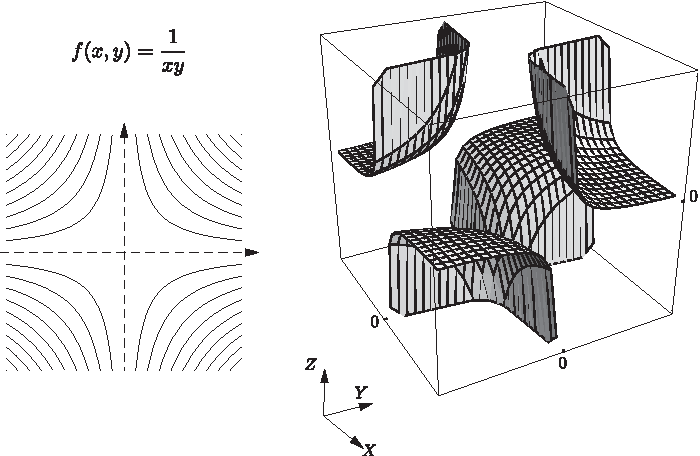
\includegraphics{T2/figs/nivel1.pdf}\\[5em]
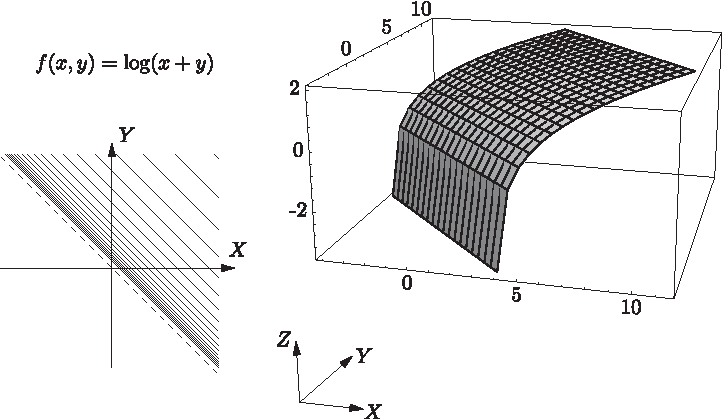
\includegraphics{T2/figs/nivel2.pdf}
\end{center}
\caption{Representación de campos escalares}\label{fig-rep1}
\end{figure}

\begin{figure}
\begin{center}
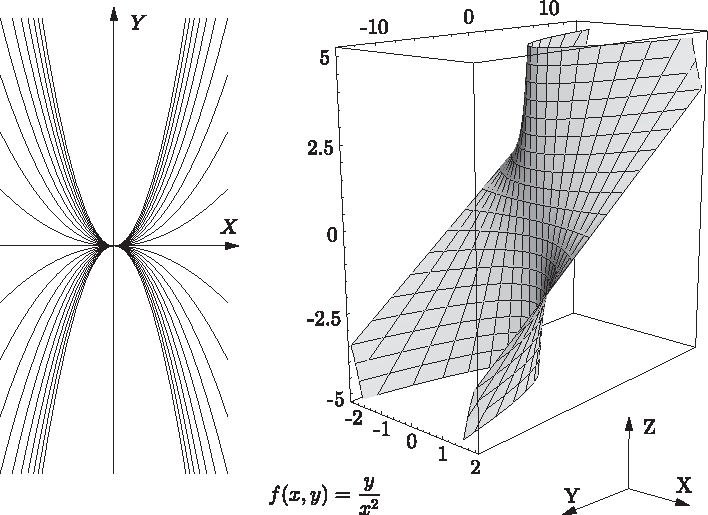
\includegraphics{T2/figs/nivel3.pdf}\\[5em]
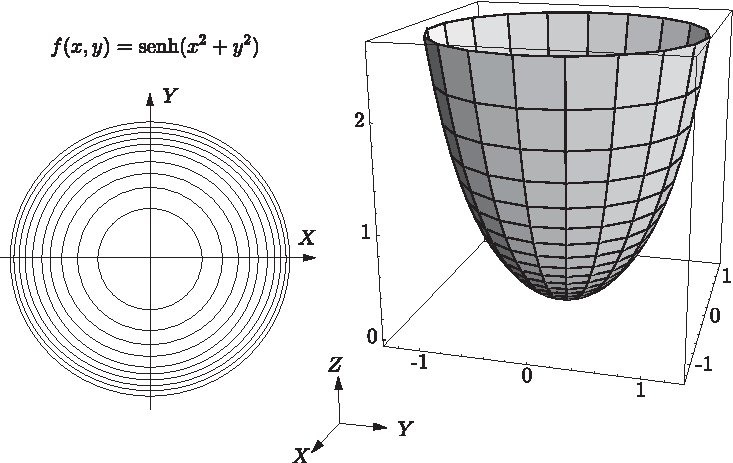
\includegraphics{T2/figs/nivel4.pdf}
\end{center}
\caption{Representación de campos escalares}\label{fig-rep2}
\end{figure}
%
\begin{ejemplo}\label{ej:cn}
En el campo $f(x,y)=x^2+y^2$, las curvas de nivel serían:
\[
x^2+y^2=c,\quad c> 0
\]
Sabemos de la lección anterior que estas curvas son circunferencias centradas en el origen y radio
$\sqrt c$.

El campo $g(x,y)=\log(x^2+y^2)$ tiene las mismas curvas de nivel, circunferencias centradas en el origen:
\begin{align*}
\log(x^2+y^2) &= c\\
x^2+y^2 &=e^c
\end{align*}
Sin embargo, para cada valor $c$, su radio es $\sqrt{e^c}$.\fej
\end{ejemplo}
%
Para poder visualizar los campos usando sus curvas nivel se hace la representación de la siguiente forma:
elegimos varios valores equidistantes, $c_1$, $c_2$,\dots, $c_n$, y dibujamos las curvas correspondientes a estos valores, $f(\boldsymbol{x})=c_i$.
Por ejemplo, aunque los dos campos del ejemplo~\ref{ej:cn}, $f(x,y)=x^2+y^2$, $g(x,y)=\log(x^2+y^2)$, tienen las mismas curvas de nivel, su representación sería distinta, ya que para los mismos valores $c_i$, las circunferencias correspondientes a dichos valores, son distintas.

Podemos encontrar representaciones de campos mediante curvas de nivel en los mapas de temperaturas y de presiones;
en estos casos, las curvas de nivel se denominan isotermas e isobaras respectivamente.
En las figuras~\ref{fig-rep1} y \ref{fig-rep2} vemos algunos ejemplos de campos escalares y sus representaciones haciendo uso del grafo y de curvas de nivel.

\begin{rawhtml}
<p style="text-align: center;"><iframe width="560" height="316" src="https://www.youtube.com/embed/bjOLBj6lLhs?list=PL2rtpLKW91qYfkQ_gzsN2-UGxdfRYJ03_" frameborder="0" allowfullscreen=""></iframe></p>
\end{rawhtml}

\subsection{Campos escalares lineales}\label{sec:lin}

Dedicamos esta sección a un ejemplo de campo escalar: los \emph{campos escalares lineales}.
Estas aplicaciones serán la base para las definiciones y desarrollos asociados al concepto de diferenciabilidad.

Los \emph{campos escalares lineales} en $\mathbb{R}^n$ responden a la expresión:
\[
f(x_1,\dots,x_n) = a_1x_1+\dots+a_nx_n
\]
en donde $a_1$,\dots,$a_n$ son números reales.
La expresión $a_1x_1+\dots+a_nx_n$ se denomina igualmente \emph{forma lineal} y es un polinomio de grado 1 sin término independiente.

Estos campos se pueden escribir de varias formas. Por ejemplo, en forma matricial se definen a partir de la matriz $A=(a_1 \cdots a_n)\in \mathcal{M}_{1\times n}(\mathbb{R})$:
\[
f(x_1,\dots,x_n) = (a_1 \cdots a_n)
\begin{pmatrix}
x_1\\
\vdots\\
x_n
\end{pmatrix}
= A\boldsymbol x
\]
Aunque anteriormente hemos representado los vectores como $(x_1,\dots,x_n)$, cuando trabajamos matricialmente, los vectores deben tratarse como matrices columna:
\[
\boldsymbol x = \begin{pmatrix}
x_1\\
\vdots\\
x_n
\end{pmatrix}
\in \mathcal{M}_{n\times 1}(\mathbb{R})
\]
Para los objetivos de este tema y para los cálculos que realizaremos en él, es más adecuado, sin embargo, definir los campos escalares lineales usando el \emph{producto escalar};
en este caso, el campo escalar lineal se define con el vector $\boldsymbol a=(a_1,\dots, a_n)\in \mathbb{R}^n$:
\[
f(\boldsymbol x) = \boldsymbol a\cdot \boldsymbol x
\]
No obstante, no debemos olvidar que las tres expresiones definen la misma función y que por lo tanto, solo son tres formas distintas de escribir lo mismo.
%
\begin{ejemplo}
El campo $f(x,y,z)=6x-y+2z$ es un campo lineal y se puede escribir como:
\begin{equation}
f(x,y,z)=6x-y+2z=(6,-1,2)\cdot (x,y,z)
\tag*{\fej}
\end{equation}
\end{ejemplo}
%
Recordemos ahora las propiedades más importantes de los campos lineales.
Si $f$ es un campo escalar lineal, entonces:
%:teo:aplin
\begin{teorema}\label{teo:aplin}
Si $f$ es un campo escalar lineal, entonces:\vspace{-1em}
\begin{enumerate}
\item
$f(\boldsymbol x+\boldsymbol y) = f(\boldsymbol x)+f(\boldsymbol y)$ para todo $\boldsymbol x,\boldsymbol y\in\mathbb{R}^n$.
\item
$f(k\boldsymbol x) = kf(\boldsymbol x)$ para todo $\boldsymbol x\in\mathbb{R}^n$ y para todo $k\in\mathbb{R}$.
\item
Si para cada $i$ 
\[
a_i=f(\boldsymbol e_i)=f(0,\dots,\stackrel{i}{\check1},\dots,0)
\]
y $\boldsymbol a=(a_1,\dots,a_n)$, entonces $f(\boldsymbol x)=\boldsymbol a\cdot\boldsymbol x$.
\end{enumerate}
\end{teorema}
%
Las dos primeras propiedades caracterizan a las aplicaciones lineales y son usadas para definir este tipo de aplicaciones en espacios vectoriales generales.
La tercera propiedad se usa fundamentalmente para hacer desarrollos sobre aplicaciones lineales desconocidas o arbitrarias, ya que nos da una forma de expresar los coeficientes a partir de la propia aplicación.

Los campos lineales no deben confundirse con los \emph{campos afines}, que se definen a partir de ellos como sigue.
%
\begin{definicion}
Un campo afín en $\mathbb{R}^n$ responde a la expresión
\[
f(x_1,\dots,x_n) = a_1x_1+\dots+a_nx_n +b
\]
que puede ser escrita haciendo uso del producto escalar como
\[
f(\boldsymbol x) = \boldsymbol a\cdot \boldsymbol x+b
\]
\end{definicion}
%
En el caso particular de $\mathbb{R}^2$, haremos uso de los grafos de los campos lineales y afines.
Concretamente, el grafo del campo $f(x,y)=a_1x+a_2y$ es el plano
\[
a_1x+a_2y-z = 0
\]
que es normal (perpendicular) al vector $(a_1,a_2,-1)$ y pasa por el origen de coordenadas.
De la misma forma, el grafo del campo afín $f(x,y)=a_1x+a_2y+b$ es el plano
\[
a_1x+a_2y-(z-b) = 0
\]
que pasa por el punto $(0,0,b)$ y es normal al vector $(a_1,a_2,-1)$.

A lo largo del tema, trabajaremos con planos en $\mathbb{R}^3$, por lo que es conveniente repasar las distintas formas de expresar analíticamente este tipo de conjuntos.
En particular, para determinar un plano en $\mathbb{R}^3$ es suficiente con dar un punto del plano, $P_0=(x_0,y_0,z_0)$, y un vector normal, $\boldsymbol v=(v_1,v_2,v_3)$; la ecuación del plano dado por estos dos elementos es
\[
v_1(x-x_0)+v_2(y-y_0)+v_3(z-z_0) = 0
\]
Esto es consecuencia de la definición del producto escalar, por la cual, el producto de dos vectores perpendiculares es 0. En este caso, si $P=(x,y,z)$ es cualquier punto del plano, entonces el vector
$\overrightarrow{P_0P}=P-P_0$ es perpendicular al vector $\boldsymbol v$ y por lo tanto:
\begin{align*}
&\boldsymbol v\cdot(P-P_0)=0\\
&(v_1,v_2,v_3)\cdot(x-x_0,y-y_0,z-z_0) = 0\\
&v_1(x-x_0)+v_2(y-y_0)+v_3(z-z_0) = 0
\end{align*}
%
\begin{ejemplo}
%\begin{enumerate}
%\item
%La recta perpendicular al vector $(1,-2)$ y que pasa por el origen de coordendas es:
%\[
%x-2y=0
%\]
%Si queremos que la recta pase por el punto $(0,-1)$, la ecuación es:
%\begin{align*}
%x-2(y+1)&=0\\
%x-2y-2&=0
%\end{align*}
%\item
El plano perpendicular al vector $(-2,1,-1)$ y que pasa por el origen de coordenadas es:
\[
-2x+y-z=0
\]
Si queremos que el plano pase por el punto $(-1,0,1)$, la ecuación es:
\begin{align*}
-2(x+1)+y-(z-1)&=0\\
-2x+y-z -1 &=0\tag*{\fej}
\end{align*}
%\end{enumerate}
\end{ejemplo}



\subsection{Continuidad}% y diferenciabilidad}

De manera intuitiva, el límite de una función de una variable en un punto $a$ es \emph{el valor que debería tomar la función en ese punto deducido a partir de lo que ocurre a su alrededor}; de esta forma, una función es continua en el punto si el valor en él coincide con el valor previsto según lo que ocurre a su alrededor.

Por ejemplo, si consideramos el campo $f(x,y)=\dfrac{xy^2}{x^2+y^2}$ y el punto $\boldsymbol a=(1,2)$ de su dominio, podemos estudiar la existencia del límite en este punto considerando sucesiones~$x_n$ e~$y_n$ tales que $\lim x_n=1$ y $\lim y_n=2$; entonces:
\[
\lim f(x_n,y_n)=\lim\frac{x_ny_n^2}{x_n^2+y_n^2}=\frac{1\cdot 2^2}{1^2+2^2}=\frac45
\]
Dado que este límite no depende de las sucesiones $x_n$ e $y_n$, podemos afirmar que
\[
\lim_{(x,y)\to(1,2)}\frac{xy^2}{x^2+y^2} =\dfrac45
\]
%
También podemos calcular de esta forma límites en puntos fuera del dominio.
Por ejemplo, para el mismo campo, podemos calcular el límite en el punto $(0,0)$ considerando sucesiones~$x_n$ e~$y_n$ tales que $\lim x_n=0$ y $\lim y_n=0$; en este caso, la evaluación del límite
\[
\lim f(x_n,y_n)=\lim\frac{x_ny_n^2}{x_n^2+y_n^2}
\]
nos lleva a una indeterminación, pero teniendo en cuenta que $
\dfrac{y_n^2}{x_n^2+y_n^2}\le 1$, deducimos que
\[
\left|\frac{x_ny_n^2}{x_n^2+y_n^2}\right|\le |x_n|
\]
y dado que el límite de $x_n$ es 0,
\[
\lim f(x_n,y_n)=\lim\frac{x_ny_n^2}{x_n^2+y_n^2}=0
\]
En este caso, el límite tampoco depende de las sucesiones $x_n$ e $y_n$ y podemos afirmar que
\[
\lim_{(x,y)\to (0,0)}\frac{xy^2}{x^2+y^2} =0
\]
Sin embargo, por lo general no es sencillo eliminar las indeterminaciones como hemos hecho en este ejemplo o decidir que un límite no existe;
el simple estudio de límites laterales que hacemos para funciones de una variable, se complica cuando tratamos con campos escalares.
Por esta razón, vamos a dejar este tipo de problemas fuera de los objetivos de este curso y solo trabajaremos con funciones a las que se les puede aplicar el siguiente resultado.
%
\begin{corolario}
Si un campo escalar está determinado por operaciones algebraicas entre funciones elementales (polinomios, exponenciales, trigonométricas,\dots) en un dominio $\mathit{D}$, entonces el campo es continuo en dicho dominio; es decir, el límite del campo coincide con el valor en el correspondiente punto.
\end{corolario}

%
Gráficamente, la propiedad de continuidad de un campo se traduce en la continuidad de su grafo, es decir, este no presentará ni agujeros ni rupturas.

\subsection{Diferenciabilidad}

La definición de derivabilidad de funciones reales de variable real se introduce  con dos objetivos:
\begin{itemize}
\item
En términos geométricos, para formalizar la noción de \emph{suavidad} de una curva y proveer una definición analítica de recta tangente.
\item
Desde el punto de vista de la física, para introducir la noción de tasa de cambio de una magnitud escalar;
por ejemplo, la velocidad en el estudio del movimiento o la tasa de variación de la temperatura en un recinto sometido a una fuente de calor.
\end{itemize}
%
Si las magnitudes estudiadas dependen de varias variables (la medición de la temperatura en una sala será diferente según la posición del termómetro), también tiene sentido plantearnos las cuestiones anteriores y, por lo tanto, necesitaremos extender los conceptos planteados a estas nuevas situaciones.
Usaremos ejemplos en $\mathbb{R}^2$ para motivar los conceptos, pero generalizaremos las definiciones a cualquier campo.

%\paragraph{Derivadas direccionales.}
En primer lugar, antes de considerar el movimiento libre en cualquier dirección desde un punto, imaginemos que desde ese punto $\boldsymbol a$, nos movemos sobre una recta en una dirección $\boldsymbol v$.
Entonces, el valor del campo sobre esta recta puede expresarse usando una función de una variable, $f(\boldsymbol a+t\boldsymbol v)$. La tasa de cambio puntual en el punto $\boldsymbol a$ y en la dirección $\boldsymbol v$ viene entonces dada por la derivada de esta función en~$t=0$,
\[
\left.\frac{d}{dt}f(\boldsymbol a +t\boldsymbol u)\right|_{t=0}
\]
ya que $f(\boldsymbol a +0\cdot\boldsymbol u)=f(\boldsymbol a)$.
Este límite también se denomina \emph{diferencial de $f$ en $\boldsymbol a$ en la dirección $\boldsymbol v$} y, si el vector es unitario, se denomina \emph{derivada direcciónal}.
%
\begin{definicion}
Sea $f\colon \mathit{D}\subset \mathbb{R}^n\to \mathbb{R}$ un campo escalar, $\boldsymbol a\in \mathit{D}$, $\boldsymbol v\in\mathbb{R}^n$.
Llamamos \emph{diferencial de $f$ en $\boldsymbol a$} al campo $df_{\boldsymbol a}\colon\mathbb{R}^n\to\mathbb{R}$ definido como sigue
\[
df_{\boldsymbol a}(\boldsymbol v) = \left.\frac{d}{dt}f(\boldsymbol a +t\boldsymbol v)\right|_{t=0}
\]
Si el vector $\boldsymbol u$ es unitario, al número $df_{\boldsymbol a}(\boldsymbol u)$ lo llamamos
\emph{derivada direccional de $f$ en el punto $\boldsymbol a$ y en la dirección $\boldsymbol u$} y la denotamos 
por $D_{\boldsymbol u}f(\boldsymbol a)$.
%:
%\[
%D_{\boldsymbol u}f(\boldsymbol a)=df_{\boldsymbol a}(\boldsymbol u) = f'_{\boldsymbol a,\boldsymbol u}(0)=\left.\frac{d}{dt}f(\boldsymbol a +t\boldsymbol u)\right|_{t=0}
%\]
\end{definicion}

Si el vector $\boldsymbol v$ es el vector $\boldsymbol e_i$ (de la base canónica), la derivada direcciónal se denomina derivada parcial $i$-ésima, que admite las siguientes notaciones:
\begin{equation}\label{def:parcial}
df_{\boldsymbol a}(\boldsymbol e_i) = D_if(\boldsymbol a)= \dfrac{\partial f}{\partial x_i}(\boldsymbol a)
\end{equation}
Estas derivadas se pueden calcular fácilmente sin recurrir al cálculo de límites utilizando el siguiente resultado.
%
\begin{proposicion}
La parcial $i$-ésima de un campo $f$ en $\mathbb{R}^n$ se calcula derivando la expresión del campo considerando la variable $x_i$ como variable y el resto como constantes, es decir:
\[
D_if(x_1,\dots,x_n)=\frac{\partial}{\partial x_i} f(x_1,\dots,x_n) = \frac{d}{dx_i}f(x_1,\dots,x_n)
\]
\end{proposicion}

Veamos la justificación de la proposición anterior para la primera variable de un campo de dos variables.
Por la definición de derivada parcial:
\[
\left.\dfrac{\partial}{\partial x}f(x,y) \right|_{(x,y)=(a,b)}
=\left.\dfrac{d}{dt}f((a,b)+t(1,0)) \right|_{t=0}
=\left.\dfrac{d}{dt}f(a+t,b) \right|_{t=0}
\]
y aplicando la regla de la cadena en la última expresión
\[
\left.\dfrac{d}{dt}f(a+t,b)\right|_{t=0}
=\left.\dfrac{d}{dx}f(x,b)\right|_{x=a}\left.\dfrac{d}{dt}(a+t)\right|_{t=0}
=\left.\dfrac{d}{dx}f(x,b)\right|_{x=a}
\]
Por lo tanto, efectivamente
\[
\frac{\partial}{\partial x} f(x,y) =\dfrac{d}{dx}f(x,y) 
\]
%

\begin{ejemplo-br}\label{ej:der-dif}
Vamos a calcular las derivadas parciales del campo 
$f(x,y)=2x^2y-xy^2$ en el punto $\boldsymbol a=(2,-1)$.
En primer lugar, derivamos la expresión de $f$ usando la regla anterior:
\begin{align*}
D_1f(x,y)&=\frac{\partial}{\partial x} (2x^2y-xy^2) = 4xy-y^2\\
D_2f(x,y)&=\frac{\partial}{\partial y} (2x^2y-xy^2) = 2x^2-2xy
\end{align*}
Por lo tanto, $D_1f(2,-1)=-9$ y $D_2f(2,-1)=12$.\fej
\end{ejemplo-br}

\paragraph{Plano tangente.}

Las derivadas direccionales también tienen su interpretación geométrica.
Los vectores $(v_1,v_2,df_{\boldsymbol a}(\boldsymbol v))$ son tangentes al grafo de $f$ en el punto $\boldsymbol a$.
Si el campo es diferenciable, todos estos vectores forman un plano, el plano tangente al grafo  $f$ en el punto $\boldsymbol a$ (ver figura~\ref{fig:der-dir}).
En este caso, $df_{\boldsymbol a}$ debe ser un campo escalar lineal y según hemos visto en la sección~\ref{sec:lin}:
\[
df_{\boldsymbol a}(\boldsymbol v)=(df_{\boldsymbol a}(\boldsymbol e_1),\dots,df_{\boldsymbol a}(\boldsymbol e_n)\cdot\boldsymbol v =
\big(\dfrac{\partial f}{\partial x_1}(\boldsymbol a),\dots,
\dfrac{\partial f}{\partial x_1}(\boldsymbol a)\big)\cdot\boldsymbol v
\]


%En este ejemplo, hemos usado la definición de diferencial para determinar el vector que demuestra que es un campo lineal.
%Este vector se denomina \emph{vector gradiente}.
%
\begin{definicion}\label{def:grad}
Sea $f\colon \mathit{D}\subset \mathbb{R}^n\to \mathbb{R}$ un campo escalar, $\boldsymbol a\in \mathit{D}$ y supongamos que $df_{\boldsymbol a}$ es un campo lineal.
Entonces, el vector $\big(\dfrac{\partial f}{\partial x_1}(\boldsymbol a),\dots,
\dfrac{\partial f}{\partial x_1}(\boldsymbol a)\big)$ se denomina \emph{vector gradiente}  de $f$ en $\boldsymbol a$, y se denota $\nabla f(\boldsymbol a)$:
\[
\nabla f(\boldsymbol a)=
\left(\dfrac{\partial f}{\partial x_1}(\boldsymbol a),\dots,
\dfrac{\partial f}{\partial x_1}(\boldsymbol a)\right)
\]
%\[
%df_{\boldsymbol a}(\boldsymbol v) =\big(\dfrac{\partial f}{\partial x_1}(\boldsymbol a),\dots,
%\dfrac{\partial f}{\partial x_1}(\boldsymbol a)\big)\cdot\boldsymbol v\cdot \boldsymbol v
%\]
%se denomina \emph{vector gradiente} de $f$ en $\boldsymbol a$.
\end{definicion}

Por lo tanto, si la aplicación $df_{\boldsymbol a}(\boldsymbol v)$ es lineal (lo cual ocurrirá si $f$ es diferenciable), se verifica que:
\[
df_{\boldsymbol a}(\boldsymbol v) =\nabla f(\boldsymbol a)\cdot\boldsymbol v
\]
Y, en particular, si $\boldsymbol u$ es un vector unitario: $D_{\boldsymbol u}f(\boldsymbol a)=\nabla f(\boldsymbol a)\cdot\boldsymbol u$.


%Por el apartado 3 del teorema~\ref{teo:aplin}, las componentes del vector $\nabla f\bs(a)$ se pueden obtener calculando la diferencial sobre los vectores de la base canónica,
%\[
%\nabla f\bs(a)=(df_{\boldsymbol a}(\boldsymbol e_1),\dots,df_{\boldsymbol a}(\boldsymbol e_n))
%\]
%%:201516: Añadir antes la igualad D_uf=\nabla f\cdot u
%
%Estas componentes se denominan \emph{derivadas parciales de $f$ en $\boldsymbol a$} y se pueden denotar de varias formas
%
%
%Una vez resuelto el problema de definir la derivada direccional, vamos a abordar el problema de la definición del plano tangente.
%Teniendo en cuenta como hemos definido la diferencial, podemos afirmar que los vectores
%$(u_1,u_2,D_{\boldsymbol u}(\boldsymbol a))$ son tangentes al grafo de $f$ en $\boldsymbol a$ (ver figura~\ref{fig:der-dir}) y, en general, cualquier vector de la forma $(v_1,v_2,df_{\boldsymbol a}(\boldsymbol u))$.
%Por lo tanto, estos vectores deben estar contenidos en el plano tangente que queremos determinar y cualquier vector contenido en este plano se podrá determinar de esta forma
%(ver figura~\ref{fig:pl-tang}).
%Usando las propiedades de la sección~\ref{sec:lin}, los vectores $(v_1,v_2,df_{\boldsymbol a}(\boldsymbol v))$ forman un plano si y solo si $df_{\boldsymbol a}$ es un campo escalar lineal.

\begin{figure}[p]
\begin{center}
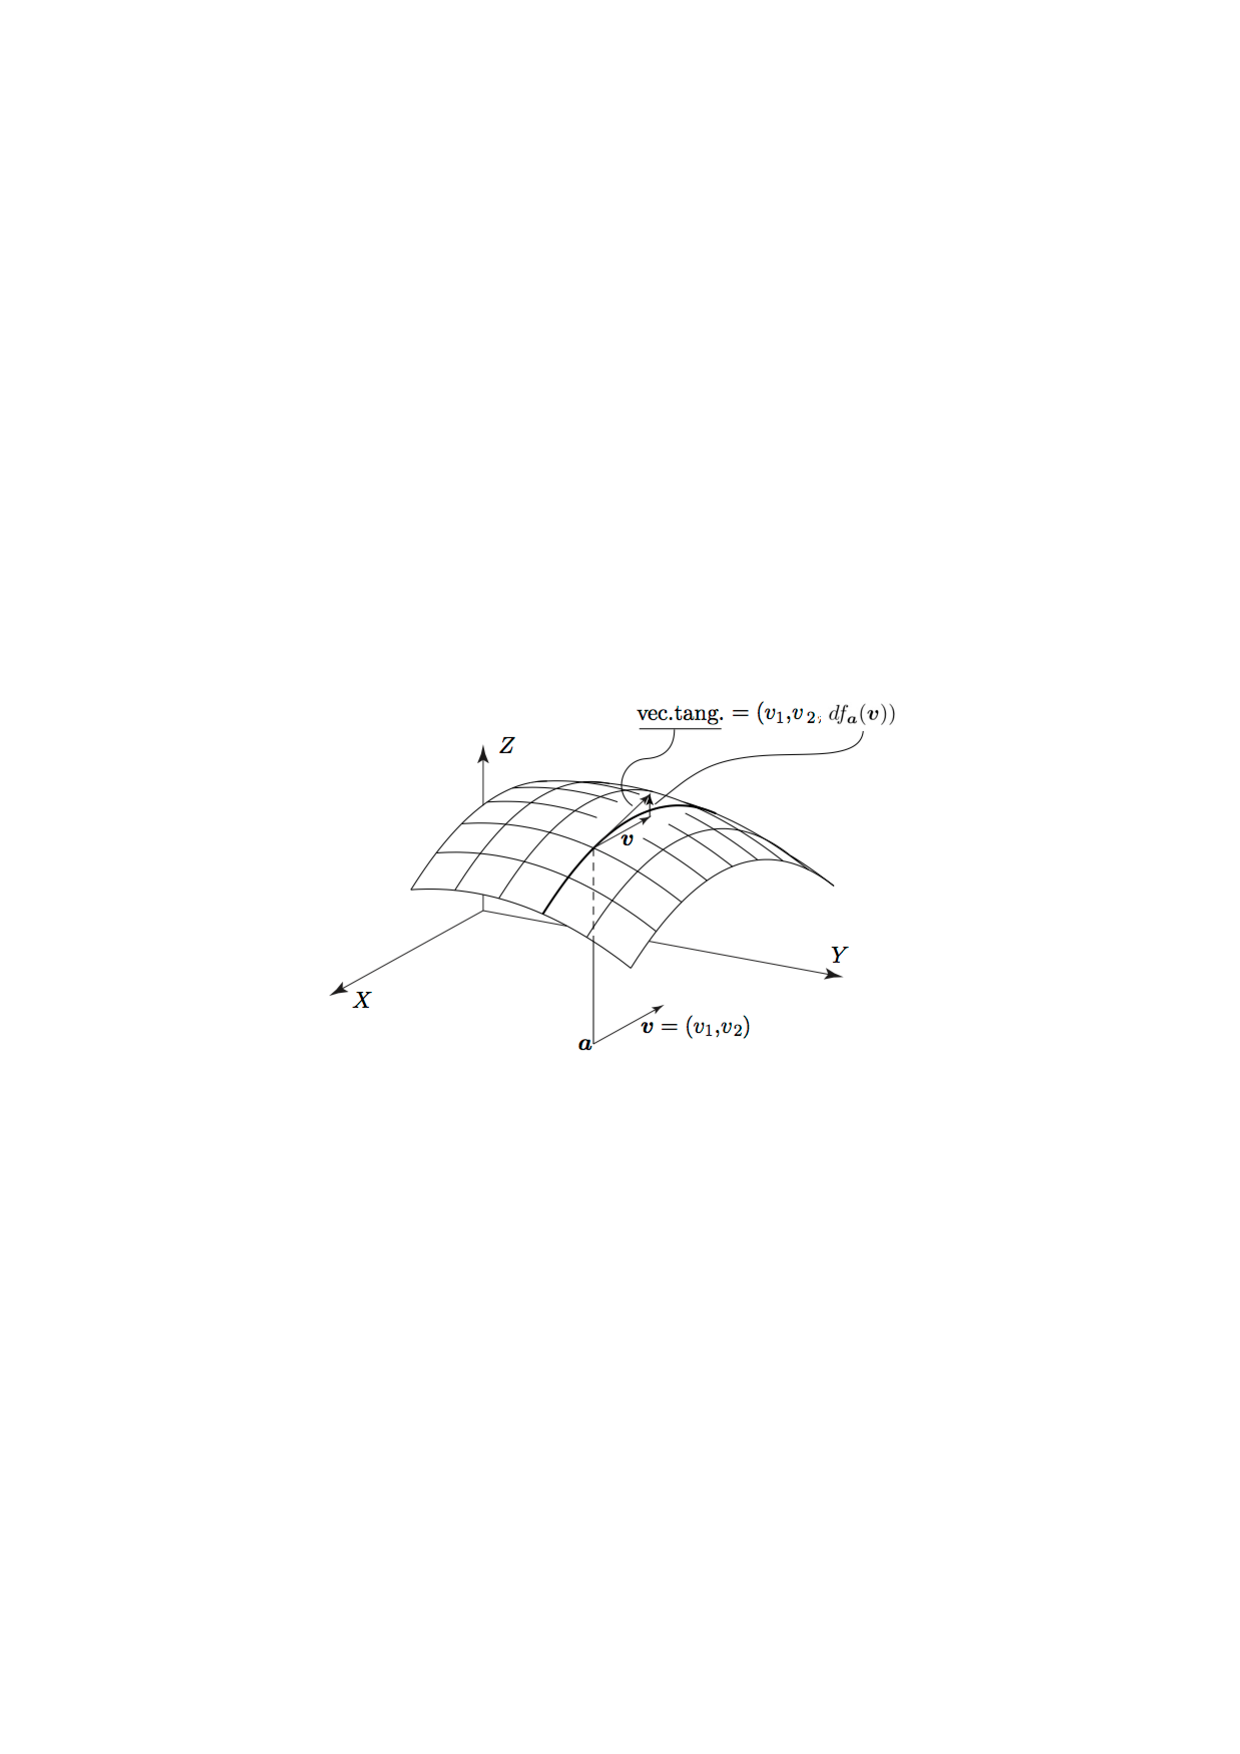
\includegraphics{T2/figs/direccionales.pdf}\\[3cm]
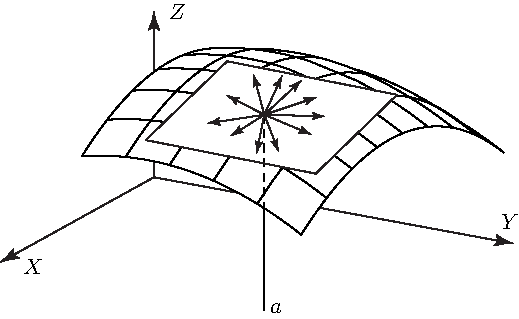
\includegraphics{T2/figs/plano-tangente.pdf}
\end{center}
\caption{Representación de la derivada direccional y vectores tangentes}%
%\caption{Construcción del plano tangente.}\label{fig:pl-tang}
\label{fig:der-dir}
\end{figure}

\begin{ejemplo}
Hemos calculado anteriormente las derivadas parciales del campo 
$f(x,y)=2x^2y-xy^2$:
\begin{align*}
D_1f(x,y)&=\frac{\partial}{\partial x} (2x^2y-xy^2) = 4xy-y^2\\
D_2f(x,y)&=\frac{\partial}{\partial y} (2x^2y-xy^2) = 2x^2-2xy
\end{align*}
Por lo tanto el vector gradiente y la diferencial en el punto $\boldsymbol a=(2,-1)$ son:
\begin{align*}
\nabla f(2,-1)&=(-9,12)\\
df_{(2,-1)}(v_1,v_2)&=\nabla f(2,-1)\cdot(v_1,v_2)=(-9,12)\cdot(v_1,v_2)=
-9v_1+12v_2\tag*{\fej}
\end{align*}
\end{ejemplo}

Ya podemos definir formalmente, \emph{espacio vectorial tangente} y  \emph{espacio afín tangente}.
%
\begin{definicion}\label{def:tang}
Sea $f\colon \mathit{D}\subset \mathbb{R}^n\to \mathbb{R}$ un campo escalar, $\boldsymbol a\in \mathit{D}$.
\begin{enumerate}
\item
El conjunto de los vectores $(v_1,\dots,v_n,v_{n+1})\in\mathbb{R}^{n+1}$ tales que:
\[
D_1f(\boldsymbol a)\cdot v_1 +\dots+D_nf(\boldsymbol a)\cdot v_n-v_{n+1}=0
\]
se denomina \emph{espacio vectorial tangente} al grafo de $f$ en el punto $\boldsymbol a$.
\item
El conjunto de los puntos $(x_1,\dots,x_n,z)\in\mathbb{R}^{n+1}$ tales que:
\[
D_1f(\boldsymbol a)\cdot(x_1-a_1)+\dots+D_nf(\boldsymbol a)\cdot(x_n-a_n)-(z-f(\boldsymbol a))=0
\]
se denomina \emph{espacio (afín) tangente} al grafo de $f$ en el punto $\boldsymbol a$.
Si $n=2$ lo denominamos \emph{plano tangente} y si $n=1$ lo denominamos \emph{recta tangente}.
\end{enumerate}
\end{definicion}

Hemos definido formalemente las nociones de derivada direccional, vector tangente y espacio tangente, y hemos utilizado varias veces la palabra \emph{diferenciabilidad} sin definirla formalmente. 
La existencia de derivadas parciales y de derivadas direccionales, o el hecho de que todos los vectores tangentes formen un plano, no son características necesarias para hablar de diferenciabilidad.
Necesitamos además que \emph{la diferencial del campo sea el campo escalar lineal que mejor lo aproxime en las cercanías del punto~$\boldsymbol a$}.
Está propiedad coincide con la que conocemos para funciones de una variable: \emph{la recta tangente es la que mejor aproxima la función con polinomios de grado 1}.

\begin{definicion}
Sea $f\colon \mathit{D}\subset \mathbb{R}^n\to \mathbb{R}$ un campo escalar y $\boldsymbol a\in \mathit{D}$ para el cual existe el vector gradiente
$\nabla f(\boldsymbol a)$.
Decimos que $f$ es \emph{diferenciable} en $\boldsymbol{a}$ si
\[
\lim_{\boldsymbol{h}\to\boldsymbol{0}}\dfrac{1}{\|\boldsymbol{h}\|}(f(\boldsymbol{a}+\boldsymbol{h})-f(\boldsymbol{a})-\nabla f(\boldsymbol a)\cdot\boldsymbol{h})=0
\]
\end{definicion}

Por lo tanto, el estudio de la propiedad de diferenciabilidad se basa en el cálculo de límites en varias variables que, como ya hemos dicho, no vamos a abordar en este curso.
En la mayoría de los casos, será suficiente con aplicar los resultados que recogemos a continuación y que aseguran la diferenciabilidad de los campos expresados a partir de funciones elementales.
A lo largo del curso, solo vamos a trabajar con este tipo de funciones, y por lo tanto, no será necesario estudiar la condición de diferenciabilidad a partir de la definición.
%
\begin{teorema}
Si existen todas las derivadas parciales del campo escalar $f$ y son continuas en un entorno del punto $\boldsymbol{a}$, entonces $f$ es diferenciable en $\boldsymbol{a}$.
\end{teorema}

La condición dada en este teorema es suficiente para garantizar la diferenciabilidad, pero no es una condición necesaria y, de hecho, se pueden establecer ejemplos bastantes simples de campos diferenciables cuyas derivadas parciales no son continuas.
Si un campo es diferenciable y su parciales son continuas, decimos que el campo es de \emph{clase~$\mathcal C^1$}.

\begin{corolario}
\label{cor:camposc1} Si un campo escalar está determinado por operaciones algebraicas entre funciones elementales
%%
%\footnote{Recordemos que, aunque las funciones potenciales son consideradas
%como elementales, algunos casos suponen una excepción a esta regla; concretamente, si $f(x)=x^\alpha$ y
%$0<\alpha<1$, $f$ no es derivable en 0}
(polinomios, exponenciales, trigonométricas, \dots ),
% en un dominio $\mathit{D}$,
entonces el campo es continuo y diferenciable en el dominio común a todas sus derivadas parciales.
\end{corolario}


\begin{rawhtml}
<p style="text-align: center;"><iframe width="560" height="316" src="https://www.youtube.com/embed/U4LnolPUqdw?list=PL2rtpLKW91qYfkQ_gzsN2-UGxdfRYJ03_" frameborder="0" allowfullscreen=""></iframe></p>
\end{rawhtml}

\begin{rawhtml}
<p style="text-align: center;"><iframe width="560" height="316" src="https://www.youtube.com/embed/CPgUZA-CLl0?list=PL2rtpLKW91qYfkQ_gzsN2-UGxdfRYJ03_" frameborder="0" allowfullscreen=""></iframe></p>
\end{rawhtml}


\subsubsection{Notaciones posibles de derivadas y derivadas parciales}

Hemos utilizado en las páginas anteriores varias notaciones para las derivadas de funciones reales y para las derivadas parciales de campos escalares.
Una de estas notaciones es $D_if(\boldsymbol a)$, que se debe a Louis François Antoine Arbogast y extiende la notación $Df(a)$ para la derivada de funciones reales,
aunque para funciones de una variable, la notación más utilizada es $f'(a)$, que se debe a Joseph-Louis Lagrange.
Estas notaciones son adecuadas para aplicarlas sobre el nombre de la función.
Sin embargo, en muchas ocasiones trabajamos sobre campos sin utilizar un nombre específico, en estos casos, debemos utilizar la \emph{notación de Leibniz}, que toma su nombre de Gottfried Wilhelm Leibniz,
\[
\dfrac{d}{dx}f(x)\hspace{.2\textwidth} \dfrac{\partial}{\partial x_i}f(x_1,\dots,x_n)
\]

\subsubsection{Propiedades del vector gradiente}

%Hemos utilizado en las páginas anteriores varias notaciones para las derivadas de funciones reales y para las derivadas parciales de campos escalares.
%Una de estas notaciones es $D_if(\boldsymbol a)$, que se debe a Louis François Antoine Arbogast y extiende la notación $Df(a)$ para la derivada de funciones reales;
%aunque para funciones de una variable, la notación más utilizada es $f'(a)$, que se debe a Joseph-Louis Lagrange.
%Estas notaciones son adecuadas para aplicarlas sobre el nombre de la función; sin embargo, en muchas ocasiones trabajamos sobre campos sin utilizar un nombre específico, en estos casos, debemos utilizar las \emph{notaciones de Leibniz}, que se debe a Gottfried Wilhelm Leibniz,
%\[
%\dfrac{d}{dx}f(x),\hspace{.2\textwidth} \dfrac{\partial}{\partial x_i}f(x_1,\dots,x_n)
%\]

La siguiente proposición establece que la relación entre continuidad y derivabilidad de las funciones reales se mantiene en la generalización a campos.
%
\begin{proposicion} Si $f$ es un campo escalar diferenciable en $\boldsymbol{a}$, entonces $f$ es continuo en $\boldsymbol{a}$.
\end{proposicion}
%
Aunque en el estudio de campos concretos, no necesitaremos normalmente la aplicación de las propiedades algebraicas que vemos a continuación, estas pueden ser útiles en algunas situaciones para simplificar cálculos y realizar desarrollos teóricos simples.

\begin{proposicion}\label{prop-alg} Consideremos los campos $f\colon\mathbb{R}^n\to\mathbb{R}$, $g\colon\mathbb{R}^n\to\mathbb{R}$, la función real $\phi\colon\mathbb{R}\to\mathbb{R}$ y la función vectorial $\boldsymbol\gamma\colon\mathbb{R}\to\mathbb{R}^n$.
\begin{enumerate}
\item
Si $f$ y $g$ son diferenciables en $\boldsymbol{a}$, entonces $f+g$ es diferenciable en $\boldsymbol{a}$ y
\[
\nabla(f+g)(\boldsymbol{a})=\nabla f(\boldsymbol{a})+\nabla g(\boldsymbol{a})
\]
\item
Si $f$ y $g$ son diferenciables en $\boldsymbol{a}$, entonces $fg$ también es diferenciable en $\boldsymbol{a}$ y
\[
\nabla(fg)(\boldsymbol{a})=g(\boldsymbol{a})\nabla f(\boldsymbol{a})+f(\boldsymbol{a})\nabla g(\boldsymbol{a})
\]
\item Si $f$ es diferenciable en $\boldsymbol{a}$ y $f(\boldsymbol{a})\neq 0$, entonces $1/f$ es diferenciable en $\boldsymbol{a}$ y
\[
\nabla(1/f)(\boldsymbol{a})=\frac{-1}{[f(\boldsymbol{a})]^2}\nabla f(\boldsymbol{a})
\]
\item
Regla de la cadena: Si $f$ es diferenciable en $\boldsymbol{a}$ y $\phi$ es derivable en $f(\boldsymbol{a})$, entonces $\phi\circ f$ es diferenciable en $\boldsymbol{a}$ y 
\[
\nabla(\phi\circ f)(\boldsymbol a)=\phi'(f(\boldsymbol{a}))\nabla f(\boldsymbol a)
\]
\item
Regla de la cadena: Si $\boldsymbol\gamma$ es derivable en $t_0$ y $f$ es diferenciable en $\boldsymbol\gamma(t_0)$, entonces $f\circ \boldsymbol\gamma$ es derivable en $t_0$ y 
\[
(f\circ \boldsymbol\gamma)'(t_0)=\nabla f(\boldsymbol\gamma(t_0))\cdot
\boldsymbol\gamma'(t_0)
\]
\end{enumerate}
\end{proposicion}
%
Deducimos a continuación una importante propiedad del vector gradiente.
Si $\boldsymbol{u}$ es un vector unitario,
según hemos definido anteriormente, la derivada direccional de un campo $f$ en un punto $\boldsymbol a$ y en la dirección $\boldsymbol u$ es:
\[
D_{\boldsymbol{u}}f(\boldsymbol{a})= \nabla f(\boldsymbol{a})\cdot\boldsymbol{u}
=\|\nabla f(\boldsymbol{a})\|\cos\alpha
\]
en donde $\alpha$ es el ángulo formado por los vectores $\boldsymbol{u}$ y $\nabla f(\boldsymbol{a})$.
Por lo tanto, dado que el módulo del vector gradiente es constante, el valor de la derivada direccional depende solamente del ángulo que el vector gradiente forma con la dirección considerada.
%
\begin{teorema}\label{th:gradiente}
Sea $\alpha$ es ángulo formado por $\nabla f(\boldsymbol a)$ y un vector unitario $\boldsymbol u$.
\begin{enumerate}
\item\label{th:grad-par}
Si $\alpha=0$ (los vectores $\boldsymbol u$ y $\nabla f(\boldsymbol a)$ tienen la misma dirección), el valor del coseno es máximo y por lo tanto, el valor de la derivada direccional es máximo e igual a
$D_{\boldsymbol u}f(a)=\|\nabla f(\boldsymbol{a})\|$.
\item\label{th:grad-perp}
Si $\alpha=\pi/2$ (los vectores $\boldsymbol u$ y $\nabla f(\boldsymbol a)$ son perpendiculares) el valor del coseno es 0, es decir, derivada direccional es nula en la dirección perpendicular al vector gradiente.
\end{enumerate}
\end{teorema}
%
\begin{figure}
\begin{center}
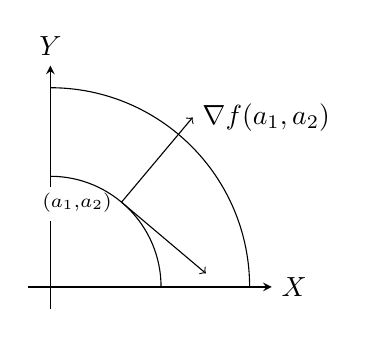
\begin{tikzpicture}[x=4em,y=4em]
\draw[-stealth] (-.2,0) -- (2,0) node[right] {$X$}; 
\draw (0,-.2) -- (0,.6);
\draw[-stealth] (0,.9) -- (0,2) node[above] {$Y$};
\draw (0,0) +(0:1) arc (0:90:1);
\draw (0,0) +(0:1.8) arc (0:90:1.8);
\draw[->] (0,0) +(50:1) -- +(50:2) node[right]
{$\nabla f(a_1,a_2)$};
\draw (0,0) +(50:1) node[left] {$\scriptstyle(a_1,a_2)$};
\draw[->] (0,0) +(50:1) --(5:1.41);
\end{tikzpicture}
\end{center}
\caption{El gradiente da la dirección de derivada direccional máxima.}\label{fig:grad-max}
\end{figure}
%
En la figura~\ref{fig:grad-max} representamos dos curvas de nivel de un campo $f$. Si nos movemos desde el punto $(a_1,a_2)$ y queremos sufrir el cambio más rápido en el valor del campo, tendremos que ir en la dirección que nos da mayor proximidad a la siguiente curva de nivel.
El ítem~\ref{th:grad-par} del teorema~\ref{th:gradiente} indica que esta dirección es la dada por el vector gradiente de $f$ en ese punto.

Pero si nos movemos sobre la curva de nivel, no sufrimos ninguna variación en el valor del campo, es decir, la derivada direccional es 0;
el ítem~\ref{th:grad-perp} del teorema~\ref{th:gradiente}
dice que esta dirección es normal al vector gradiente.
Esta propiedad es válida para cualquier campo, como probamos a continuación.

Sea $\boldsymbol\gamma\colon I\subset\mathbb{R}\to\mathbb{R}^n$ la parametrización de una curva contenida en una superficie de nivel de un campo $f$, es decir, $f(\boldsymbol\gamma(t))=c$ para todo $t$, y supongamos que esta curva pasa por el punto $\boldsymbol a$, es decir, $\boldsymbol\gamma(t_0)=\boldsymbol a$.
Una simple aplicación de la regla de la cadena justifica el siguiente desarrollo:
\[
0=(f\circ \boldsymbol\gamma)'(t_0)=
\nabla f(\boldsymbol\gamma(t_0))\cdot\boldsymbol\gamma'(t_0)
\]
El vector derivada $\boldsymbol\gamma'(t_0)$ es tangente a la curva y por lo tanto a la superficie de nivel; en consecuencia, la igualdad anterior permite afirmar que estos vectores son perpendiculares al vector gradiente (ver figura~\ref{fig:sup-niv}).
%
\begin{teorema}\label{teo:tang-nivel}
Sea $f\colon \mathit{D}\subset\mathbb{R}^n\to \mathbb{R}$ un campo diferenciable y consideremos una superficie de nivel $f(\boldsymbol x)=c$ y un punto $\boldsymbol a$ en dicha superficie.
Entonces, $\nabla f(\boldsymbol a)$ es un vector normal al plano tangente a la superficie de nivel en punto~$\boldsymbol a$.
Por lo tanto, el espacio vectorial tangente a la superficie es:
\[
\nabla f(\boldsymbol a)\cdot\boldsymbol v =0
\]
y el espacio afín tangente es:
\[
\nabla f(\boldsymbol a)\cdot(\boldsymbol x -\boldsymbol a)=0
\]
\end{teorema}
%
Como casos particulares, vamos a mostrar las expresiones de las rectas y planos tangentes a curvas de nivel en $\mathbb{R}^2$ y superficies de nivel en $\mathbb{R}^3$:
%
\begin{figure}
\begin{center}
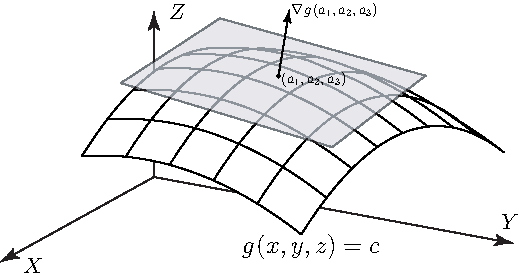
\includegraphics{T2/figs/grad-sup-nivel.pdf}
\end{center}
\caption{El gradiente es normal a la superficie de nivel.}
\label{fig:sup-niv}
\end{figure}
%
\begin{enumerate}
\item
La recta tangente a la curva dada por $f(x,y)=c$ en un punto~$(x_0,y_0)$~es:
\[
D_1f(x_0,y_0)(x-x_0)+D_2f(x_0,y_0)(y-y_0)=0
\]
\item
Análogamente, el plano tangente a la superficie dada por $g(x,y,z)=c$ (ver figura~\ref{fig:sup-niv}) en un punto $(x_0,y_0,z_0)$ es:
\[
D_1g(x_0,y_0,z_0)(x-x_0)+D_2g(x_0,y_0,z_0)(y-y_0)+D_3g(x_0,y_0,z_0)(z-z_0)=0
\]
\end{enumerate}

\begin{rawhtml}
<p style="text-align: center;"><iframe width="560" height="316" src="https://www.youtube.com/embed/Yh3GFRJ8_ng?list=PL2rtpLKW91qYfkQ_gzsN2-UGxdfRYJ03_" frameborder="0" allowfullscreen=""></iframe></p>
\end{rawhtml}

\begin{ejemplo}
En la lección anterior, hemos aprendido a calcular las rectas tangentes a curvas parametrizadas.
En particular, podríamos obtener la recta tangente a una cónica utilizando las parametrizaciones que hemos introducido para las cónicas.
Ahora, haciendo uso del vector gradiente, podemos calcular más fácilmente estas rectas.
Por ejemplo, la elipse
\[
\dfrac{x^2}{a^2}+\dfrac{y^2}{b^2}=1
\]
es una curva de nivel del campo
\[
f(x,y)=\dfrac{x^2}{a^2}+\dfrac{y^2}{b^2}
\]
y por lo tanto, un vector normal a dicha curva en un punto $(x_0,y_0)$ es
\[
\nabla f(x,y)=\left(\dfrac{2x_0}{a^2},\dfrac{2y_0}{b^2}\right)
\]
En consecuencia, la recta tangente es:
\begin{align*}
\dfrac{2x_0}{a^2}(x-x_0)+\dfrac{2y_0}{b^2}(y-y_0)&=0\\
\dfrac{x_0}{a^2}(x-x_0)+\dfrac{y_0}{b^2}(y-y_0)&=0\\
\dfrac{x_0}{a^2}x-\dfrac{x_0^2}{a^2}+\dfrac{y_0}{b^2}y-\dfrac{y_0^2}{b^2}&=0\\
\dfrac{x_0}{a^2}x+\dfrac{y_0}{b^2}y&=\dfrac{x_0^2}{a^2}+\dfrac{y_0^2}{b^2}\\
\dfrac{x_0}{a^2}x+\dfrac{y_0}{b^2}y&=1\tag*{\fej}
\end{align*}
\begin{rawhtml}
<p style="text-align: center;"><iframe width="560" height="316" src="https://www.youtube.com/embed/JM15VqSUl04?list=PL2rtpLKW91qYfkQ_gzsN2-UGxdfRYJ03_" frameborder="0" allowfullscreen=""></iframe></p>
\end{rawhtml}
\end{ejemplo}
%
\begin{ejemplo}
Dado un campo escalar en $\mathbb{R}^2$, su grafo puede considerarse como la superficie de nivel de un campo en $\mathbb{R}^3$:
\[
g(x,y,z)=f(x,y)-z.
\]
Efectivamente, si $g(x,y,z)=0$, entonces $z=f(x,y)$.
Por lo tanto, el plano tangente a $g(x,y,z)=0$ es normal al vector
\[
\nabla g(x_0,y_0,z_0)=(D_1f(x_0,y_0),D_2f(x_0,y_0),-1),
\]
que permite construir el plano tangente introducido en la definición~\ref{def:tang}:
\[
D_1f(x_0,y_0)(x-x_0)+D_2f(x_0,y_0)(y-y_0)-(z-f(x_0,y_0))=0\tag*{\fej}
\]
\end{ejemplo}


\subsection{Derivadas de orden superior}

Para un campo $f\colon \mathit{D}\subset\mathbb{R}^n\to\mathbb{R}$ diferenciable hemos definido las derivadas parciales
para cada punto del dominio y por lo tanto, estas definen un campo escalar para cada $i$ con $1\leq i\leq n$:
\[
D_i f\colon \mathit{D}\subset\mathbb{R}^n\to \mathbb{R}
\]
Tiene entonces sentido estudiar la diferenciabilidad de estos campos y calcular sus derivadas parciales.
Las derivadas parciales de los campos $D_if$ se denominan \emph{derivadas de segundo orden} de $f$ y las notaciones posibles para ellas son
\[
\frac{\partial}{\partial x_i}\left(\frac{\partial f}{\partial x_j}\right)=
\dfrac{\partial^2 f}{\partial x_i\partial x_j},\qquad\qquad
D_i(D_jf)=D_{i j}f.
\]
Por el corolario~\ref{cor:camposc1}, la continuidad de las derivadas parciales de segundo orden asegura la diferenciabilidad de las derivadas parciales de $f$;
en tal caso, decimos que $f$ es de
\emph{clase $\mathcal C^2$}.
Una importante propiedad de estos campos queda establecida por el siguiente teorema, que asegura que el orden de derivación no influye en el resultado.
%
\begin{teorema}[de Schwarz]
Sea $f$ un campo escalar tal que sus derivadas parciales de segundo orden son continuas; entonces,
para cada $i$, $j$:
\[
D_{ij}f=D_{ji}f
\]
\end{teorema}
%
Para los campos de clase $\mathcal C^2$ y para cada punto de su dominio, definimos la siguiente matriz $n\times n$, que se denomina \emph{matriz Hessiana} de $f$ en $\boldsymbol a$:
\[
\nabla^2f(\boldsymbol{a}) =
\left(\begin{array}{cccc}
D_{11}f(\boldsymbol{a}) & D_{12}f(\boldsymbol{a}) & \cdots & D_{1n}f(\boldsymbol{a})\\
D_{21}f(\boldsymbol{a}) & D_{22}f(\boldsymbol{a}) & \cdots & D_{2n}f(\boldsymbol{a})\\
\cdots & \cdots & \ddots & \cdots\\
D_{n1}f(\boldsymbol{a}) & D_{n2}f(\boldsymbol{a}) & \cdots & D_{nn}f(\boldsymbol{a})
\end{array}\right)
\]
Obsérvese que, por el teorema de Schwarz, esta matriz es simétrica.
A partir de ella, definimos el campo
\[
d^2f_{\boldsymbol a}(\boldsymbol{u})=\boldsymbol{u}^t\nabla^2f(\boldsymbol{a})\boldsymbol{u},
\]
que se denomina \emph{segunda diferencial de $f$ en $\boldsymbol a$}.
Como ya dijimos anteriormente, cuando trabajamos con expresiones matriciales, los vectores deben tratarse como matrices columna y por esta razón escribimos la matriz transpuesta $\boldsymbol{u}^t$ a la izquierda de la matriz hessiana.
%
\begin{ejemplo}
Vamos a calcular $d^2f_{\boldsymbol a}$ para $f(x,y)=2x^2y-xy^2$ y $\boldsymbol a=(2,-1)$:
\begin{align*}
f(x,y) &= 2x^2y-xy^2 \\
\nabla f(x,y) &= (4xy-y^2,2x^2-2xy) \\
\nabla^2 f(x,y) &=
\begin{pmatrix}
4y & 4x-2y \\
4x-2y & -2x
\end{pmatrix}\\
\nabla^2 f(2,-1) &=
\begin{pmatrix}
-4 & 10 \\
10 & -4
\end{pmatrix}\\
d^2f_{(2,-1)}(u_1,u_2)&=(u_1\ u_2)
\begin{pmatrix}
-4 & 10 \\
10 & -4
\end{pmatrix}\begin{pmatrix}
u_1 \\
u_2
\end{pmatrix}\\
d^2f_{(2,-1)}(u_1,u_2)&=-4u_1^2+20u_1u_2-4u_2^2\tag*{\fej}
\end{align*}
\end{ejemplo}
Como vemos en este ejemplo, la expresión obtenida para $d^2f_{(2,-1)}$ es un polinomio de grado 2 sin términos de grado 1 o grado 0; estas expresiones se denominan \emph{formas cuadráticas}.

\begin{rawhtml}
<p style="text-align: center;"><iframe width="560" height="316" src="https://www.youtube.com/embed/26HHBREHqO8?list=PL2rtpLKW91qYfkQ_gzsN2-UGxdfRYJ03_" frameborder="0" allowfullscreen=""></iframe></p>
\end{rawhtml}

Todo el desarrollo mostrado en esta sección puede continuarse para definir las derivadas parciales de órdenes superiores (orden tres, cuatro,\dots).
Sin embargo, en este curso solo trabajaremos con las derivadas de segundo orden.
Por ejemplo, con estas derivadas, podemos mejorar la aproximación dada por el vector gradiente en la definición de diferenciabilidad.
%
\begin{teorema}[Fórmula de Taylor]
Sea $f\colon \mathit{D}\subset\mathbb{R}^n\to\mathbb{R}$
un campo escalar dos veces diferenciable y con parciales de segundo orden continuas.
Entonces:
\[
f(\boldsymbol{a}+\boldsymbol{u})=
f(\boldsymbol{a})+\nabla f(\boldsymbol{a})\cdot\boldsymbol{u}
+\frac{1}{2}\boldsymbol{u}^t\nabla^2f(\boldsymbol{a})\boldsymbol{u}+
\|\boldsymbol{u}\|^2E(\boldsymbol{a},\boldsymbol{u}),
\]
en donde $\displaystyle\lim_{\|\boldsymbol{u}\|\to 0}E(\boldsymbol{a},\boldsymbol{u})=0$.
\end{teorema}
%
Es decir, el campo $f(\boldsymbol{a}+\boldsymbol{u})$, en un entorno lo suficientemente pequeño de $\boldsymbol a$, tiene un comportamiento ``parecido'' al polinomio de segundo orden
\[
f(\boldsymbol{a})+\nabla f(\boldsymbol{a})\cdot\boldsymbol{u}
+\frac{1}{2}\boldsymbol{u}^t\nabla^2f(\boldsymbol{a})\boldsymbol{u}.
\]
Este polinomio también lo podemos escribir como:
\[
T(\boldsymbol x)=f(\boldsymbol{a})+\nabla f(\boldsymbol{a})\cdot(\boldsymbol x-\boldsymbol a)
+\frac{1}{2}(\boldsymbol x-\boldsymbol a)^t\nabla^2f(\boldsymbol{a})(\boldsymbol x-\boldsymbol a).
\]
%
\begin{ejemplo}
%En el ejemplo~\ref{ej:aprox} determinamos una aproximación del campo $f(x,y)=\operatorname{sen}(x^2+y)$ en $x=0.1$, $y=0.1$ usando el gradiente en $(0,0)$.
%Vamos a mejorar esta aproximación utilizando el polinomio de Taylor de orden 2.
Vamos a calcular el polinomio de Taylor de
$f(x,y)=\operatorname{sen}(x^2+y)$ de orden 2 en el punto $(0,0)$:
%
\begin{align*}
\nabla f(x,y)&= (2x\cos(x^2+y),\cos(x^2+y))\\
\nabla f(0,0)&= (0,1)\\
\nabla^2 f(x,y)&=
\begin{pmatrix}
2\cos(x^2+y)-4x^2\operatorname{sen}(x^2+y) & -2x\operatorname{sen}(x^2+y)\\
-2x\operatorname{sen}(x^2+y) & -\operatorname{sen}(x^2+y)
\end{pmatrix}\\
\nabla^2 f(0,0)&=
\begin{pmatrix}
2 & 0 \\
0 & 0
\end{pmatrix}\\
f(x,y)\approx  T(x,y) & =0+(0,1)\cdot(x,y)+\frac12(x\ y)
\begin{pmatrix}
2 & 0 \\
0 & 0
\end{pmatrix}
\begin{pmatrix}
x \\
y
\end{pmatrix}
=y+x^2\tag*{\fej}
%\\
%f(0.1,0.1)&\approx 0.1+0.01=0.11\\
%f(0.1,0.1)&=\operatorname{sen}(0.11)=0.1097\dots
\end{align*}
%Como se observa, el resultado obtenido ahora está más cerca del valor real que el obtenido
%en el ejemplo~\ref{ej:aprox}.\fej
\end{ejemplo}

\begin{rawhtml}
<p style="text-align: center;"><iframe width="560" height="316" src="https://www.youtube.com/embed/uyhSppC0mFU?list=PL2rtpLKW91qYfkQ_gzsN2-UGxdfRYJ03_" frameborder="0" allowfullscreen=""></iframe></p>
\end{rawhtml}

\newpage

%\thispagestyle{empty}
%\ 
%
%\vfill
%\begin{center}
%(Esta página se ha dejado intencionalmente en blanco)
%\end{center}
%\newpage

\section{Optimización de campos escalares}

Una de las aplicaciones del concepto de diferenciabilidad es resolver problemas de \emph{optimización}, es decir, encontrar los valores máximos y mínimos de una magnitud definida a partir de uno o varios parámetros.
Estos problemas se resuelven fácilmente si la magnitud solo depende de un parámetro, utilizando las derivadas de orden superior de la función de una variable determinada por el problema.
El objetivo de esta lección es generalizar esta técnica a campos escalares, es decir, optimizar magnitudes escalares que dependen de varios parámetros.

Empezamos introducción algunos conceptos y resultados básicos.
%A lo largo de la lección, 
%
%Empezamos introduciendo formalmente la noción de
%\emph{entorno} en $\mathbb{R}^n$.
%%
%\begin{definicion}\label{def:entorno}
%Llamamos \emph{bola abierta de radio $\varepsilon$ y centro $\boldsymbol a\in\mathbb{R}^n$} al conjunto
%\[
%B(\boldsymbol a,\varepsilon)=\{\boldsymbol x\in\mathbb{R}^n\mid \|\boldsymbol x-\boldsymbol a\|<\varepsilon\}.
%\]
%Decimos que un conjunto $E$ es un \emph{entorno} del punto $\boldsymbol a$, si existe $\varepsilon>0$ tal que
%$B(\boldsymbol a,\varepsilon)\subset E$.
%\end{definicion}
%%
%En particular, para $n=2$, las bolas abiertas son círculos de radio $\varepsilon$ y centro en $\boldsymbol a$:
%\begin{multline*}
%B((a_1,a_2),\varepsilon)=
%\{(x,y)\mid \sqrt{(x-a_1)^2+(y-a_2)^2}<\varepsilon\}=\\
%=\{(x,y)\mid (x-a_1)^2+(y-a_2)^2<\varepsilon^2\}.
%\end{multline*}
%Análogamente, para $n=3$, las bolas abiertas son esferas de radio $\varepsilon$ y centro en $\boldsymbol a$:
%\[
%B((a_1,a_2,a_3),\varepsilon)=
%\{(x,y,z)\mid (x-a_1)^2+(y-a_2)^2+(z-a_3)^2<\varepsilon^2\}.
%\]
%
%Utilizaremos la noción de entorno para definir diversos conceptos, como conjunto acotado, conjunto cerrado y extremo local.

\begin{definicion}
Un conjunto $\mathit{D}\subset \mathbb{R}^n$ se dice que está \emph{acotado} si existe $r>0$
tal que $\|\boldsymbol{x}-\boldsymbol{y}\|\sle r$ para todo $\boldsymbol x,\boldsymbol y\in D$.
\end{definicion}

Es decir, un conjunto está acotado si la distancia entre cualquier par de puntos ($\|\boldsymbol{x}-\boldsymbol{y}\|$) es siempre menor que una cota fija ($\|\boldsymbol{x}-\boldsymbol{y}\|\sle r$).

\begin{definicion}
Un conjunto $\mathit{D}\subset \mathbb{R}^n$ se dice que es \emph{cerrado}
si para todo $\boldsymbol x\not\in D$ existe $r>0$ tal que:
si $\|\boldsymbol{x}-\boldsymbol{y}\|\sle r$, entonces $\boldsymbol y\not\in D$.
\end{definicion}

Es decir, un conjunto es cerrado si cualquier punto que no pertenezca a él esta ``separado'' del conjunto, es decir, la distancia a cualquier punto del conjunto es estrictamente positiva.

Sabemos que una función de una variable, continua en un dominio cerrado y acotado siempre alcanza un valor máximo y un valor mínimo en tal dominio.
Esta propiedad también se verifica para campos escalares.
%
\begin{teorema} Sea $f$ un campo escalar continuo en un conjunto $\mathit{D}$ cerrado y acotado.
Entonces existen $\boldsymbol{x}_0,\boldsymbol{x}_1\in\mathit{D}$ tales que $f(\boldsymbol{x}_0)\leq f(\boldsymbol x)\leq f(\boldsymbol{x}_1)$ para todo $\boldsymbol{x}\in\mathit{D}$.
\end{teorema}
%
Es decir, $f(\boldsymbol{x}_0)$ es el valor mínimo que toma el campo en el conjunto $\mathit{D}$ y $f(\boldsymbol{x}_1)$ es el valor máximo. En tal caso, decimos que $\boldsymbol{x}_0$ es un punto mínimo y $\boldsymbol{x}_1$ es un punto máximo.

\begin{rawhtml}
<p style="text-align: center;"><iframe width="560" height="316  " src="https://www.youtube.com/embed/OetxytqtDy4?list=PL2rtpLKW91qYfkQ_gzsN2-UGxdfRYJ03_" frameborder="0" allowfullscreen=""></iframe></p>
\end{rawhtml}

\subsection{Extremos locales}

Igual que en el caso real, para determinar los máximos y mínimos de un campo debemos empezar por determinar los máximos y mínimos locales o relativos, es decir, los máximos y mínimos respecto de los puntos cercanos~a~él.

\begin{definicion-br}
\begin{enumerate}
\item
$f\colon \mathit{D}\subset\mathbb{R}^n\to\mathbb{R}$ tiene un
\emph{máximo local (o relativo)} en $\boldsymbol{a}\in \mathit{D}$ si existe $r>0$, tal que $f(\boldsymbol{a})\geq f(\boldsymbol{x})$ para todo $\boldsymbol{x}\in D$ tal que $\|\boldsymbol x-\boldsymbol{a}\|\sle r$.
\item
$f\colon \mathit{D}\subset\mathbb{R}^n\to\mathbb{R}$ tiene un
\emph{mínimo local (o relativo)} en $\boldsymbol{a}\in \mathit{D}$ si existe
$r>0$, tal que $f(\boldsymbol{a})\leq f(\boldsymbol{x})$ para todo $\boldsymbol{x}\in D$ tal que $\|\boldsymbol x-\boldsymbol{a}\|\sle r$.
\end{enumerate}
\end{definicion-br}
%
Utilizaremos la denominación genérica de \emph{extremo} local para referirnos a un punto que sea máximo local o mínimo local.
El siguiente teorema justifica la definición de puntos críticos, entre los cuales encontramos los extremos locales de un campo.
%
\begin{teorema}\label{teo:crit}
Si $f\colon \mathit{D}\subset\mathbb{R}^n\to\mathbb{R}$ es un campo escalar diferenciable y $\boldsymbol{a}\in \mathit{D}$ es un extremo local de $f$, entonces $\nabla f(\boldsymbol a)=\boldsymbol 0=(0,\dots,0)$;
es decir, todas las derivadas parciales de $f$ en  $\boldsymbol{a}$ son nulas.
\end{teorema}
%
Gráficamente, para funciones de una variable sabemos que la recta tangente al grafo de la función en un extremo son paralelas al eje $OX$.
Si $n=2$ también obtenemos una propiedad parecida, ya que si $\nabla f(a_1,a_2)=(0,0)$, entonces el plano tangente al grafo en el punto $(a_1,a_2)$ es perpendicular al vector $(0,0,-1)$, es decir, es paralelo al plano $XY$.
%
\begin{ejemplo-br}\label{ej:x2-y2}
\begin{enumerate}
\item
Para el campo $f(x,y)=x^2+y^2$ se verifica que $\nabla f(x,y)=(2x,2y)$ y por lo tanto, su único punto crítico es $(x_0,y_0)=(0,0)$.
Es fácil razonar que este punto es mínimo del campo:
\[
x^2+y^2 \geq 0 =f(0,0)
\]
\item
Para el campo $f(x,y)=x^2-y^2$ se verifica que $\nabla f(x,y)=(2x,-2y)$ y por lo tanto, su único punto crítico es $(x_0,y_0)=(0,0)$.
En este caso, el punto no es un extremo ya que $f(0,0)=0$, $f(x,0)=x^2>0$ para todo $x\ne 0$, $f(0,y)=-y^2\sle 0$ para todo $y\ne 0$.\fej
\end{enumerate}
\end{ejemplo-br}
%
Los puntos en los cuales el vector gradiente es nulo se denominan \emph{puntos críticos}.
En el ejemplo anterior, hemos visto que no todos los puntos críticos son máximos o mínimos; los puntos críticos que no son extremos locales se denominan \emph{puntos silla}.

\begin{rawhtml}
<p style="text-align: center;"><iframe width="560" height="316" src="https://www.youtube.com/embed/gPs8SrICbAg?list=PL2rtpLKW91qYfkQ_gzsN2-UGxdfRYJ03_" frameborder="0" allowfullscreen=""></iframe></p>
\end{rawhtml}

Por lo tanto, para determinar los extremos locales de un
campo escalar diferenciable,  debemos localizar los puntos críticos y estudiar cuáles son máximos, cuáles mínimos y cuáles no son extremos.
Esta clasificación puede hacerse comparando directamente el valor del campo en esos puntos con el valor en los puntos ``cercanos'' a él, como hemos hecho en el ejemplo anterior, aunque en muchos casos será preferible utilizar los métodos que vemos a continuación.

\newpage
\begin{ejemplo}
Los puntos críticos del campo $f(x,y)=xy^2e^{xy}$ son los puntos de la forma $(a,0)$ para todo $a\in\mathbb{R}$, como vemos a continuación.
\begin{align*}
D_1f(x,y)&=y^2(1+xy)e^{xy} = 0 \\
D_2f(x,y)&=xy(2+xy)e^{xy} = 0
\end{align*}
Por lo tanto, efectivamente si $y=0$ se verifican las dos ecuaciones. 
Si $y$ no es igual a $0$, por la segunda ecuación $x$ sería igual a $0$ y en tal caso no se verificaría la primera ecuación.

Vamos a clasificar estos puntos críticos.
\begin{itemize}
\item
Si $a>0$, entonces el punto $(a,0)$ es mínimo: dado que $a$ es estrictamente positivo, los valores de $x$ cercanos a $a$ son también positivos y entonces 
\[
f(x,y)=xy^2e^{xy}\stackrel{(+++)}{>}0=f(a,0)
\]
\item
Si $a\sle 0$, entonces el punto $(a,0)$ es máximo: dado que $a$ es estrictamente negativo, los valores de $x$ cercanos a $a$ son también negativos y entonces 
\[
f(x,y)=xy^2e^{xy}\stackrel{(-++)}{\sle }0=f(a,0)
\]
\item
Finalmente, el punto $(0,0)$ es un punto silla: si tomamos valores de $x$ cercanos a $0$ pero positivos, entonces $f(x,y)=xy^2e^{xy}\ge 0 = f(0,0)$;
si tomamos valores de $x$ cercanos a $0$ pero negativos, entonces $f(x,y)=xy^2e^{xy}\le 0 = f(0,0)$.\hfill$\Box$
\end{itemize}
\end{ejemplo}

\paragraph{Criterio de la hessiana.}
En los ejemplos que hemos visto hasta ahora, hemos podido clasificar fácilmente los puntos críticos comparando el valor de la función en ese punto con el valor en los puntos cercanos a él.
Sin embargo, esto no será siempre posible o fácil de hacer.
En general, la forma más sencilla de hacer la clasificación de los puntos críticos es utilizando, si es posible, el polinomio de Taylor que vimos en la lección anterior.
Recordemos que el teorema de Taylor dice que, en un entorno suficientemente pequeño de $\boldsymbol a$
\[
f(\boldsymbol x) \approx
f(\boldsymbol{a})+\nabla f(\boldsymbol{a})\cdot(\boldsymbol x-\boldsymbol a)
+\frac{1}{2}(\boldsymbol x-\boldsymbol a)^t\nabla^2f(\boldsymbol{a})(\boldsymbol x-\boldsymbol a)
\]
Si, además, $\boldsymbol a$ es un punto crítico, entonces
\begin{align*}
f(\boldsymbol x) &\approx
f(\boldsymbol{a})+\frac{1}{2}(\boldsymbol x-\boldsymbol a)^t\nabla^2f(\boldsymbol{a})
(\boldsymbol x-\boldsymbol a)\\
f(\boldsymbol x) - f(\boldsymbol{a})
&\approx\frac{1}{2}(\boldsymbol x-\boldsymbol a)^t\nabla^2f(\boldsymbol{a})
(\boldsymbol x-\boldsymbol a)\\
\end{align*}
Y en consecuencia, la comparación de $f(\boldsymbol a)$ y $f(\boldsymbol x)$ se reduce a analizar el signo de la expresión
\[
\frac{1}{2}(\boldsymbol x-\boldsymbol a)^t\nabla^2f(\boldsymbol{a})(\boldsymbol x-\boldsymbol a).
\]
Si esta expresión es positiva, entonces $f(\boldsymbol a)\le f(\boldsymbol x)$ y $\boldsymbol a$ será un punto mínimo;
si la expresión es negativa, entonces $f(\boldsymbol a)\ge f(\boldsymbol x)$ y $\boldsymbol a$ será un punto máximo.

La función $d^2f_{\boldsymbol a}(\boldsymbol u) = \boldsymbol u^t\nabla^2f(\boldsymbol a)\boldsymbol u$ se corresponde con la segunda derivada de la función en la dirección $\boldsymbol u$, de la misma forma que $df_{\boldsymbol a}(\boldsymbol u)=\nabla f(\boldsymbol a)\cdot\boldsymbol u$ es la primera derivada en la dirección $\boldsymbol u$.
De esta forma, el desarrollo anterior nos da un criterio análogo al criterio de la derivada segunda para funciones de una variable.
%
\begin{teorema}
Sea $\boldsymbol{a}\in \mathit{D}$ un punto crítico del campo $f\colon \mathit{D}\subset\mathbb{R}^n\to\mathbb{R}$ de clase~$\mathcal C^2$ y consideremos la segunda diferencial de $f$ en $\boldsymbol a$:\quad $d^2f_{\boldsymbol a}(\boldsymbol u) = \boldsymbol u^t\nabla^2f(\boldsymbol a)\boldsymbol u$.
%Entonces:
\begin{enumerate}
\item
Si $d^2f_{\boldsymbol a}(\boldsymbol{u})>0$ para todo $\boldsymbol{u}\neq \boldsymbol{0}$ (es decir, $d^2f_{\boldsymbol a}$ es \emph{definida positiva}), entonces $\boldsymbol{a}$ es un mínimo local
de $f$.
\item
Si $d^2f_{\boldsymbol a}(\boldsymbol{u})\sle 0$ para todo $\boldsymbol{u}\neq \boldsymbol 0$
(es decir, $d^2f_{\boldsymbol a}$ es \emph{definida negativa}), entonces $\boldsymbol{a}$ es un máximo local
de $f$.
\item
Si $d^2f_{\boldsymbol a}(\boldsymbol{u}_1)>0$ y $d^2f_{\boldsymbol a}(\boldsymbol{u}_2)\sle 0$ para algún $\boldsymbol{u}_1,\boldsymbol{u}_2\neq \boldsymbol{0}$ (es decir, $d^2f_{\boldsymbol a}$ es \emph{indefinida}),
entonces $\boldsymbol{a}$ es un punto silla de $f$.
\end{enumerate}
\end{teorema}
%
En cualquier otro caso, no considerado en el teorema, \textbf{\emph{no podemos deducir nada}}; es decir, si la forma cuadrática es 0 en algunos vectores y positiva en el resto (semidefinida positiva), o bien si es 0 en algunos vectores y negativa en el resto (semidefinida negativa).

\begin{rawhtml}
<p style="text-align: center;"><iframe width="560" height="316" src="https://www.youtube.com/embed/v81j6MOggRA?list=PL2rtpLKW91qYfkQ_gzsN2-UGxdfRYJ03_" frameborder="0" allowfullscreen=""></iframe></p>
\end{rawhtml}


Para analizar el signo de la forma cuadrática, es suficiente con dar una expresión para la misma en terminos de sumas y diferencias de cuadrados, lo cual conseguiremos utilizando la técnica de compleción de cuadrados que hemos aprendido anteriormente.
%
\begin{ejemplo}
Vamos a hallar y clasificar los puntos críticos del campo
\[
f(x,y)=2x^2-xy-3y^2-3x+7y
\]
Empezamos calculado el gradiente del campo:
\[
\nabla f(x,y) =(4x-y-3,-x-6y+7)
\]
El punto crítico es la solución del sistema lineal
\begin{align*}
4x-y-3&=0\\
-x-6y+7&=0,
\end{align*}
que resolvemos fácilmente:
\[
\begin{pmatrix}
4 & -1 & 3\\
-1 & -6 & -7
\end{pmatrix}\leadsto
\begin{pmatrix}
4 & -1 & 3\\
0 & -25 & -25
\end{pmatrix}\leadsto
\begin{pmatrix}
4 & -1 & 3\\
0 & 1 & 1
\end{pmatrix}\leadsto
\begin{pmatrix}
4 & 0 & 4\\
0 & 1 & 1
\end{pmatrix}
\]
Por lo tanto, $(x_0,y_0)=(1,1)$ es el único punto crítico.
La matriz hessiana del campo es:
\[
\nabla^2f(x,y)=
\begin{pmatrix}
4 & -1 \\
-1 & -6
\end{pmatrix}
\]
Y la segunda diferencial en todos los puntos y en particular en el $(1,1)$ es:
\begin{multline*}
d^2f_{(1,1)}(u_1,u_2)=(u_1\ u_2)
\begin{pmatrix}
4 & -1 \\
-1 & -6
\end{pmatrix}
\begin{pmatrix}
u_1 \\
u_2
\end{pmatrix}=4u_1^2-2u_1u_2-6u_2^2
\end{multline*}
Vamos a transformar esta expresión utilizando la compleción de cuadrados.
Podemos elegir cualquiera de las dos variables, y en este caso elegiremos $u_1$:
\[
4u_1^2-2u_1u_2-6u_2^2=
(2u_1-\frac12u_2)^2-\frac14u_2^2-6u_2^2
=(2u_1-\frac12u_2)^2-\frac{25}4u_2^2
\]
Si $u_2=0$, entonces $d^2f_{(1,1)}(u_1,0)=4u_1^2>0$ y si $2u_1=\frac{u_2}2$, entonces $d^2f_{(1,1)}(u_1,u_2)=\frac{-25}4u_2^2\sle 0$;
en consecuencia, el punto $(1,1)$ es un punto silla.\fej
\end{ejemplo}

\begin{rawhtml}
<p style="text-align: center;"><iframe width="560" height="316" src="https://www.youtube.com/embed/UOeHtZNuXuo?list=PL2rtpLKW91qYfkQ_gzsN2-UGxdfRYJ03_" frameborder="0" allowfullscreen=""></iframe></p>
\end{rawhtml}

Utilizando el método de compleción de cuadrados como en el ejemplo anterior, siempre es posible expresar la forma cuadrática como:
\[
d^2f_{\boldsymbol a}(\boldsymbol u)=a_1\lambda_1(\boldsymbol u)^2+\dots+a_m\lambda_m(\boldsymbol u)^2,
\]
en donde $m\le n$, $a_i\ne0$ para cada $i$, y $\lambda_1(\boldsymbol u)=0$,\dots,$\lambda_m(\boldsymbol u)=0$ es un sistema de $m$ ecuaciones linealmente independientes.
A partir de ahí, deducimos que:
\begin{enumerate}
\item
Si $m=n$ y $a_i>0$ para cada $i$, la forma cuadrática es definida positiva y estará asociada a un mínimo local.
\item
Si $m=n$ y $a_i\sle 0$ para cada $i$, la forma cuadrática es definida negativa y estará asociada a un máximo local.
\item
Si algún coeficiente es positivo y otro es negativo, la forma cuadrática es indefinida y estará asociada a un punto silla.
\end{enumerate}
%
Cualquier otro caso no nos da información.
Es decir, si $m\sle n$ y todos los coeficientes son o bien positivos o bien negativos, entonces la forma cuadrática se anula sobre las direcciones dadas por la solución del sistema $\lambda_1(\boldsymbol u)=0$,\dots,$\lambda_m(\boldsymbol u)=0$, y en consecuencia no podemos decidir nada sobre el punto al que está asociada.

\begin{ejemplo}
La forma cuadrática $q(u_1,u_2)=u_1u_2$ es indefinida.
Aunque no podemos utilizar el método de compleción de cuadrados en esta expresión, es fácil ver que esta forma cuadrática es indefinida. Si tomamos $u_1>0$ y $u_2>0$, entonces $q(u_1,u_2)=u_1u_2>0$;
Si tomamos $u_1\sle 0$ y $u_2>0$, entonces $q(u_1,u_2)=u_1u_2\sle 0$.\fej
\end{ejemplo}

Otra herramienta que nos ayuda a la clasificación de los puntos críticos, son las funciones
$f(\boldsymbol a+t\boldsymbol v)$
que introdujimos para definir las derivadas direccionales, ya que nos dan información de lo que ocurre alrededor del punto, aunque de forma independiente en cada dirección.

\begin{ejemplo}
Vamos a clasificar los puntos críticos de $f(x,y)=x^3+y^3$.
\[
D_1f(x,y)=3x^2\qquad\qquad D_2f(x,y)=3y^2
\]
Por tanto, el único punto crítico es $(0,0)$.
\[
D_{11}f(x,y)=6x\qquad D_{21}f(x,y)=0\qquad D_{22}f(x,y)=6y
\]
Por tanto, la matriz hessiana de $f$ en $(0,0)$ es $\nabla^2f(0,0)=\left(\begin{array}{cc}0&0\\
0&0\end{array}\right)$ y la forma cuadrática asociada es nula, por lo que no obtenemos información sobre la condición del punto crítico.

Para deducir que el punto $(0,0)$ es de hecho un punto silla, consideremos la función:
\[
g(t)=f(0,t)=t^3
\]
La tercera derivada de $g$ en $t=0$ es $6$, y por lo tanto, $g$ tiene un punto de inflexión en $0$, es decir, $(0,0)$ no es ni máximo ni mínimo sobre la recta $x=0$ y por lo tanto tampoco puede serlo sobre todo el dominio.\fej
\end{ejemplo}

En el ejemplo anterior, hemos tenido que recurrir a un orden derivación mayor que 2 de la función
$f(\boldsymbol a+t\cdot\boldsymbol v)$ para clasificar el punto crítico $t=0$.
Esto ocurrirá en aquellas direcciones en las que la forma cuadrática asociada al punto crítico se anula, ya que, en general, la regla de la cadena permite deducir las siguientes igualdades:
\begin{align*}
\frac{d}{dt}f(\boldsymbol a+t\boldsymbol u)_{|t=0} & = df_{\boldsymbol a}(\boldsymbol u)=\nabla f(\boldsymbol a)\cdot\boldsymbol u \\
\frac{d^2}{dt^2}f(\boldsymbol a+t\boldsymbol u)_{|t=0} & = d^2f_{\boldsymbol a}(\boldsymbol u)= \boldsymbol u^t\nabla^2f(\boldsymbol a)\boldsymbol u
\end{align*}
Es decir, la función $d^2f_{\boldsymbol a}(\boldsymbol u) = \boldsymbol u^t\nabla^2f(\boldsymbol a)\boldsymbol u$ se corresponde con la segunda derivada de la función en la dirección $\boldsymbol u$, de la misma forma que $df_{\boldsymbol a}(\boldsymbol u)=\nabla f(\boldsymbol a)\cdot\boldsymbol u$ es la primera derivada en la dirección $\boldsymbol u$.
Por esta razón, puede ser conveniente seguir estudiando el punto crítico con la ayuda de las funciones $f(\boldsymbol a+t\cdot\boldsymbol v)$, en las direcciones $\boldsymbol v$ en las que se anula la diferencial segunda.

\begin{ejemplo}
Vamos a calcular y clasificar los puntos críticos del campo
\[
f(x,y)=x^3-3xy^2+y^2.
\]
Hallamos el gradiente de $f$ y planteamos el sistema:
\begin{align*}
\nabla f(x,y) & = (3x^2-3y^2,-6xy+2y) \\[1em]
\left.\begin{array}{rl}
3x^2-3y^2 & = 0\\
-6xy+2y & =0 
\end{array}\right\} & 
\left.\begin{array}{rl}
x^2 & = y^2\\
-2y(3x-1) & =0 
\end{array}\right\}
\end{align*}
De la segunda ecuación deducimos que $y=0$, o bien $x=1/3$.
Llevando estos valores a la primera ecuación, obtenemos tres puntos críticos:
\[
(0,0),\qquad \left(\frac13,\frac13\right),\qquad \left(\frac13,-\frac13\right)
\]
Para clasificar los puntos críticos, determinamos la matriz hessiana, las diferenciales de segundo orden en cada punto y transformamos las correspondiente expresiones para intentar clasificar los puntos:
%
\begin{align*}
\nabla^2f(x,y) &=
\begin{pmatrix}
6x & -6y \\
-6y & -6x+2
\end{pmatrix}\\
\nabla^2f(\tfrac13,\tfrac13) &=
\begin{pmatrix}
2 & -2 \\
-2 & 0
\end{pmatrix}\\
d^2f_{(\frac13,\frac13)}(u_1,u_2) &= 2u_1^2-4u_1u_2 = 2(u_1-u_2)^2-2u_2^2
\end{align*}
Por lo tanto, $(\frac13,\frac13)$ es un punto silla.
\begin{align*}
\nabla^2f(\tfrac13,\tfrac{-1}3) &=
\begin{pmatrix}
2 & 2 \\
2 & 0
\end{pmatrix}\\
d^2f_{(\frac13,\frac{-1}3)}(u_1,u_2) &= 2u_1^2+4u_1u_2 = 2(u_1+u_2)^2-2u_2^2
\end{align*}
Por lo tanto, $(\frac13,\frac{-1}3)$ también es un punto silla.
\begin{align*}
\nabla^2f(0,0) &=
\begin{pmatrix}
0 & 0 \\
0 & 2
\end{pmatrix}\\
d^2f_{(0,0)}(u_1,u_2) &= 2u_2^2
\end{align*}
En este caso, la matriz hessiana no permite clasificar el punto $(0,0)$, ya que la diferencial segunda es mayor o igual a 0 en todas las direcciones y es o en la dirección $(1,0)$.
Vamos a intentar clasificar el punto estudiando la función en esta dirección:
\[
g(t)=f((0,0)+t(1,0))=f(t,0)=t^3
\]
Dado que $g(t)$ tiene un punto de inflexión en $t=0$ (valor del parámetro correspondiente al punto $(0,0)$), podemos concluir que $(0,0)$ es un punto silla de $f$.\fej
\end{ejemplo}

\begin{rawhtml}
<p style="text-align: center;"><iframe width="560" height="316" src="https://www.youtube.com/embed/dU0AHywcky4?list=PL2rtpLKW91qYfkQ_gzsN2-UGxdfRYJ03_" frameborder="0" allowfullscreen=""></iframe></p>
\end{rawhtml}


En cualquier caso, debemos insistir en que el estudio del campo escalar sobre las rectas que pasan por el punto crítico, como hemos hecho en el ejemplo anterior, solo sirve para demostrar que un punto es punto de silla, pero no para demostrar que es extremo, tal y como muestra el siguiente ejemplo.

\begin{figure}
\begin{center}
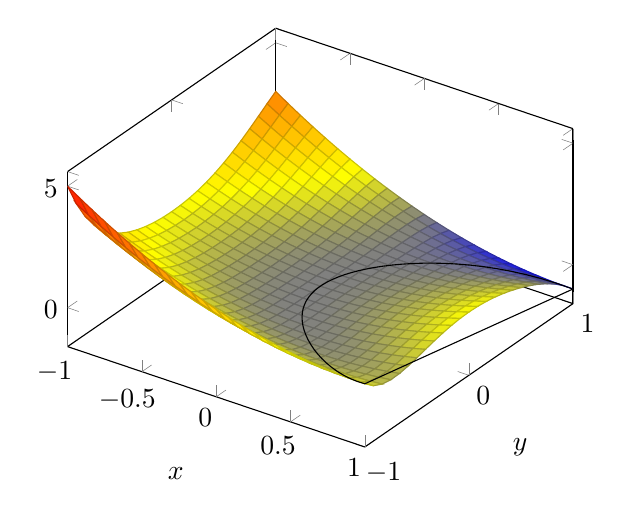
\begin{tikzpicture}
    \begin{axis}[width=8cm,
         3d box=background,
      % pretty printing, but irrelevant:
 %  title={$f(x,y)=x^2-2xy^2+y^4-y^5$},%,\qquad $g(x,y)=x^2+y^2=1$},
   xlabel=$x$, ylabel=$y$,
   view={35}{45}],
   %   xtick=-4:4,
   %   ytick=-4:4,
  ]
  \addplot3[surf,domain=-1:1] {x*x-2*x*y*y+y*y*y*y-y*y*y*y*y};
  \addplot3+[black,domain=-1:1,samples=50,mark=none]
   (x*x,x,-x*x*x*x*x);
 \end{axis}
\end{tikzpicture}
\end{center}
\caption{El campo del ejemplo~\ref{ej:nohessiana} tiene un punto silla en $(0,0)$.}
\label{fig:ej:nohessiana}
\end{figure}
\begin{rawhtml}
<p style="text-align:center">
    <img src="./T2/figuras/Leccion23-fig24.svg"></p>
\end{rawhtml}


\begin{ejemplo}\label{ej:nohessiana}
Vamos a intentar clasificar el punto crítico del campo
\[
f(x,y)=x^2-2xy^2+y^4-y^5
\]
Hallamos el gradiente de $f$ y planteamos el sistema:
\begin{align*}
\nabla f(x,y) & = (2x-2y^2,-4xy+4y^3-5y^4) \\[1em]
\left.\begin{array}{rl}
2x-2y^2 & = 0\\
-4xy+4y^3-5y^4 & =0 
\end{array}\right\} & 
\left.\begin{array}{rl}
x & = y^2\\
-4y^3+4y^3-5y^4 & =0
\end{array}\right\}
\left.\begin{array}{rl}
x & = y^2\\
-5y^4 & =0
\end{array}\right\}
\end{align*}
La única solución de la segunda ecuación es $y=0$ y por lo tanto $(0,0)$ es el único punto crítico.
Para clasificarlo, determinamos la matriz hessiana y la diferencial de segundo orden:
%
\begin{align*}
\nabla^2f(x,y) &=
\begin{pmatrix}
2 & -4y \\
-4y & -4x+12y^2-20y^3
\end{pmatrix}\\
\nabla^2f(0,0) &=
\begin{pmatrix}
2 & 0 \\
0 & 0
\end{pmatrix}\\
d^2f_{(0,0)}(u_1,u_2) &= 2u_1^2
\end{align*}
Por lo tanto, no podemos deducir que $(0,0)$ sea un mínimo, ya que
$d^2f_{(0,0)}(0,1)=0$.

Si consideramos la función $g(t)=f((0,0)+t(0,1))=f(0,t)=t^4-t^5$,
entonces $g^{(4)}(t)=24-120t$ y $g^{(4)}(0)=24>0$;
es decir, 0 es un mínimo de $g(t)$.
Por lo tanto, el estudio de la matriz hessiana y el estudio de la función $g$ nos dice que el
$(0,0)$ es un mínimo local de $f$ restringida a cada recta que pasa por ese punto.
Sin embargo, eso no garantiza que el punto sea mínimo local de $f$. Por ejemplo, consideremos la curva $\gamma(t)=(t^2,t)$; esta curva pasa por el punto $(0,0)$, ya que $\gamma(0)=(0,0)$ en la dirección $(0,1)$, ya que $\gamma'(t)=(2t,1)$ y $\gamma'(0)=(0,1)$.
Si analizamos la función $f$ restringida a esta curva
\[
f(\gamma(t))= f(t^2,t)=t^4-2t^2t^2+t^4-t^5=-t^5
\]
deducimos $f(\gamma(t))\sle 0$ si $t>0$ y $f(\gamma(t))>0$ si $t\sle 0$, por lo que la $(0,0)$ no es extremo local de $f$.
En la figura~\ref{fig:ej:nohessiana} aparece la representación del campo y la curva sobre la que la función toma valores negativos.\fej
\end{ejemplo}

\subsection{Extremos condicionados.
Multiplicadores de Lagrange}

\begin{figure}[t]
\begin{center}
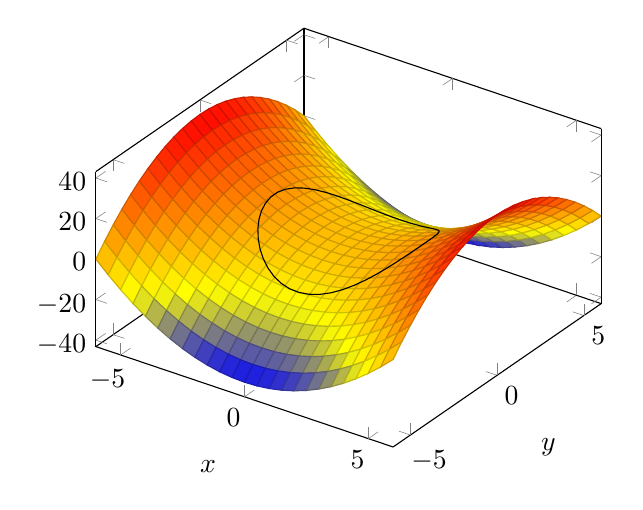
\begin{tikzpicture}
    \begin{axis}[width=8cm,
         3d box=background,
      % pretty printing, but irrelevant:
%   title={$f(x,y)=x^2-y^2$,\qquad $g(x,y)=x^2+y^2=1$},
   xlabel=$x$, ylabel=$y$,
   view={35}{45}],
   %   xtick=-4:4,
   %   ytick=-4:4,
  ]
  \addplot3[surf,domain=-6:6] {x*x-y*y};
  \addplot3+[black,domain=0:360,samples=50,mark=none]
   ({3*cos(x)},
   {3*sin(x)},
   {9*cos(2*x)});
 \end{axis}
\end{tikzpicture}\hfill
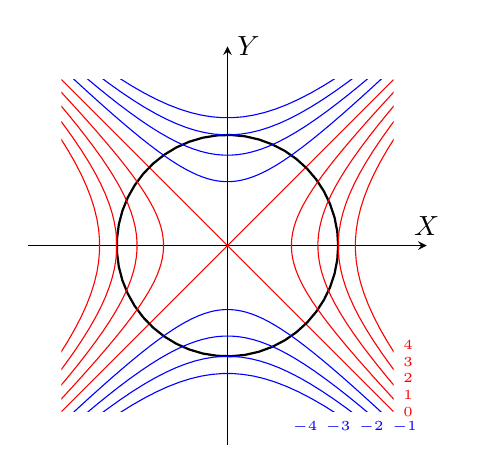
\begin{tikzpicture}[x=4em,y=4em]
\draw[-stealth] (0,-1.8) -- (0,1.8) node[right] {$Y$}; 
\draw[-stealth] (-1.8,0) -- (1.8,0) node[above] {$X$};
%\draw (.15,1.2) node {\scriptsize $1$};
\draw[red] (1.5,-.9) node[right] {\tiny $4$};
\draw[red] (1.5,-1.05) node[right] {\tiny $3$};
\draw[red] (1.5,-1.2) node[right] {\tiny $2$};
\draw[red] (1.5,-1.35) node[right] {\tiny $1$};
\draw[red] (1.5,-1.5) node[right] {\tiny $0$};
%
\draw[blue] (.7,-1.5) node[below] {\tiny $-4$};
\draw[blue] (1,-1.5) node[below] {\tiny $-3$};
\draw[blue] (1.3,-1.5) node[below] {\tiny $-2$};
\draw[blue] (1.6,-1.5) node[below] {\tiny $-1$};
%
\clip (-1.5,-1.5) rectangle (1.5,1.5);
\draw[thin,color=red] (-1.5,1.5)--(1.5,-1.5);
\draw[thin,color=red] (-1.5,-1.5)--(1.5,1.5);
%
\draw[thick,domain=0:360,samples=50,variable=\x]
plot ({cos(\x)},{sin(\x)});
\draw[thin,color=red,domain=-2:2,samples=50,variable=\x]
plot ({.57735*cosh(\x)},{.57735*sinh(\x)});
\draw[thin,color=red,domain=-2:2,samples=50,variable=\x]
plot ({-.57735*cosh(\x)},{.57735*sinh(\x)});
\draw[thin,color=blue,domain=-2:2,samples=50,variable=\x]
plot ({.57735*sinh(\x)},{.57735*cosh(\x)});
\draw[thin,color=blue,domain=-2:2,samples=50,variable=\x]
plot ({.57735*sinh(\x)},{-.57735*cosh(\x)});
%
\draw[thin,color=red,domain=-2:2,samples=50,variable=\x]
plot ({.81649*cosh(\x)},{.81649*sinh(\x)});
\draw[thin,color=red,domain=-2:2,samples=50,variable=\x]
plot ({-.81649*cosh(\x)},{.81649*sinh(\x)});
\draw[thin,color=blue,domain=-2:2,samples=50,variable=\x]
plot ({.81649*sinh(\x)},{.81649*cosh(\x)});
\draw[thin,color=blue,domain=-2:2,samples=50,variable=\x]
plot ({.81649*sinh(\x)},{-.81649*cosh(\x)});
%
\draw[thin,color=red,domain=-2:2,samples=50,variable=\x]
plot ({cosh(\x)},{sinh(\x)});
\draw[thin,color=red,domain=-2:2,samples=50,variable=\x]
plot ({-cosh(\x)},{sinh(\x)});
\draw[thin,color=blue,domain=-2:2,samples=50,variable=\x]
plot ({sinh(\x)},{cosh(\x)});
\draw[thin,color=blue,domain=-2:2,samples=50,variable=\x]
plot ({sinh(\x)},{-cosh(\x)});
%
\draw[thin,color=red,domain=-2:2,samples=50,variable=\x]
plot ({1.1547*cosh(\x)},{1.1547*sinh(\x)});
\draw[thin,color=red,domain=-2:2,samples=50,variable=\x]
plot ({-1.1547*cosh(\x)},{1.1547*sinh(\x)});
\draw[thin,color=blue,domain=-2:2,samples=50,variable=\x]
plot ({1.1547*sinh(\x)},{1.1547*cosh(\x)});
\draw[thin,color=blue,domain=-2:2,samples=50,variable=\x]
plot ({1.1547*sinh(\x)},{-1.1547*cosh(\x)});
%
\end{tikzpicture}
\end{center}
\caption{Representaciones de $f(x,y)=x^2-y^2$ sobre $x^2+y^2=9$.}\label{fig:lagrange1}
\end{figure}
\begin{rawhtml}
<p style="text-align:center">
    <img src="./T2/figuras/Leccion23-fig25.svg"></p>
<p style="text-align:center">
    <img src="./T2/figuras/Leccion23-fig26.svg"></p>
\end{rawhtml}


En la sección anterior hemos afrontado el problema de hallar los extremos locales de un campo
escalar, es decir, los extremos sobre \emph{subconjuntos abiertos} dentro del dominio del campo.
Sin embargo, en muchas ocasiones nos interesará estudiar los extremos sobre conjuntos cuyo interior es vacío;
por ejemplo, estudiar los extremos de un campo sobre $\mathbb{R}^2$ restringiéndonos a una circunferencia.
Esta es la situación que abordamos en esta sección;
concretamente, nos planteamos el siguiente problema:
encontrar los extremos del campo $f(x_1,\dots,x_n)$ sobre un conjunto $S$ definido a partir de $k$ campos escalares $g_i(x_1,\dots,x_n)$,  $1\le k\sle  n$:
\[
S=\{(x_1,\dots,x_n)\in\mathbb{R}^n\mid g_i(x_1,\dots,x_n)=0,\ 1\le i\le k\}
\]
Más brevemente, enunciamos el problema diciendo:
\emph{encontrar los extremos del campo escalar $f$ con las condiciones o restricciones
$g_i(x_1,\dots,x_n)=0$, para cada $i$ tal que $1\leq i\leq k\sle  n$.}

En el ejemplo~\ref{ej:x2-y2} de la página~\pageref{ej:x2-y2} hemos visto que el campo $f(x,y)=x^2-y^2$ no tiene extremos locales, es decir, el campo no alcanza ni máximo ni mínimo sobre ningún conjunto abierto.
Sin embargo, en la figura~\ref{fig:lagrange1}, podemos apreciar que si restringimos el campo a la circunferencia $x^2+y^2=9$, entonces sí aparecen varios extremos.

En el lado derecho de la misma figura~\ref{fig:lagrange1}, vemos la representación del mismo campo, pero mediante las curvas de nivel para $-4$, $-3$, $-2$, $-1$, $0$, $1$, $2$, $3$ y $4$; también representamos la circunferencia $x^2+y^2=9$ sobre la que queremos optimizar el campo.
Si nos fijamos por ejemplo en el punto $(3,0)$ de la circunferencia, observamos que la circunferencia y la curva de nivel que pasa por este punto son tangentes.
Si analizamos los valores del campo según nos desplazamos sobre la circunferencia desde algún punto por debajo de $(3,0)$ hasta algún punto por encima de él, observamos que hasta llegar al $(3,0)$ cortamos curvas de nivel correspondientes a valores crecientes del campo, y a partir de $(3,0)$ cortamos curvas de nivel correspondientes a valores decrecientes del campo.
Por lo tanto, podemos afirmar que $(3,0)$ es un máximo (local) de $f$ sobre la circunferencia.

Este ejemplo, que más adelante completaremos analíticamente, motiva el siguiente resultado que afirma que los candidatos a extremos están entre los puntos tales que el conjunto de la restricción y la curva o superficie de nivel son tangentes.

\begin{teorema} Sean $f,g_1,\dots,g_k\colon \mathit{D}\subset \mathbb{R}^n\to\mathbb{R}$ campos escalares
diferenciables y con derivadas parciales continuas. Sea $S$ el subconjunto de $\mathbb{R}^n$ formado por los puntos que verifican las condiciones
\[
g_i(x_1,\dots,x_n)=0\qquad\text{ para todo } i=1,\dots,k
\]
Si $\boldsymbol{x_0}$ es un extremo
local de $f$ restringida a $S$, y $\{\nabla g_i(\boldsymbol{x_0})\mid 1\le i\le k\}$ es un sistema de vectores no nulos linealmente independientes, entonces existen números reales $\mu_i$ tales que 
\[
\nabla f(\boldsymbol{x_0})=\mu_1\nabla g_1(\boldsymbol{x_0})+\dots +\mu_k\nabla g_k(\boldsymbol{x_0})
\]
A las constantes $\mu_1,\dots,\mu_k$ se las denomina \emph{multiplicadores de Lagrange}
asociados~a~$\boldsymbol{x_0}$.
\end{teorema}
%
La condición
``$\{\nabla g_i(\boldsymbol{x_0})\mid 1\le i\le k\}$ es un sistema de vectores no nulos
linealmente independientes'', exigida en el teorema, se
reduce en la práctica a observar que el problema está bien planteado, es decir, que no hay condiciones superfluas, y que  están dadas \emph{de la mejor forma posible}.
Los ejemplos y ejercicios que planteemos a lo largo del tema estarán formulados de esta forma y, por lo tanto, no será necesario verificar esta condición.

\newpage
Este teorema nos da el primer paso a seguir para la
determinación de los extremos condicionados:
\begin{itemize}
\item
Los extremos locales del campo $f$ con las restricciones 
$g_1=0$,\dots, $g_k=0$, se encuentran entre los puntos $(x_1,\dots ,x_n)$ cuyas
coordenadas son solución del sistema:
\begin{eqnarray*}
&&g_1(x_1,\dots ,x_n)=0\\
&&\qquad \dots\\
&&g_k(x_1,\dots ,x_n)=0\\
&&D_1f(\boldsymbol{x}) = 
\mu_1 D_1g_1(\boldsymbol{x})+\dots +\mu_k D_1g_k(\boldsymbol{x})\\
&&\qquad \dots\\
&&D_nf(\boldsymbol{x}) = 
\mu_1 D_ng_1(\boldsymbol{x})+\dots +\mu_k D_ng_k(\boldsymbol{x})
\end{eqnarray*}
Si $x_1,\dots,x_n,\mu_1,\dots,\mu_k$ es una solución del
sistema, $(x_1,\dots,x_n)$ se denomina \emph{punto crítico} de $f$ con las
restricciones $g_1$,\dots, $g_k$ y
$\mu_1,\dots,\mu_k$ son sus multiplicadores de Lagrange asociados.
\end{itemize}

\begin{figure}
\begin{center}
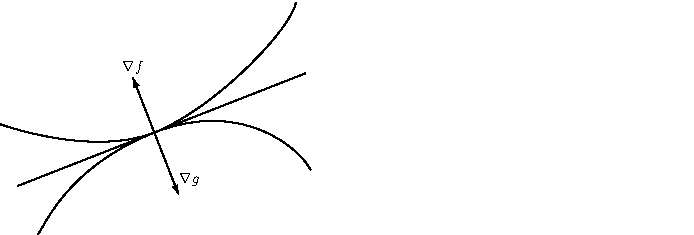
\includegraphics{T2/figs/lagrange.pdf}
\end{center}
\caption{Relación entre gradientes en el método de los multiplicadores de Lagrange.}\label{fig:lag-part}
\end{figure}
\begin{rawhtml}
<p style="text-align:center">
    <img src="./T2/figuras/Leccion23-lagrange.svg"></p>
\end{rawhtml}
%
En particular, si $n=2$ y $k=1$, tanto las curvas de nivel como la restricción son curvas.
Además una curva de nivel es tangente a la restricción en $\boldsymbol x_0$ si los vectores normales en $\boldsymbol x_0$ son iguales o proporcionales, tal y como vemos en la figura~\ref{fig:lag-part}, es decir:
\[
\nabla f(\boldsymbol x_0)= \mu\cdot\nabla g(\boldsymbol x_0)
\]
%
\begin{ejemplo}\label{ej:lag-x2-y2}
Vamos a encontrar los puntos críticos del problema de extremos condicionados de la figura~\ref{fig:lagrange1}:
\begin{alignat*}{2}
f(x,y)=&x^2-y^2\qquad\qquad &g(x,y)&=x^2+y^2-9=0\\
\nabla f(x,y)=&(2x,-2y)& \nabla g(x,y)&=(2x,2y)
\end{alignat*}
El sistema de ecuaciones que tenemos que resolver es:
%
\begin{align*}
0&=x^2+y^2-9\\
2x &= 2x\mu \\
-2y &= 2y\mu
\end{align*}

%
De la segunda ecuación obtenemos que o bien $x=0$ o bien $\mu=1$. En el primer caso obtenemos, por la primera ecuación, las posibilidades $y=3$ o $y=-3$, y por la tercera, $\mu=-1$.
Del caso $\mu=1$, obtenemos de la tercera ecuación que $y=0$, y por la primera llegamos a las posibilidades
$x=3$ o $x=-3$.
De esta forma, los puntos críticos y sus correspondientes multiplicadores son:
\begin{align*}
(3,0) &\to \mu =1\\
(-3,0) &\to  \mu =1\\
(0,-3) &\to  \mu =-1\\
(0,3) &\to  \mu =-1
\end{align*}
%
\begin{figure}[t]
\begin{center}
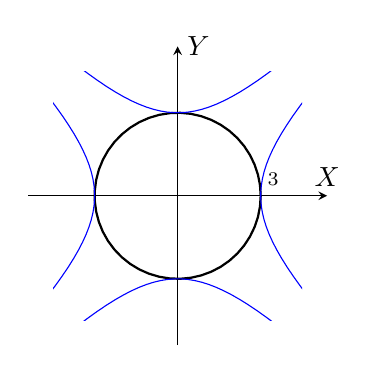
\begin{tikzpicture}[x=3em,y=3em]
\draw[-stealth] (0,-1.8) -- (0,1.8) node[right] {$Y$}; 
\draw[-stealth] (-1.8,0) -- (1.8,0) node[above] {$X$};
\draw (1.15,.2) node {\scriptsize $3$};
%
\clip (-1.5,-1.5) rectangle (1.5,1.5);
\draw[thick,domain=0:360,samples=50,variable=\x]
plot ({cos(\x)},{sin(\x)});
%
\draw[thin,color=blue,domain=-2:2,samples=50,variable=\x]
plot ({cosh(\x)},{sinh(\x)});
\draw[thin,color=blue,domain=-2:2,samples=50,variable=\x]
plot ({-cosh(\x)},{sinh(\x)});
\draw[thin,color=blue,domain=-2:2,samples=50,variable=\x]
plot ({sinh(\x)},{cosh(\x)});
\draw[thin,color=blue,domain=-2:2,samples=50,variable=\x]
plot ({sinh(\x)},{-cosh(\x)});
%
\end{tikzpicture}
\end{center}
\caption{Puntos críticos del ejemplo~\ref{ej:lag-x2-y2}.}
\label{fig:lag-x2-y2}
\end{figure}
\begin{rawhtml}
<p style="text-align:center">
    <img src="./T2/figuras/Leccion23-fig27.svg"></p>
\end{rawhtml}
%
En la figura~\ref{fig:lag-x2-y2} aparecen representadas las dos curvas de nivel tangentes a la restricción, $x^2-y^2=9$, $x^2-y^2=-9$, aunque cada una de ellas tiene dos ramas.\newline
\rule{0pt}{0pt}\hfill\fej
\end{ejemplo}

\begin{rawhtml}
<p style="text-align: center;"><iframe width="560" height="316" src="https://www.youtube.com/embed/duIFDZE9xXw?list=PL2rtpLKW91qYfkQ_gzsN2-UGxdfRYJ03_" frameborder="0" allowfullscreen=""></iframe></p>
\end{rawhtml}


Igual que para los extremos no condicionados, después de calcular los puntos críticos, el problema será decidir cuáles son máximos, cuáles mínimos y cuáles no son extremos. 
Para ello, recurrimos igualmente a la segunda derivada, es decir, a la matriz hessiana tal y como recoge el siguiente resultado.
El teorema establece que, para determinar la naturaleza de un punto crítico $\boldsymbol{a}$, tenemos que estudiar el signo de la forma cuadrática $d^2F_{\boldsymbol a}$ restringiéndonos al subespacio~$T$.


\begin{teorema} Sea $\boldsymbol{a}$ un punto crítico de $f$ sujeto a las restricciones~$g_i=0$,
$1\le i\le k$, y sean $\alpha_1$,\dots, $\alpha_k$ sus multiplicadores de Lagrange. Consideremos el campo $F_{\boldsymbol a}\colon
\mathit{D}\subset\mathbb{R}^n\to\mathbb{R}$ definido por
\[
F_{\boldsymbol a}(\boldsymbol{x})=f(\boldsymbol{x})-\alpha_1g_1(\boldsymbol{x})-\dots -\alpha_kg_k(\boldsymbol{x})
\]
y sea $T$ el espacio vectorial tangente a $S$ en $\boldsymbol{a}$ (la dimensión del subespacio $T$ es $n-k$).
\begin{enumerate}
\item Si $d^2F_{\boldsymbol a}(\boldsymbol{u})>0$ para todo $\boldsymbol{u}\in T$, $\boldsymbol{u}\neq \boldsymbol 0$, entonces $\boldsymbol{a}$ es punto mínimo local.
\item Si $d^2F_{\boldsymbol a}(\boldsymbol{u})\sle 0$ para todo $\boldsymbol{u}\in T$, $\boldsymbol{u}\neq \boldsymbol 0$, entonces $\boldsymbol{a}$ es punto máximo local.
\item Si $d^2F_{\boldsymbol a}(\boldsymbol{u_1})>0$ para algún $\boldsymbol{u_1}\in T$, $\boldsymbol{u}_1\neq \boldsymbol 0$, y  $d^2F_{\boldsymbol a}(\boldsymbol{u_2})\sle 0$ para algún
$\boldsymbol{u_2}\in T$, $\boldsymbol{u}_2\neq \boldsymbol 0$, entonces $\boldsymbol{a}$ no es extremo.
\end{enumerate}
\end{teorema}
%
En cualquier otro caso, no considerado en el teorema anterior, no podemos deducir nada.

Vemos a continuación cómo queda este resultado si lo aplicamos a campos escalares de dos variables y una restricción.
%
\begin{corolario} Sea $(a_1,a_2)$ un punto crítico de $f(x,y)$ sobre~$g(x,y)=0$,
y $\alpha$ su multiplicador de Lagrange;
consideremos el campo\[
F(x,y)=f(x,y)-\alpha g(x,y)
\]
y sea $(u_1,u_2)$ un vector perpendicular a $\nabla g(a_1,a_2)$
\begin{enumerate}
\item Si $d^2F_{(a_1,a_2)}(u_1,u_2)>0$, entonces $(a_1,a_2)$ es punto mínimo local.
\item Si $d^2F_{(a_1,a_2)}(u_1,u_2)\sle 0$, entonces $(a_1,a_2)$ es punto máximo local.
\end{enumerate}
\end{corolario}

Como en el teorema general, si $d^2F_{(a_1,a_2)}(\boldsymbol{u})=0$, {\bf\em no podemos deducir nada}.

Para trabajar con las funciones $F_{\boldsymbol a}$, es conveniente utilizar su definición en términos de $f$ y $g$ y las propiedades de linealidad del vector gradiente y la matriz hessiana:
\begin{align*}
\nabla F_{\boldsymbol a} & = \nabla f -\alpha\nabla g \\
\nabla^2 F_{\boldsymbol a} & = \nabla^2 f -\alpha\nabla^2 g
\end{align*}

\begin{ejemplo}
Anteriormente, hemos calculado los puntos críticos del campo $f(x,y)=x^2-y^2$ sujeto a la restricción 
$g(x,y)=x^2+y^2-9=0$ y hemos visto que estos puntos son 
\begin{align*}
(3,0) &\to \mu =1\\
(-3,0) &\to  \mu =1\\
(0,-3) &\to  \mu =-1\\
(0,3) &\to  \mu =-1
\end{align*}
Vamos a clasificar los puntos críticos $(3,0)$ y $(0,3)$ (los otros dos se clasifican de forma similar).

Para estudiar el punto $(3,0)$ con multiplicador $1$, utilizamos el campo
\begin{align*}
F(x,y)&=f(x,y)-g(x,y)=x^2-y^2-(x^2+y^2-9)=-2y^2+1\\
\nabla F(x,y)&=\nabla f(x,y) -\nabla g(x,y)t=(2x,-2y)-(2x,2y)=
(0, -4y)\\
\nabla^2 F(x,y)&=
\nabla^2 f(x,y) -\nabla^2 g(x,y)=
\begin{pmatrix}
2 & 0\\
0 & -2
\end{pmatrix}-
\begin{pmatrix}
2 & 0\\
0 & 2
\end{pmatrix}=
\begin{pmatrix}
0 & 0\\
0 & -4
\end{pmatrix}\\
\nabla^2 F(3,0)&=
\begin{pmatrix}
0 & 0\\
0 & -4
\end{pmatrix}
\end{align*}
Dado que $\nabla g(x,y)=(2x,2y)$, tenemos que $\nabla g(3,0)=(6,0)$ y un vector perpendicular a él es $\boldsymbol u=(0,1)$.
\[
d^2F_{(3,0)}(0,1)=(0\ 1)
\begin{pmatrix}
0 & 0\\
0 & -4
\end{pmatrix}
\begin{pmatrix}
0\\
1 
\end{pmatrix} = -4 \sle 0
\]
En consecuencia, $(0,3)$ es un máximo local.

Para estudiar el punto $(0,3)$,  con multiplicador $-1$, utilizamos el campo
\begin{align*}
G(x,y)&=f(x,y)+g(x,y)=x^2-y^2+(x^2+y^2-9)=2x^2-9\\
\nabla F(x,y)&=\nabla f(x,y) +\nabla g(x,y)=(2x,-2y)+(2x,2y)=
(4x, 0)\\
\nabla^2 G(x,y)&=
\nabla^2 f(x,y) +\nabla^2 g(x,y)=
\begin{pmatrix}
2 & 0\\
0 & -2
\end{pmatrix}+
\begin{pmatrix}
2 & 0\\
0 & 2
\end{pmatrix}=
\begin{pmatrix}
4 & 0\\
0 & 0
\end{pmatrix}\\
\nabla^2 G(0,3)&=
\begin{pmatrix}
4 & 0\\
0 & 0
\end{pmatrix}
\end{align*}
Dado que $\nabla g(x,y)=(2x,2y)$, tenemos que $\nabla g(0,3)=(0,6)$ y un vector perpendicular a él es $\boldsymbol u=(1,0)$.
\[
d^2G_{(0,3)}(1,0)=(1\ 0)
\begin{pmatrix}
4 & 0\\
0 & 0
\end{pmatrix}
\begin{pmatrix}
1\\
0 
\end{pmatrix} = 4 >0
\]
En consecuencia, $(0,3)$ es un mínimo local.\fej
\end{ejemplo}

\begin{rawhtml}
<p style="text-align: center;"><iframe width="560" height="316" src="https://www.youtube.com/embed/MKcYiVEDM0k?list=PL2rtpLKW91qYfkQ_gzsN2-UGxdfRYJ03_" frameborder="0" allowfullscreen=""></iframe></p>
\end{rawhtml}

Realmente, el método de los multiplicadores de Lagrange solo es estrictamente necesario si no es posible reducir unas variables a otras a partir de las restricciones que determinan el enunciado.
Incluso aunque tal reducción sea posible, el proceso resultante puede ser más complejo;
por ejemplo, en la restricción $x^2+y^2=1$ necesitaríamos cuatro igualdades para hacer esta reducción,
\[
y=\sqrt{1-x^2},\quad
y=-\sqrt{1-x^2},\quad
x=\sqrt{1-y^2},\quad
x=-\sqrt{1-y^2},
\]
y analizar posteriormente todos los puntos obtenidos.
Sin embargo, cuando esta reducción sea asequible y el resultado sea sencillo, será el método más adecuado.
%
\begin{ejemplo}
Vamos a calcular los extremos de $f(x,y,z)=x^2+6y-z^2$, sujeto a las restricciones $2x-y=0$, $y+z=0$, podemos reducir las variables $y$ y $z$,
\begin{align*}
y&=2x\\
z&=-y=-2x
\end{align*}
de forma que el problema es equivalente a obtener los extremos de la función de una variable
\[
g(x)=f(x,2x,-2x)=x^2+6\cdot 2x-(-2x)^2=-3x^2+12x
\]
Para esta función podemos aplicar las técnicas de optimización de funciones de una variable: 
\begin{align*}
g(x) &=-3x^2+12x \\
g'(x) &= -6x+12 \\
g'(x)=0 &\Leftrightarrow x=2\\
g''(x)&=-6\\
g''(2)&=-6\sle 0 \Rightarrow x=2 \text{ es máximo de $g$}
\end{align*}
Por lo tanto, $(2,2\cdot 2,-2\cdot 2)=(2,4,-4)$ es un máximo local del campo~$f$.\fej
\end{ejemplo}

\subsection{Extremos absolutos}\label{sec:absolutos}

Para concluir la lección, vamos a analizar como tendríamos que resolver un problema en el que necesitemos obtener los
extremos absolutos de un campo sobre un conjunto cerrado y acotado $C$.

En primer lugar, dividimos $C$ en dos conjuntos,
$C=U\cup B$, en donde $U$ es el interior de $C$ y $B$ su frontera.
Los candidatos a ser extremos absolutos de $f$ sobre $C$ son:
\begin{enumerate}
\item
Los puntos críticos de $f$ en $U$.% y los puntos de no diferenciabilidad.
\item
Los puntos críticos de $f$ sobre $B$, que pueden ser obtenidos por el método de los multiplicadores de Lagrange, reduciendo variables, considerando distintas secciones en la frontera,\dots
\item
Si hemos dividido la frontera en varias secciones, también deberemos considerar como candidatos los puntos en donde se unen estas secciones.
\end{enumerate}
%
Para determinar los máximos y mínimos absolutos, basta con evaluar $f$ sobre todos los puntos anteriores y determinar cuál es el valor máximo y cuál es el valor mínimo.
%
\begin{figure}
\begin{center}
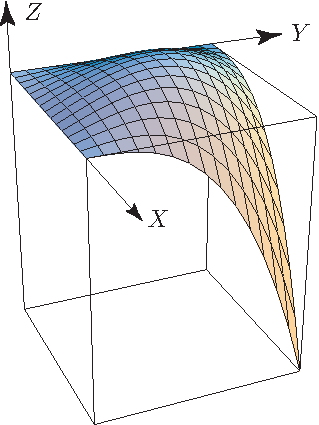
\includegraphics[scale=.6]{T2/figs/max-abs.pdf}
\end{center}
\caption{Representación del ejemplo~\ref{ej:max-abs}.}
\label{fig:max-abs}
\end{figure}
\begin{rawhtml}
<p style="text-align:center">
    <img src="./T2/figuras/Leccion23-max-abs.svg"></p>
\end{rawhtml}
%
\begin{ejemplo}\label{ej:max-abs}
\enlargethispage{.5\baselineskip}
Vamos a determinar los extremos absolutos del campo
\[
f(x,y)=xy(1-x^2-y^2)
\]
en el cuadrado $0\leq x\leq 1$, 
$0\leq y\leq 1$~(ver figura~\ref{fig:max-abs}).

\begin{alignat*}{2}
D_1f(x,y,z)=y-3x^2y-y^3&=0,&\quad
D_2f(x,y,z)=x-3y^2x-x^3&=0\\
y(1-3x^2-y^2)&=0,&\quad
x(1-3y^2-x^2)&=0
\end{alignat*}
Dado que buscamos puntos críticos en el interior del cuadrado, entonces $x\ne 0$, $y\ne 0$.
A partir de las ecuaciones $1-3x^2-y^2=0$ y $1-3y^2-x^2=0$, es fácil deducir que $x=1/2$ e $y=1/2$.
%\begin{align*}
%1-3x^2-y^2 &=0\\
%y^2 & =1-3x^2\\
%1-3y^2-x^2&=0\\
%1-3(1-3x^2)-x^2&=0\\
%1-3(1-3x^2)-x^2&=0\\
%-2+8x^2&=0 \Rightarrow x=1/2
%\end{align*}
%Nuevamente hemos utilizado la restricción del dominio para tomar solo la solución positiva;
%el punto crítico resultante es $(1/2,1/2)$.

Ahora hallamos los puntos críticos en los bordes del cuadrado usando la reducción de variables:
\begin{itemize}
\item
Si $x=0$, $g_1(y)=f(0,y)=0$, y debemos de considerar todos los puntos.
\item
Si $y=0$, $g_2(x)=f(x,0)=0$, y debemos de considerar todos los puntos.
\item
Si $x=1$, $g_3(y)=f(1,y)=-y^3$; el único punto crítico es $y=0$ que queda en el extremo del intervalo.
\item
Si $y=1$, $g_4(x)=f(x,1)=-x^3$; el único punto crítico es $x=0$ que queda en el extremo del intervalo.
\end{itemize}
\enlargethispage{1em}
Ahora solo tenemos que evaluar el campo en todos los puntos obtenidos y en los cuatro vértices del cuadrado para decidir cuál es el máximo y cuál el mínimo.
\begin{align*}
f(1/2,1/2)&= 1/8 \\
f(x,0)&= 0 \\
f(0,y)&= 0 \\
f(1,1)&= -1
\end{align*}
Por lo tanto, $(1/2,1/2)$ es máximo absoluto y $(1,1)$ es mínimo absoluto.%
%\newline
%\ 
\fej
\end{ejemplo}

\begin{rawhtml}
<p style="text-align: center;"><iframe width="560" height="316" src="https://www.youtube.com/embed/bQHF1FYYDQ4?list=PL2rtpLKW91qYfkQ_gzsN2-UGxdfRYJ03_" frameborder="0" allowfullscreen=""></iframe></p>
\end{rawhtml}
	

\subsection{Cálculo de distancias}

Una aplicación de los métodos de optimización es el cálculo de distancias entre lugares geométricos.
Si $A$ y $B$ son dos subconjuntos de~$\mathbb{R}^2$, la distancia entre $A$ y $B$ es la menor de las distancias entre puntos de~$A$ y puntos de~$B$.
Por esta razón, el cálculo de estas distancias suponen la resolución de un problema de optimización en donde la función a optimizar es la distancia entre dos puntos.
  
Recordemos que la distancia ente dos puntos $(a,b)$ y $(c,d)$ es
\begin{equation}\label{ec:distancia}
\sqrt{(a-c)^2+(b-d)^2}
\end{equation}
por lo que esta será la expresión que tendremos que optimizar en los problemas sobre distancias.
Sin embargo, teniendo en cuenta que la función raíz cuadrada es creciente, la expresión~\ref{ec:distancia} será máxima (respectivamente, mínima) si y solo la
siguiente expresión lo es:
\[
(a-c)^2+(b-\mathit d)^2
\]
También podemos usar otras fórmulas ya conocidas para abordar problemas particulares.
Por ejemplo, si uno de los conjuntos es una recta, podemos usar la siguiente fórmula que determina la distancia entre un  punto $(a,b)$ y una recta $Ax+By+C=0$:
\[
\frac{|Aa+Bb+C|}{\sqrt{A^2+B^2}}
\]
También podemos simplificar esta expresión si la usamos en problemas de optimización: para optimizar la distancia de una recta $Ax+By+C=0$, a un lugar geométrico $\mathit D$, consideramos la función
\[
f(x,y)=(Ax+By+C)^2,\qquad (x,y)\in\mathit D
\]

%, podemos razonar como sigue.
%    Si tomamos un punto cualquiera de la recta $(x_0,y_0)$ y tenemos en cuenta que $(A,B)$ es un vector normal a la recta, se verifica que 
%    \[
%    (a-x_0,b-y_0)\cdot (A,B) = \|(a-x_0,b-y_0)\|\|(A,B)\|\cos\alpha
%    \]
%    en donde $\dfrac{\pi}2-\alpha$ es el ángulo que forma la recta con el vector $(a-x_0,b-y_0)$.
%    Pero en este caso, $\|(a-x_0,b-y_0)\|\cos\alpha$ es la proyección del vector $(a-x_0,b-y_0)$ sobre la perpendicular a la recta, es decir, la distancia entre el punto y la recta (ver figura~\ref{fig:dist-recta}).
%    Por lo tanto
%\begin{align*}
%d = & \left|\|(a-x_0,b-y_0)\|\cos\alpha \right|= \\
%    =& \frac{|(a-x_0,b-y_0)\cdot (A,B)|}{\|(A,B)\|}\\
%    =& \frac{|Aa+Bb-Ax_0-By_0|}{\|(A,B)\|} \\
%    =& \frac{|Aa+Bb+c|}{\|(A,B)\|} =\frac{|Aa+Bb+c|}{\sqrt{A^2+B^2}}
%\end{align*}
%
%
%\begin{figure}
%\begin{center}
%\begin{tikzpicture}[x=2.5em,y=2.5em]
%
%%\draw (3,4.5) node[right] {$d$};
%
%\clip (0,1) rectangle (5.5,6.5);
%
%%\draw[step=1] (0,0) grid (10,10);
%\draw (0,0) -- (8,6); 
%\draw[dashed](6.25,0) -- (0,8.33333);
%\draw[color=blue, thick] (2,17/3) -- (4,3);
%\draw[color=blue, thick] (2,1.5) -- (2,17/3) ;
%\draw[fill] (2,17/3) circle (.05);
%\draw (2,1.5) node[left] {$(x_0,y_0)$};
%\draw (2,17/3) node[right] {$(a,b)$};
%\draw (2,3.5) node[left] {$r$};
%\draw (3,4.5) node[right] {$\mathit d$};
%\draw (2,17/3)+(270:1) arc (270:307:1);
%\draw (2.5,4.5) node {$\alpha$};
%%\draw[-stealth] (-1.8,0) -- (1.8,0) node[above] {$X$};
%%\draw (.15,1.2) node {\scriptsize $1$};
%%\draw[red] (1.5,-.9) node[right] {\tiny $4/3$};
%%\draw[red] (1.5,-1.1) node[right] {\tiny $1$};
%%\draw[red] (1.5,-1.3) node[right] {\tiny $1/3$};
%%\draw[red] (1.5,-1.5) node[right] {\tiny $1/3$};
%\end{tikzpicture}\\
%\makebox[22.2em][l]{$\mathit d$ es la distancia de $(a,b)$ a la recta} \\
%\makebox[22.2em][l]{$r=\|(a-x_0,b-y_0)\|$}\\
%\makebox[22.2em][l]{Por lo tanto, $\mathit d = r\cos\alpha = \|(a-x_0,b-y_0)\|\cos\alpha$}
%\end{center}
%\caption{Distancia de un punto a una recta.}\label{fig:dist-recta}
%\end{figure}
%%%    %
%%    Algunos problemas de distancias se pueden resolver más fácilmente utilizando argumentos puramente geométricos.
%%    Por ejemplo, para cálcular la distancia entre un punto $(a,b)$ y una recta $Ax+By+C=0$, podemos razonar como sigue.
%%    Si tomamos un punto cualquiera de la recta $(x_0,y_0)$ y tenemos en cuenta que $(A,B)$ es un vector normal a la recta, se verifica que 
%%    \[
%%    (a-x_0,b-y_0)\cdot (A,B) = \|(a-x_0,b-y_0)\|\|(A,B)\|\cos\alpha
%%    \]
%%    en donde $\dfrac{\pi}2-\alpha$ es el ángulo que forma la recta con el vector $(a-x_0,b-y_0)$.
%%    Pero en este caso, $\|(a-x_0,b-y_0)\|\cos\alpha$ es la proyección del vector $(a-x_0,b-y_0)$ sobre la perpendicular a la recta, es decir, la distancia entre el punto y la recta (ver figura~\ref{fig:dist-recta}).
%%    Por lo tanto
%%    \begin{align*}
%%    \text{Distancia}= & \left|\|(a-x_0,b-y_0)\|\cos\alpha \right|= \\
%%    =& \frac{|(a-x_0,b-y_0)\cdot (A,B)|}{\|(A,B)\|}\\
%%    =& \frac{|Aa+Bb-Ax_0-By_0|}{\|(A,B)\|} \\
%%    =& \frac{|Aa+Bb+c|}{\|(A,B)\|} =\frac{|Aa+Bb+c|}{\sqrt{A^2+B^2}}
%%    \end{align*}
%%    En la penúltima igualdad hemos utilizado que $(x_0,y_0)$ es un punto de la recta, es decir, $Ax_0+By_0+C=0$, o lo que es lo mismo $-Ax_0-By_0=C$.
%%    
%%    Por otra parte, obsérvese que hemos introducido el valor absoluto, ya que la proyección puede ser positiva o negativa según la posición relativa del punto, pero la distancia siempre tiene que ser positiva.
%%


\newpage
\thispagestyle{empty}

\ 

\vfill
\newpage


\section*{Relación de ejercicios \thechapter.1}

\pagestyle{relaciones}

\begin{enumerate}

\item
Represente gráficamente las funciones:
\setcontadoralph
\begin{centrar}
\nitem
$f(x)=x^3+2x^2$\hfill
\nitem
$g(x)=\dfrac{3x^2}{1+x^3}$\hfill
\nitem
$h(x)=\dfrac{x^3}{(2x-1)(2x+1)}$
%$h(x)=\sqrt{x^2+1}-x$
\end{centrar}
\begin{centrar}
\nitem
$\cosh(x)=\dfrac{e^x+e^{-x}}2$\hfill
\nitem
$\operatorname{senh}(x)=\dfrac{e^x-e^{-x}}2$
%$h(x)=\sqrt{x^2+1}-x$
\end{centrar}


\item
Consideramos los puntos $P=(-2,-1)$ y $Q=(3,0)$:
\begin{enumerate}
\item
Defina una parametrización del segmento que va de $P$ a $Q$ usando el intervalo $[0,1]$ como recorrido del parámetro.

\item
Defina una parametrización del segmento que va de $P$ a $Q$ usando el intervalo $[-1,1]$ como recorrido del parámetro.

\item
Defina una parametrización del segmento que va de $Q$ a $P$.

\item
Determine la ecuación general de la recta que pasa por $P$ y $Q$.
\end{enumerate}

\item
Consideramos la curva $C$ definida por la siguiente parametrización:
\[
x(t)=t^2-t\qquad y(t)=t^3-3t\qquad t\in \mathbb{R}.
\]
\begin{enumerate}
\item
Dibuje la curva $C$.

\item
Determine las rectas tangente y normal a $C$ en el punto $(2,2)$,%t=2$
describiéndolas con sus ecuaciones paramétricas y cartesianas.

\item
Determine todos los puntos de tangencia horizontal y vertical de $C$.
\end{enumerate}

\item
Dibuje la curva
\[
x(t)=\dfrac{3t}{1+t^3}\qquad y(t)=\dfrac{3t^2}{1+t^3},\qquad t\in (-\infty,-1)\cup(-1,+\infty)
\]
Determine los puntos de tangencia horizontal y vertical y compruebe que $y=-x-1$ es una asíntota de la curva.


\item
La gráfica de la función $f(\theta)=2\cos\theta+\operatorname{sen} 2\theta$ es la que se muestra abajo.
A partir de esa gráfica, dibuje la curva polar $r=f(\theta)$.
\begin{center}
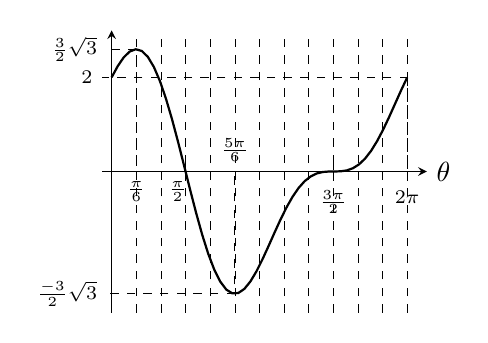
\begin{tikzpicture}[x=1.7em,y=1.7em]
%\draw[thin,dashed,step=.523599] (-.5,-3.3) grid (6.5,3);
\draw[-stealth] (-.2,0) -- (6.7,0) node[right] {$\theta$}; 
\draw[-stealth] (0,-3) -- (0,3);
\draw[thin,dashed] (6.3,2)--(-.2,2) node[left]{\scriptsize$2$};

\draw[very thin,dashed] ( .523599,-3) -- ( .523599,3);
\draw[very thin,dashed] (1.047198,-3) -- (1.047198,3);
\draw[very thin,dashed] (1.570796,-3) -- (1.570796,3);
\draw[very thin,dashed] (2.094395,-3) -- (2.094395,3);
\draw[very thin,dashed] (2.617994,-3) -- (2.617994,3);
\draw[very thin,dashed] (3.141593,-3) -- (3.141593,3);
\draw[very thin,dashed] (3.665191,-3) -- (3.665191,3);
\draw[very thin,dashed] (4.18879,-3) -- (4.18879,3);
\draw[very thin,dashed] (4.712389,-3) -- (4.712389,3);
\draw[very thin,dashed] (5.235988,-3) -- (5.235988,3);
\draw[very thin,dashed] (5.759587,-3) -- (5.759587,3);
\draw[very thin,dashed] (6.283185,-3) -- (6.283185,3);

\draw[thin,dashed] (.5235987755982988,2.4) -- (.5235987755982988,0) node[below]{\scriptsize$\frac{\pi}6$};
\draw[thin,dashed] (1.570796326794897,.2) -- (1.570796326794897,-.2);
\draw (1.4,0) node[below]{\scriptsize$\frac{\pi}2$};
\draw[thin,dashed] (2.617993877991494,-2.4) -- (2.617993877991494,0) node[above]{\scriptsize$\frac{5\pi}6$};
\draw[thin,dashed] (4.71238898038469,.2) -- (4.71238898038469,-.2) node[below]{\scriptsize$\frac{3\pi}2$};
\draw[thin,dashed] (2.617993877991494,-2.598076211353316)--(-.1,-2.598076211353316) node[left]{\scriptsize$\frac{-3}2\sqrt3$};
\draw[thin,dashed] (.5235,2.598076211353316)--(-.1,2.598076211353316) node[left]{\scriptsize$\frac{3}2\sqrt3$};
\draw[thin,dashed] (6.28318,2) -- (6.28318,-.2) node[below]{\scriptsize$2\pi$};
\draw[thick,domain=0:6.28318,samples=50,variable=\x]
plot (\x,{2*cos(\x r)+sin(2*\x r)});
\end{tikzpicture}
\hspace{2em}
\raisebox{-2em}{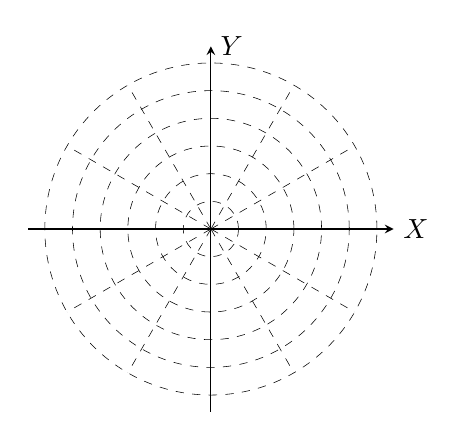
\begin{tikzpicture}[x=2em,y=2em]
\draw[-stealth] (-3.3,0) -- (3.3,0) node[right] {$X$}; 
\draw[-stealth] (0,-3.3) -- (0,3.3) node[right] {$Y$};
\draw[very thin,dashed] (0,0) circle (3);
\draw[very thin,dashed] (0,0) circle (2.5);
\draw[very thin,dashed] (0,0) circle (2);
\draw[very thin,dashed] (0,0) circle (1.5);
\draw[very thin,dashed] (0,0) circle (1);
\draw[very thin,dashed] (0,0) circle (.5);
\draw[very thin,dashed] (0,0)--(30:3);
\draw[very thin,dashed] (0,0)--(60:3);
\draw[very thin,dashed] (0,0)--(120:3);
\draw[very thin,dashed] (0,0)--(150:3);
\draw[very thin,dashed] (0,0)--(210:3);
\draw[very thin,dashed] (0,0)--(240:3);
\draw[very thin,dashed] (0,0)--(300:3);
\draw[very thin,dashed] (0,0)--(330:3);
\end{tikzpicture}}
\end{center}


\item
Dibuje la curva polar $r=2+\operatorname{sen}(4\theta)$, $\theta\in [0,2\pi]$. Halle la ecuación de la recta tangente a esta curva para $\theta=\dfrac\pi2$.

\item
Dibuje la curva polar $r=2-\sec\theta$, $\theta\in (\dfrac{-\pi}2,\dfrac\pi2)$ y compruebe que $x=-1$ es una asíntota de la curva.


\item
Identifique los siguientes lugares geométricos, determine sus características principales, obtenga una parametrización y dibujelas.

\setcontadoralph
\begin{center}
\begin{tabular}{l@{\qquad\quad}l}
\nitem $x^2+y^2-6x+5 = 0$ &
\nitem $x^2+y^2-6x+10 = 0$ \\
\nitem $x^2+y^2-6x+9 = 0$ &
\nitem $x^2-4x-4y^2 =0$ \\
%\nitem $x^2-3x-4y^2 =0$ \\
\nitem $x^2+2x+4y^2-3 =0$ &
\nitem $y^2-4x+2y+5 =0$
%\nitem $y^2-3x+y+1 =0$
\end{tabular}
\end{center}

\item
Determine una parametrización de la elipse con centro en el punto $(1,0)$, ejes paralelos a los ejes de coordenadas y semiejes $\sqrt2$ y $1$.


\item
Probar que el lugar geométrico dado por $\left | z \right |+\left | z+2 \right |= 4 $ con $z \in \mathbb{C}$, es la curva:
\[
3x^{2}+6x+4y^{2}-9=0
\]
siendo $x$ e $y$ la parte real e imaginaria de $z$ respectivamente.
Enumerar sus principales características y dar una parametrización de dicho lugar geométrico.







%EJERCICIOS DE PARAMETRIZAR DE UN CAMINO (VER EJERCICIOS DE INTEGRAL DE LINEA)
%CON PARAMETRIZACIO ́ N EN FUNCIO ́ N DE LA X Y DE LA Y: Funciones y=f(x),
%funciones donde el par ́ametro no sea necesariamente la x, trozos de par ́abola, circunferencia



\end{enumerate}

\newpage
%\thispagestyle{empty}
%
%\ 
%
%\vfill
%\newpage

\section*{Relación de ejercicios \thechapter.2}

\begin{enumerate}


\item
Determine y represente el dominio de los siguientes campos:
\setcontadoralph
\begin{centrar}
\nitem $f(x,y)=\sqrt{1-x^2-y^2}$,\hfill
\nitem $g(x,y)=\log\dfrac{y}{x^2+y^2-1}$.
\end{centrar}

\item
Determine las curvas de nivel de los siguientes campos escalares, representándolas para algunos valores.
\setcontadoralph
\begin{centrar}
\nitem
$f(x,y)=y+\cos 2x$, \hfill
\nitem
$g(x,y)=e^{y-x^2}$,\hfill
\nitem
$h(x,y)=\dfrac{2x^2+y^2}{x-2y}$.
\end{centrar}


\item
Halle el vector gradiente de los siguientes campos.
\setcontadoralph
\begin{centrar}
\nitem $f(x,y) = \log (\operatorname{sen} xy)$\hfill
\nitem $g(x,y,z) = x^2y^3z^4$
\end{centrar}

\item
Calcule la derivada direccional del campo $f(x,y)=x^3+3xy$ en el punto $(1,1)$ a lo largo de la recta
$y=x$ y en la dirección de decrecimiento de $x$.

\item
Encuentre las ecuaciones del plano tangente y de la recta normal al grafo del campo $f(x,y)=\dfrac{x^2}{x+y}$
en el punto $(2,2,1)$.

\item
Encuentre las ecuaciones del plano tangente y la recta normal a la superficie  $x\operatorname{sen} y +x^2e^z=4$ en el punto $(2,\pi ,0)$.

\item
Pruebe que las superficies 
\[
x+y^2+2z^3=4,\qquad\quad 3z\log(y)+13z-12zx=1
\]
son ortogonales en todos los puntos de intersección.
Es decir, las rectas normales a las superficies en estos puntos son ortogonales.

\item
Consideramos la curva
\[
9x^2+4xy+6y^2-14x+8y+10=0
\]
\begin{enumerate}
\item
Halla la recta tangente a la curva en el punto $\big(\frac45,\frac{-3}5\big)$.
\item
Halla los puntos de la curva cuya tangente es horizontal.
\end{enumerate}

\end{enumerate}

\newpage
\thispagestyle{empty}

\ 

\vfill
\newpage

\section*{Relación de ejercicios \thechapter.3}

\begin{enumerate}
\item
Identifique y clasifique (si existen) los puntos
críticos de los siguientes campos:
\setcontadoralph
\begin{center}
\begin{tabular}{ll}
\nitem $f(x,y)=x^3+y^3-3xy$ & 
\nitem $g(x,y)=(x^2+y^2)e^{x-y}$ \\
\nitem
$h(x,y)=2x^4+4x^2+y^2+8xy+4y+3$
\end{tabular}
\end{center}

\item
Determine y clasifique los puntos críticos de $f(x,y)=x^3+y^3$ sobre la restrición $x^2+y^2=1$.

\item
Consideramos el campo \(f(x,y)=3x^2+y^3\):
\begin{enumerate}
\item
Determine, sin clasificar, todos los puntos críticos del campo \(f\) sobre la curva
\(x^2+y^2=9\)
\item
Uno de los puntos obtenidos en el apartado anterior debe ser $(\sqrt{5},2)$: clasifique este punto.
%(0,3), (0,-3), (3,0), (-3,0), (-\sqrt{5},2)
\end{enumerate}



\item
Consideremos la función $f(x,y)=-3xy^2+4y^2-10xy+12y+4x^2-15x+14$. 
\begin{enumerate}
\item
Compruebe que $(1,-1)$ es un punto crítico de $f(x,y)$ sujeto a la condición $x-2y-3\mbox{e}^{x+y}=0$.
\item 
Clasifique el punto crítico del apartado anterior.
\end{enumerate}

\item
Sabemos que $(2,1)$ es un punto crítico de un campo $f(x,y)$ sujeto a la restricción
$x^3+y^2-4xy-y=0$, siendo  $\alpha=\frac12$ el multiplicador de Lagrange y 
$\nabla^2f(2,1)=\begin{pmatrix}5 & 0\\0 & -3\end{pmatrix}$.
Determine si el punto crítico es máximo o mínimo.

\item
Calcule la distancia entre las parábolas $4x^2=8y+7$, $y^2=4x-8$. Indicación: es mejor reducir variables en lugar de usar multiplicadores de Lagrange.
% y posteriormente utilizando simplemente argumentos geométricos.


\item
Aplique el método de los multiplicadores de Lagrange para hallar las distancias máximas y mínimas de un punto de la elipse $x^2+4y^2=5$ a la recta $x+y=4$.
%Indicación: optimice la función que da la distancia entre un punto $(x,y)$ y una recta $AX+BY+C=0$, es decir, $f(x,y)=\dfrac{|Ax+By+C|}{\sqrt{A^2+B^2}}$ con la restricción adecuada.
%obtenida en el primer ejercicio de esta relación.


\item
Halle los valores máximo y mínimo del campo escalar
$f(x,y)=\exp\big(\frac{-xy}4\big)$ en la región $x^2+y^2\leq 2$.


\item 
Halle los valores máximo y mínimo del campo escalar
$f(x,y)=x^2-xy+y^2+1$ en la región triangular cerrada del primer cuadrante acotada por las rectas $x=0$, $y=4$, $y=x$.





\end{enumerate}


\newpage
\thispagestyle{empty}

\ 

\vfill
\newpage

\section*{Relación de ejercicios \thechapter.4}

\begin{enumerate}

\item
Halle la ecuación de la recta tangente a la curva $x=2\cotg(t)$, $y=2\operatorname{sen}^2(t)$, en $t_0=\dfrac{\pi}{4}$

\item
Consideramos la curva: $(x(t),y(t))=\left(\dfrac{2t^2}{1+t^2},\dfrac{2t^3}{1+t^2}\right)$,
$t\in\mathbb{R}$.
\begin{enumerate}
\item
Halle: $\lim_{t\to +\infty}(x(t),y(t))$ y $\lim_{t\to 0}\dfrac{y'(t)}{x'(t)}$.
\item
Dibuje la curva.
%\item
%¿Es una parametrización regular? ¿Es una curva regular?
\end{enumerate}

\item
Halle los puntos de la curva $x=2(t + t\operatorname{sen} t)$,\quad
$y=2(1 -\cos t)$
en los que la tangente sea horizontal.

\item
Halle los puntos de la curva $x=\cos t + t\operatorname{sen} t$,\quad
$y=\operatorname{sen} t - t\cos t$
en los que la tangente sea vertical.

\item
Demuestre que las ecuaciones:
\[
\left\{\begin{array}{l}
x(t)=\dfrac{a(1-t^2)}{1+t^2} \\[.6em]
y(t)=\dfrac{2bt}{1+t^2}
\end{array}\right.
\]
son una parametrización de la elipse $\dfrac{x^2}{a^2}+\dfrac{y^2}{b^2}=1$.
¿Cómo se desplaza un punto por la curva cuando crece el parámetro $t$?


\item
Localice los puntos de tangencia horizontal y vertical, si los hay, de las curvas polares siguientes

\setcontadoralph
\begin{centrar}
\nitem
$r=1+\operatorname{sen}\theta$,\hfill
\nitem
$r=a\operatorname{sen}\theta\cos^2\theta$
\end{centrar}


\item
Dibuje las siguientes curvas dadas en coordenadas polares.
\setcontadoralph
\begin{center}
\begin{tabular}{l@{\qquad}l}
\nitem $r=2+\dfrac{1}{\theta}$ &
\nitem $r=1+\dfrac{1}{2}\cos\theta$ (Caracol de Pascal) \\
\nitem $r=\sqrt{\cos 2\theta}$ &
\nitem $r=4\cos\theta$ (Circunferencia) \\
\nitem $r=\dfrac{16}{5-3\cos\theta}$ (Elipse) &
\nitem $r=\dfrac{2}{1-\cos\theta}$ (Parábola)
\end{tabular}
\end{center}

\item
Determine la ecuación de las asíntotas de la curva $r=2\cos 2\theta\sec\theta$


\item
Halle la ecuación de la recta tangente a la curva $r=\dfrac{6}{2\operatorname{sen}\theta -3\cos\theta}$ en $\theta=\pi$

\newpage
\item Encuentre la ecuación de las circunferencias
descritas a continuación:
\begin{enumerate}
\item Centro $(3,-4)$, radio $\sqrt{30}$
\item Con centro en el segundo cuadrante, tangente a los
ejes de coordenadas y radio $4$.
\item Con centro en $(2,-3)$ y pasando por el punto
$(5,4)$.
\item Que tiene el segmento que une $(-1,2)$ y $(5,-6)$
como diámetro.
\item Que pasa por los puntos $(1,0)$, $(3,4)$ y $(5,0)$.
\end{enumerate}

\item Halle el centro y radio de las siguientes
circunferencias.
\begin{enumerate}
\item $(x-2)^2+(y+3)^2=36$
\item $x^2+y^2-4x+6y=3$
\item $x^2+y^2+8x=9$
\end{enumerate}


\item Dibuje las parábolas $y=x^2-4x-5$\quad e\quad  $y^2-3x+1=0$, determinando el vértice y el eje.
% sus focos, sus vértices y directrices.

\item
Dibuje la elipse $\dfrac{x^2}{9}+\dfrac{y^2}{4}=1$ y determine sus ejes, vértices y focos.

\item
Dibuje la hipérbola $\dfrac{x^2}{16}-\dfrac{y^2}{6}=1$
y determine su ejes, focos, vértices y asíntotas.


\item
Describe el lugar geométrico determinado por:
\begin{enumerate}
\item %(Elipse)
$\left | z-1 \right |+\left | z+3 \right |= 10$       \item %(Circunferencia)
$\left | z-2i \right |= 1$
\item %(circulo de centro (0,2) y radio 1)
$\left | z-2i \right |\leqslant 1 $       
\end{enumerate}





\item
Determine el dominio de los siguientes campos:
\setcontadoralph
\begin{center}
\begin{tabular}{l@{\qquad}l}
\nitem $f(x,y)=\dfrac{1}{y}\cos x^2$ &
\nitem $f(x,y)=\dfrac{x^2-y^2}{x-y}$\\
\nitem $f(x,y)=\log (1-xy)$ &
\nitem $f(x,y)=\log (x^2+y^2)$ \\
\nitem $f(x,y)=\dfrac{x}{\sqrt{x^2+y^2}}$ &
\nitem $f(x,y)=\dfrac{\operatorname{sen} (x^2+y^2)}{x^2+y^2}$ 
\end{tabular}
\end{center}

\item
Describa las curvas de nivel de los siguientes campos y dibuje algunas. Esboce sus gráficas:
\setcontadoralph
\begin{center}
\begin{tabular}{l@{\qquad}l}
\nitem $f(x,y)=2x+y$ &
\nitem $f(x,y)=\cos(2x+y)$ \\
\nitem $f(x,y)=y^2-x$ &
\nitem $f(x,y)=\sqrt{x^2+y^2-1}$
% \\
%\nitem $f(x,y)=\arctg(y-x)$
\end{tabular}
\end{center}


\item
Halle el vector gradiente de los siguientes campos:
\setcontadoralph
\begin{centrar}
\nitem $f(x,y)=e^x\cos y$,\hfill
%\nitem $f(x,y,z) = x^{y^z}$,\hfill
\nitem $f(x,y) = \operatorname{tg} (x^2+y^2)$
\end{centrar}

\item
Calcule la derivada direccional del campo $f(x,y)=x^2+y\operatorname{senh} (xy)$ en el punto $(2,0)$, a lo largo de la recta tangente a la curva $y=\sqrt{x+7}-3$ en la dirección de decrecimiento de $x$.

\item
Encuentre la ecuación del plano o recta tangente 
a la superficie o curva en el punto indicado, así como
la de la recta normal: 
\begin{center}
\setcontadoralph
\begin{tabular}{l@{\quad}l}
\nitem $x\operatorname{sen} y +x^2e^z=4$ en $(2,\pi ,0)$, &
\nitem $x^3y-\dfrac{x^2}{y}=4$ en $(2,1)$ \\
\nitem $xz^2+\dfrac{(2x-z)^2}{y^3}=19$ en $(2,1,3)$,& 
\nitem $3xe^y+xy^3=2+x$ en $(1,0)$ \\
\nitem $z=\operatorname{sen} xy$ en $(1,\pi /2,1)$, &
\nitem $z=\dfrac{x^2}{x+y}$ en $(2,2,1)$\\
\nitem $z=\log (x^2+y)$ en $(1,0,0)$, &
\nitem $z=x^2e^{xy}$ en $(3,0,9)$
\end{tabular}
\end{center}

\item
Encuentre el punto de la superficie $z=xy$ en donde la
recta normal es paralela a la recta $x=3-2t$, $y=4+5t$,
$z=3+3t$.

\item
Encuentre el punto de la superficie $z=x^2+y^2$
en donde el plano tangente es paralelo al
plano $6x-4y+2z=5$.

\item
Encuentre todos los puntos de la superficie
$z=x^2y$ en donde el plano tangente es ortogonal a la recta $x=2-6t$, $y=3-12t$, $z=2+3t$.

\item
Pruebe que las siguientes superficies 
son ortogonales en todos los puntos de intersección:
\[
x^2-2y^2+z^2=0,\qquad xyz=1,
\]

\item
Consideramos la siguiente superficie: $\quad
\displaystyle x\,\mbox{e}^{x+y}+y\,\mbox{e}^{A(y+z)}+z\,\mbox{e}^{B(z-x)} = 1$

Determine los valores de $A$ y $B$ para que el plano tangente a la superficie en el punto $(1,-1,1)$ sea paralelo al plano $-2x+2y+z=3$ y proporcione dicho plano tangente.



\item
Identifique y clasifique los puntos
críticos de las siguientes funciones:
\begin{center}
\setcontadoralph
\begin{tabular}{l@{\qquad}l}
\nitem $z=x^2-2xy+y^3$ &
\nitem $z=x^2y-2xy$ \\
\nitem $z=2x^2-xy-3y^2-3x+7y$ &
\nitem $z=x^2-xy+y^2-2x+y$ \\
\nitem $z=(5x+7y-25)e^{-(x^2+xy+y^2)}$ &
\nitem $z=x\,\mbox{e}^x-(1+\mbox{e}^x)\cos y$ \\ %(0,2k\pi), (-2,(2k+1)\pi) Mins - sillas
\end{tabular}
\end{center}

\item
Determine y clasifique los puntos críticos de 
$z=e^{2x+3y}(8x^2-6xy+3y^2)$.

\item
Determine y clasifique los puntos críticos de $f(x,y)=y\,x^2\,\mbox{e}^{xy}$.
% Sin hessiana, hay que usar regiones

\item
Determine y clasifique los puntos críticos de
$f(x,y,z)=x^2+y^2+7z^2-xy$

\item
Determine y clasifique los puntos críticos de
$f(x,y)=x^2x+y^2z+\frac23z^3-4x-4y-10z+1$.
%(2,2,1)PS, (-2,-2,-1)PS (1,1,2)min (-1,-1,-2)max 


\item
Encuentre el máximo y el mínimo absoluto del campo
\[
f(x,y)=\frac{-1}{\sqrt{x^2+y^2}}
\]
en el conjunto de puntos tales que $(x-5)^2+y^2\le1$.

\item
Determine y clasifique los puntos críticos del campo escalar
$$ 
f(x,y)=4y-2x-x^2y
$$ 
sujeto a la condición $xy=-1$.


\item
En los siguientes apartados, halle los máximos y mínimos
absolutos de las funciones en los dominios dados:
\begin{enumerate}
\item
$f(x,y)=x^2+xy+y^2-6x$ en la placa rectangular $0\leq x \leq 5$,
$-3\leq y \leq 3$.
\item
$g(x,y)=48xy-32x^3-24y^2$ en la placa rectangular $0\leq x \leq 1$,
$0\leq y \leq 1$.
\end{enumerate}

\item
Halle los valores máximo y mínimo del campo $f(x,y)=x^2y(4-x-y)$ en el triángulo limitado por las rectas $x=0$, $y=0$, $x+y=6$.

\item 
Consideremos el campo escalar:
\[
f(x,y)=-xy^2+11y^2+4xy+10y+x^2+x+5
\]

\begin{enumerate}
\item
Comprueba que $(2,-1)$ es un punto crítico de $f$.
\item
Halla $\nabla^2f(2,-1)$ y $d^2f_{(2,-1)}(u,v)$.
\item
Clasifica el punto crítico $(2,-1)$.
\end{enumerate}

\item
Consideremos la función $f(x,y)=3x^2+3y^2-10xy+4x+4y$.
Demuestre que $(-1,-1)$ es un punto crítico de $f$ sobre la restricción $x^2+y^2=2$ y clasifíquelo.

\end{enumerate}

%% Las lineas siguientes se añaden si la última página está en blanco
% \newpage
%
%\ \thispagestyle{empty}

%\newpage
%\thispagestyle{empty}
%
%\ 
%
%\vfill
%\begin{center}
%(Esta página se ha dejado intencionalmente en blanco)
%\end{center}

\endinput
